\documentclass{article}

\PassOptionsToPackage{authoryear,round}{natbib}
\usepackage{paper_style}

\usepackage[utf8]{inputenc}
\usepackage[T1]{fontenc}
\usepackage{amsmath,amssymb,amsthm,mathtools}
\usepackage{amsfonts}
\usepackage{bbm}
\usepackage{algorithm}
\usepackage[noend]{algpseudocode}
\usepackage{booktabs}
\usepackage{enumitem}
\usepackage{xcolor}
\usepackage[colorlinks=true,linkcolor=blue,citecolor=blue,urlcolor=blue,hyperfootnotes=false]{hyperref}
\usepackage[nameinlink,noabbrev]{cleveref}
\makeatletter
\renewcommand{\theHALG@line}{\thealgorithm.\arabic{ALG@line}}
\makeatother

\theoremstyle{plain}
\newtheorem{theorem}{Theorem}
\newtheorem{lemma}{Lemma}
\newtheorem{proposition}{Proposition}
\newtheorem{corollary}{Corollary}

\theoremstyle{definition}
\newtheorem{remark}{Remark}
\newtheorem{assumption}{Assumption}

\crefname{assumption}{Assumption}{Assumptions}
\Crefname{assumption}{Assumption}{Assumptions}
\crefname{lemma}{Lemma}{Lemmas}
\Crefname{lemma}{Lemma}{Lemmas}

\newcommand{\E}{\mathbb{E}}
\newcommand{\Var}{\mathrm{Var}}
\newcommand{\Prob}{\mathbb{P}}
\newcommand{\R}{\mathbb{R}}
\newcommand{\1}{\mathbbm{1}}
\newcommand{\Pzero}{P_0}
\newcommand{\psihat}{\widehat{\psi}_{\mathrm{cal}}}
\newcommand{\mhat}{m}
\newcommand{\fhat}{f_n}
\newcommand{\what}{\widehat w}
\newcommand{\wzero}{w_0}
\newcommand{\rhozero}{\rho_0}
\newcommand{\rhon}{\rho_n}
\newcommand{\mtilde}{m_n^\star}
\newcommand{\muzero}{\mu_0}
\newcommand{\Pl}{\mathbb{P}^{L}_n}
\newcommand{\Pu}{\mathbb{P}^{U}_N}
\newcommand{\Px}{P_{0,X}}
\newcommand{\M}{\mathcal M}
\newcommand{\Cov}{\operatorname{Cov}}


\usepackage{fvextra}

\DefineVerbatimEnvironment{codeblock}{Verbatim}{
  breaklines=true,
  breakanywhere=true,
  fontsize=\small
}

\title{Calibeating Prediction-Powered Inference}

\author{
Lars van der Laan\\
Department of Statistics, University of Washington\\[0.75em]
Mark van der Laan\thanks{Targeted ML Solutions, \href{https://www.targetedml.com/}{targetedml.com}}\\
Department of Statistics and Division of Biostatistics,\\
Center for Targeted Machine Learning and Causal Inference,\\
University of California, Berkeley
}
\date{\today}

\begin{document}
\maketitle
 
\begin{abstract}
We study semisupervised mean estimation with a small labeled sample, a large unlabeled sample, and a black-box prediction model whose output may be miscalibrated. A standard approach in this setting is augmented inverse-probability weighting (AIPW) \citep{robins1994estimation}, which protects against prediction-model misspecification but may be inefficient when the prediction score is poorly aligned with the outcome scale. We introduce \emph{Calibrated Prediction-Powered Inference}, which post-hoc calibrates the prediction score on the labeled sample before using it for semisupervised estimation. This simple step requires no retraining and can \emph{calibeat} the original score, improving it both as a predictor of the outcome and as a regression adjustment for semisupervised inference. We study both linear and isotonic calibration. For isotonic calibration, we establish first-order optimality guarantees: isotonic post-processing can improve predictive accuracy and estimator efficiency relative to the original score and simpler post-processing rules, while no further post-processing of the fitted isotonic score yields additional first-order gains. For linear calibration, we show first-order equivalence to PPI++. We also clarify the relationship between existing estimators, showing that the original PPI estimator is a special case of AIPW and can be inefficient when the prediction model is accurate, while PPI++ is AIPW with empirical efficiency maximization \citep{rubin2008empirical}. In simulations and real-data experiments, our calibrated estimators often outperform PPI and are competitive with, or outperform, AIPW and PPI++. We provide an accompanying \texttt{Python} package, \href{https://larsvanderlaan.github.io/ppi-aipw/}{\texttt{ppi\_aipw}}.
\end{abstract}
 
 
\section{Introduction}

We study semisupervised mean estimation with one labeled dataset \(\{(X_i, Y_i)\}_{i=1}^n\) and one unlabeled dataset \(\{\widetilde X_i\}_{i=1}^N\), where outcomes are observed only for a subset sampled completely at random. This is a classical missing-outcome problem: rich covariate information is available for many individuals, but the outcome of interest is observed only for a smaller subset. Such settings arise when gold-standard outcomes are expensive to collect but prediction scores are readily available, for example in randomized trials with prognostic models trained on historical data \citep{schuler2022increasing}, biobank analyses using phenotype predictors built from EHR or omics measurements \citep{hong2019semisupervised,zhang2019phecap}, and computational biology pipelines that supplement slow or costly experimental measurements with model-based predictions \citep{ppi2023,crossppi2024}.

The goal is to use the larger unlabeled sample to improve estimation of a population mean while accounting for prediction error. This problem has long been studied in missing-data and semiparametric statistics, where methods such as AIPW, TMLE, and related debiased estimators combine flexible machine-learning prediction with valid inference \citep{robins1994estimation,vanderlaanunified,van2006targeted,vanderLaanRose2011,DoubleML}. More recently, closely related ideas have reappeared in the machine-learning literature under the name prediction-powered inference \citep{ppi2023,angelopoulos2023ppi,crossppi2024}. Similar questions also arise in covariate adjustment for randomized trials, where machine-learning predictors trained on auxiliary data can improve precision in small samples \citep{hansen2008prognostic,rubin2008empirical,moore2009covariate,lin2013agnostic,benkeser2021improving,schuler2022increasing,demirel2024prediction,jin2026prognostic}.


 

A standard approach is to use the labeled sample to debias a plug-in estimator based on a prediction model. If \(m(X)\) is a black-box prediction score, the plug-in estimator averages \(m(X)\) over the pooled covariate sample, while the labeled sample is used to estimate the residual correction term \(\E\{Y-m(X)\}\). For example, the augmented inverse-probability weighted (AIPW) estimator \citep{robins1994estimation} averages \(m(X)\) over both labeled and unlabeled samples and then adds the average residual over the labeled sample, whereas the standard PPI estimator \citep{ppi2023} averages \(m(X)\) only over the unlabeled covariates before applying the same residual correction. The latter is generally less efficient because it discards information in the labeled covariates.

These estimators protect against bias from an imperfect prediction model, but they typically treat \(m(X)\) as fixed. This can be problematic because efficiency depends on how well \(m(X)\) serves as a regression adjustment, that is, on how well it approximates the conditional mean of \(Y\), not merely on whether it ranks observations correctly. A score may be informative for ranking individuals while still being poorly calibrated, in the sense that its numerical values systematically overstate or understate the outcome. In that case, the residuals \(Y-m(X)\) remain unnecessarily variable, and the resulting semisupervised estimator can be far from efficient. Such miscalibration may arise because the model was trained on a different population, or because of temporal drift, distribution shift, or regularization bias.

This motivates post-hoc calibration. Rather than correcting only the marginal bias \(\E\{Y-m(X)\}\), one can use the labeled sample to transform \(m(X)\) so that its numerical values better align with the outcomes they are meant to predict \citep{zadrozny2001obtaining,zadrozny2002transforming,niculescu2005predicting}. An ideal target is a \textit{perfectly calibrated} score \(m_n^\star(X)\) satisfying
\[
\E\!\left[Y \mid m_n^\star(X)\right] = m_n^\star(X).
\]
Post-hoc calibration can improve the regression adjustment, and thus efficiency, without retraining the underlying model. Classical post-processing methods include Platt scaling \citep{platt1999probabilistic}, linear calibration \citep{mincer1969evaluation}, histogram binning \citep{zadrozny2001obtaining}, and isotonic regression \citep{zadrozny2002transforming}. Such methods are especially relevant for modern machine-learning predictors, such as neural networks, which are often informative yet systematically miscalibrated \citep{bella2010calibration,guo2017calibration,wang2023calibration}. Figure~\ref{fig:toy-calibration-ppi} illustrates this mechanism in a simple example: post-hoc calibrating a mis-scaled prediction score improves both predictive accuracy and the efficiency of prediction-powered mean estimation.
 



\paragraph{Contributions.}
We make three main contributions.

First, in Section~\ref{sec:calppi}, we introduce \emph{calibrated prediction-powered inference} for semisupervised mean estimation with a small labeled sample and a larger unlabeled one. The basic idea is to use the labeled data to post-hoc calibrate an existing prediction score before using it for semisupervised estimation. This framework accommodates familiar calibration methods, including linear calibration, Platt scaling, histogram binning, and isotonic regression; see, in particular, Sections~\ref{sec:linear} and \ref{sec:iso}. We focus especially on linearly calibrated PPI and isotonic-calibrated PPI, which are simple to implement, require no tuning, and can be added to an existing prediction pipeline without retraining the original model.

Second, we show that calibration addresses an important limitation of standard AIPW and PPI estimators: a prediction score may rank observations well while still be poorly aligned with the outcome scale, thereby leaving efficiency gains unrealized. In our setting, post-hoc calibration can improve the score as a regression adjustment, yielding sharper point estimates and confidence intervals, while still leading to a simple plug-in estimator. It can also make the fitted score first-order optimal against further post-processing within a specified class, both for prediction and for semisupervised estimation. In the spirit of \citet{foster2023calibeating}, we refer to these two properties as \emph{prediction calibeating} and \emph{functional-estimation calibeating}, respectively.

 

Third, we develop asymptotic theory for linearly calibrated and isotonic-calibrated PPI estimators. For linear calibration, we show that PPI++ is asymptotically equivalent to linearly calibrated PPI, a form of prognostic-score regression adjustment. For isotonic calibration, Section~\ref{sec:theory} establishes asymptotic normality, valid inference, and efficiency guarantees. In particular, isotonic-calibrated PPI achieves the smallest asymptotic variance among estimators based on monotone transformations of the original score, and is therefore at least as efficient as AIPW and PPI based on the uncalibrated score. We also show that the fitted isotonic score cannot be improved by further post-processing for prediction, and that the resulting mean estimator is first-order equivalent to the oracle estimator based on the conditional mean of the outcome given the calibrated score.

Our calibrated PPI framework can be viewed as a semisupervised specialization of the calibrated debiased machine learning framework developed by \citet{van2024automatic}. Our estimators can also be interpreted as targeted minimum loss estimators \citep{van2006targeted,vanderLaanRose2011}, with calibration playing the role of the targeting step.

Section~\ref{sec:setup} reviews the two-sample semisupervised model, the AIPW, PPI, and PPI++ estimators, and the main efficiency concepts used throughout the paper. Section~\ref{sec:exp} presents synthetic and real-data experiments.

\textbf{Code.} The accompanying \texttt{Python} package, reproduction code, and documentation are publicly available at
\href{https://github.com/Larsvanderlaan/ppi-aipw}{github.com/Larsvanderlaan/ppi-aipw}. An interactive package website with examples and API documentation is available at
\href{https://larsvanderlaan.github.io/ppi-aipw/}{larsvanderlaan.github.io/ppi-aipw/}. Self-contained code is provided in Appendix~\ref{appendix:code}.



 \begin{figure*}[h]
\centering
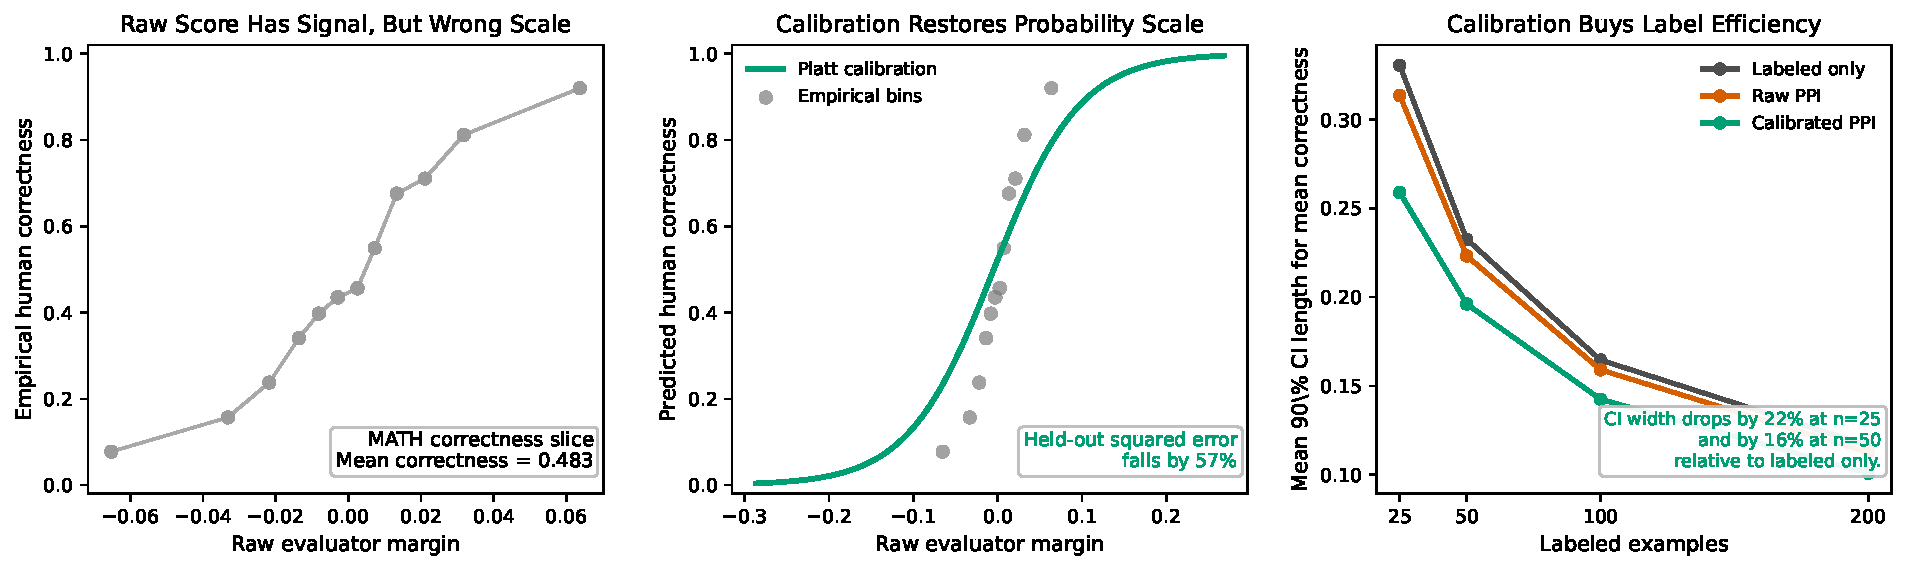
\includegraphics[width=\textwidth]{assets/fig_toy_calibration_ppi.pdf}
\caption{Toy example illustrating how calibration can improve prediction-powered mean estimation. The example is derived from the MATH slice of a public LLM-evaluation benchmark with binary human correctness labels, using the ArmoRM evaluator's raw margin as the prediction score. The target is the average human correctness \(\psi=\mathbb{E}[Y]\), estimated from a small labeled sample together with many unlabeled evaluator scores. Left: the raw margin contains clear signal about correctness, but it is not on the correct numerical scale. Middle: a one-dimensional Platt calibration fit on 100 labeled examples maps the raw margin to estimated correctness probabilities and reduces held-out squared error by about \(57\%\). Right: in Monte Carlo experiments with \(N=2000\) unlabeled scores, calibrated PPI yields substantially shorter \(90\%\) confidence intervals for \(\psi\) than both labeled-only estimation and raw PPI; the mean interval length is about \(17\%\) smaller at \(n=25\) labeled examples and about \(15\%\) smaller at \(n=50\).}
\label{fig:toy-calibration-ppi}
\end{figure*}




\subsection{Related work}
Although PPI has been presented as a recent development, the underlying statistical problem and several closely related estimators lie within a much broader literature on semiparametric debiasing and regression adjustment, including work on missing data, causal inference, and debiased machine learning. In particular, the use of machine-learning predictions to improve efficiency under missing at random outcomes is closely connected to the literature on covariate adjustment in randomized trials and causal inference \citep{moore2009covariate,benkeser2021improving,hojbjerre2025powering}, while power-tuning ideas can be viewed as a form of empirical efficiency maximization \citep{rubin2008empirical}.

 

\textbf{Semiparametric statistics and missing data.} This paper builds on foundational ideas from the missing-data and semiparametric literatures. \citet{rubin1976} formalized missing at random as a key identification condition for recovering full-data targets from partially observed outcomes. Semiparametric efficiency theory then characterized efficient influence functions, regular asymptotically linear estimators, and one-step debiased procedures \citep{levit1975efficiency,pfanzagl1985contributions,hasminskii1979nonparametric,klaassen1987consistent,bickel1993efficient}. In missing-data and causal-inference problems, these ideas led to influence-function-based estimating equations \citep{robins1994estimation,robins1995analysis,robins1995semiparametric,vanderlaanunified,tsiatis2006semiparametric}, often with doubly robust structure \citep{bang2005doubly}. As a result, the efficiency theory for missing-data models under missingness or coarsening at random is now well understood, and the class of regular asymptotically linear estimators in these models can be characterized through their influence functions \citep{robins1994estimation,robins1995analysis,robins1995semiparametric,vanderlaanunified,tsiatis2006semiparametric}.

\textbf{Debiased machine learning and targeted learning.}
A large body of work combines the semiparametric framework above with machine-learning-based nuisance estimation, often under the label of debiased machine learning. Flexible learning methods within estimating equations and AIPW-style procedures appear in early work such as \citet{vanderlaanunified}. Targeted minimum loss estimation (TMLE), or targeted learning, updates an initial nuisance estimator in a parameter-targeted way to produce a plug-in estimator with reduced first-order bias; in the present setting, the primary nuisance estimated by machine learning is the outcome regression \citep{van2006targeted,vanderLaanRose2011,gruber2009targeted,hoffman2020tmle,ross2025constructing}. These approaches are often combined with sample splitting and cross-fitting to accommodate generic machine-learning estimators \citep{schick1986asymptotically,klaassen1987consistent,zheng2010asymptotic,vanderLaanRose2011,DoubleML}. Double machine learning emphasizes similar ingredients---orthogonality, cross-fitting, and influence-function expansions---for inference with modern nuisance estimators \citep{DoubleML,chernozhukov2022automatic}, and is a closely related semiparametric framework \citep{vanderlaan2019cvtmle,diaz2020machine,chen2026equivalence}. For sufficiently stable estimators, cross-fitting can itself be relaxed \citep{chen2022stable}. Closely related work studies balancing-weight estimators \citep{hainmueller2012entropy,imai2014covariate,zubizarreta2015stable,lendle2015balancing,chattopadhyay2020balancing,hejazi2023revisiting}, which often admit equivalent regression-adjustment or augmented representations \citep{chattopadhyay2023implied,bruns2025augmented,rotnitzky2025note}. In missing-at-random settings with known missingness probability, including semisupervised learning and randomized trials, doubly robust estimators typically permit valid inference under flexible nuisance estimation even when the learned regression adjustment is misspecified \citep{moore2009covariate,moore2009increasing,rosenblum2009using,hojbjerre2025powering,hojbjerre2026within}.
  
 
\textbf{Semisupervised inference and improving power in randomized trials.}
Related work studies semisupervised or surrogate-assisted estimation in settings where the primary outcome is observed only on a limited subset, while auxiliary outcomes or surrogate measurements are available more broadly \citep{pepe1992inference,pepe1994auxiliary,chen2000miscellanea,chen2008improving,cheng2021robust,ji2025predictions,kallus2025role}. Two-sample semisupervised inference is a special case of two-stage sampling designs \citep{scott1982effect,rose2011targeted,hejazi2021efficient,qiu2026efficient} and, more generally, of data fusion, for which a substantial semiparametric efficiency literature has been developed \citep{li2023efficient,li2025data,graham2024towards,xu2025unified}. More recent papers have used the term \emph{prediction-powered inference} (PPI) for the semisupervised mean-estimation setting in which a black-box predictor is combined with a small labeled sample and a large unlabeled sample \citep{ppi2023,angelopoulos2023ppi,crossppi2024,xu2025unified,song2026demystifying,poulet2025prediction,wang2025efficient,lee2026mec}. These papers also brought such methods to a broader machine-learning audience and provided accessible software. Closely related questions have long been studied in randomized trials, where prognostic scores or other regression adjustments learned from larger historical, external-control, or auxiliary data sources are used to improve precision in smaller trials \citep{hansen2008prognostic,rosenblum2009using,moore2009covariate,moore2009increasing,moore2011robust,vanderweele2019selecting,benkeser2021improving,burger2021use,schuler2022increasing,li2023estimating,balzer2024adaptive,van2024covariate,hojbjerre2025powering,yang2026improving}. Methodologically, however, PPI estimators can often be viewed as instances or refinements of existing semiparametric procedures. For example, PPI++ is an AIPW estimator \citep{robins1994estimation,vanderlaanunified} obtained by empirical efficiency maximization \citep{rubin2008empirical} over a scaling parameter, while cross-PPI \citep{crossppi2024} is a cross-fitted AIPW estimator \citep{zheng2010asymptotic,DoubleML}. More fundamentally, in settings with known missingness probability, the ability to combine black-box prediction models with valid semiparametric inference is closely tied to the robustness properties of AIPW and is therefore not unique to semisupervised mean estimation \citep{bang2005doubly,seaman2018introduction,rotnitzky2021characterization}.
 

\textbf{Calibrated DML and Recalibrated PPI.}
In our mean-estimation setting, the closest precursor is the calibrated debiased machine-learning framework of \citet{van2024automatic}, which studies calibration of the outcome regression in AIPW estimators for doubly robust inference. Our setting can be viewed as a semisupervised specialization of that perspective, adapted to prediction-powered inference and aimed at improving efficiency in randomized designs. This connection also motivates our term \emph{calibrated PPI}. A related paper is \citet{ji2025predictions}, who study recalibrated prediction-powered inference for general estimating equations. Rather than correcting the predictive model itself, their approach modifies the imputed loss in the PPI estimating equation, thereby ``recalibrating” the estimator rather than the predictions. In the mean-estimation setting under squared loss, the target correction reduces to the conditional mean of the outcome given the initial prediction score, which is also the efficient regression adjustment in the reduced model based only on that score. Thus, this conditional mean may be viewed as an oracle calibrator. The main differences lie in the estimators, emphasis, and theory. \citet{ji2025predictions} use flexible machine learning to estimate this oracle target and thereby pursue semiparametric efficiency \citep{robins1994estimation}. They do not study specific calibration procedures, and their method remains in AIPW form. By contrast, we study simple, widely used post-hoc calibration maps applied directly to a fixed score, and ask what can be guaranteed even without consistent estimation of the oracle target. Our estimators retain a simple plug-in form, yielding lightweight methods that can be incorporated into an existing prediction pipeline without retraining. We also develop calibration-specific results: an exact AIPW interpretation of the plug-in estimator, first-order equivalence between linear calibration and PPI++, and a first-order calibeating guarantee for isotonic calibration.
 


\textbf{From missing data to causal inference.} From the perspective of estimation and efficiency theory, semisupervised mean estimation with missing-at-random outcomes is equivalent to randomized experiments, controlled trials, and survey-sampling designs once the missingness indicator is reinterpreted as a treatment or sampling indicator, so that the relevant potential outcomes are viewed as missing \citep{rubin1978bayesian,vanderlaanunified,licausal,mozer2026ppi}. This equivalence allows tools from covariate adjustment, causal inference, and model-assisted estimation to be transferred directly to the semisupervised setting; see, for example, \citet{mozer2026ppi} for results relating prediction-powered inference to model-assisted survey-sampling estimators. The two-sample formulation we study is also equivalent to a one-sample i.i.d.\ model \citep{li2023efficient}. In particular, our methods apply to inference on the counterfactual mean \(\mathbb{E}[Y(1)]\) in a randomized trial with binary treatment, where treated units form the labeled sample and control units contribute covariate information only; see Appendix~\ref{app:causal}.

 
 
 
\textbf{Calibration.} A final relevant thread concerns calibration. Classical post-processing methods such as Platt scaling \citep{platt1999probabilistic,cox1958two,gupta2023online}, linear calibration \citep{mincer1969evaluation,chernozhukov2018generic,leng2021calibration}, isotonic regression \citep{zadrozny2002transforming,niculescu2005predicting}, and histogram binning \citep{zadrozny2001obtaining,gupta2021distribution} improve predictive reliability without retraining the underlying model. The idea has deeper roots in the forecasting literature \citep{mincer1969evaluation,lichtenstein1977calibration,vovk1992universal,vovk2005algorithmic,gneiting2007probabilistic,lambert2011elicitation}; see also the historical discussion in \citet{lee2023t}. More recent work studies calibration under broader losses and prediction tasks \citep{jung2021moment,noarov2023statistical,van2023causal,whitehouse2024orthogonal,van2025venn}, as well as applications to conformal prediction \citep{van2024self,van2025venn}, importance-weight stabilization \citep{gutman2022propensity,deshpande2023calibrated,ballinari2024improving,van2024stabilized}, treatment effect estimation \citep{chernozhukov2018generic,van2023causal,whitehouse2024orthogonal}, and value prediction in offline reinforcement learning \citep{van2025bellman,van2025semiparametric}. Distribution-free guarantees for histogram binning are developed by \citet{gupta2021distribution}, while \citet{van2023causal,van2025venn} establish asymptotic distribution-free guarantees for isotonic calibration.
 
 \section{Two-Sample Semisupervised Setup}
\label{sec:setup}

\subsection{Data structure and notation}

We observe two independent datasets,
\[
\mathcal D_L=\{(X_i,Y_i)\}_{i=1}^n
\qquad\text{and}\qquad
\mathcal D_U=\{\widetilde X_j\}_{j=1}^N.
\]
The labeled sample consists of i.i.d.\ draws from a distribution \(P_0\) on \(\mathcal X\times\mathbb R\), while the unlabeled sample consists of i.i.d.\ draws from the distribution \(\Px\) of \(X\) under \(P_0\). Our target is the population mean
\[
\psi_0 := \E_{P_0}[Y],
\qquad
\muzero(x):=\E_{P_0}[Y\mid X=x].
\]
This can also be written as
\[
\psi_0=\int y\,dP_0(x,y)=\int \muzero(x)\,d\Px(x).
\]

For functions \(a:\mathcal X\times\mathbb R\to\mathbb R\) and \(b:\mathcal X\to\mathbb R\), define the empirical means over the labeled and unlabeled samples by
\[
\Pl a := \frac{1}{n}\sum_{i=1}^n a(X_i,Y_i),
\qquad
\Pu b := \frac{1}{N}\sum_{j=1}^N b(\widetilde X_j).
\]
For readability, we will sometimes write \(\Pl\{a(X,Y)\}\) instead of \(\Pl a\). When a function depends only on \(X\), we also write
\[
\Pl\{b(X)\}:=\frac{1}{n}\sum_{i=1}^n b(X_i).
\]
We write expectations and variances as \(\E_{P_0}[\cdot]\), \(\E_{\Px}[\cdot]\), \(\Var_{P_0}[\cdot]\), and \(\Var_{\Px}[\cdot]\). 

Throughout, let \(M:=n+N\) and \(\rho_n:=n/M\) denote the labeled fraction. Then
\[
\frac{1}{n+N}\left\{\sum_{i=1}^n f(X_i)+\sum_{j=1}^N f(\widetilde X_j)\right\}
=
\rho_n \Pl\{f(X)\} + (1-\rho_n)\Pu\{f(\widetilde X)\}.
\]
In other words, the empirical mean of \(f(X)\) over the pooled covariate sample is a weighted average of the empirical means from the labeled and unlabeled samples.

\begin{assumption}[Two-sample design]
\label{assump:design}
The following hold:
\begin{enumerate}[leftmargin=6mm,label=(\roman*)]
\item \(\mathcal D_L\) is i.i.d.\ from \(P_0\), and \(\mathcal D_U\) is i.i.d.\ from \(\Px\).
\item \(\mathcal D_L\) and \(\mathcal D_U\) are independent.
\item \(Y\) has finite second moment under \(P_0\).
\item With \(M:=n+N\), the labeled fraction \(\rhon=n/M\) satisfies \(\rhon\to\rhozero\) for some \(\rhozero\in(0,1)\).
\end{enumerate}
\end{assumption}

\begin{remark}
The labeled sample carries the outcome information, while the unlabeled sample sharpens estimation of the marginal covariate distribution. The pooled i.i.d.\ missing-data formulation in Appendix~\ref{app:iid} is a special case of this two-sample setup.
\end{remark}

\subsection{Review of AIPW, PPI, and semiparametric efficiency}
\label{sec:effreview}

\textbf{The AIPW class.}
We begin with the augmented inverse-probability weighted (AIPW) estimator in the unrestricted two-sample model \citep{robins1994estimation}. A useful perspective is that AIPW is not a single estimator, but a family indexed by a score function \(f:\mathcal X\to\R\) with finite second moment. For any such \(f\), define
\begin{equation}
\label{eq:aipw-family}
\widehat\psi(f)
:=
\rhon \Pl\{f(X)\}
+
(1-\rhon)\Pu\{f(\widetilde X)\}
+
\Pl\{Y-f(X)\}.
\end{equation}
This estimator combines a plug-in term based on \(f(X)\) with a residual correction from the labeled sample. For any fixed \(f\), \(\widehat\psi(f)\) is unbiased in finite samples for \(\psi_0=\E_{P_0}[Y]\). In particular, taking \(f(X)=0\) yields the empirical mean estimator \(\Pl\{Y\}\). Thus, within the AIPW class, the choice of \(f\) affects efficiency but not validity: even a poor score does not induce bias, but it can leave substantial precision gains unrealized. In this sense, AIPW is a ``safe'' estimator \citep{xu2025unified}. This property can be viewed as a particularly simple instance of double robustness\footnote{In more general missing-at-random settings with unknown, covariate-dependent missingness probabilities, the analogous AIPW estimator remains doubly robust asymptotically, but it no longer enjoys the same finite-sample unbiasedness as in the present known-\(\rho_n\) setting \citep{seaman2018introduction}.} \citep{bang2005doubly}.

This viewpoint is important for our purposes. Since validity is guaranteed for any \(f\), the central question is how to choose or improve the score to make \(\widehat\psi(f)\) as efficient as possible. In particular, efficiency depends on how well \(f(X)\) approximates the conditional mean of \(Y\), not merely on whether it ranks observations correctly. The same principle underlies the use of flexible machine learning for covariate adjustment in randomized trials while retaining valid inference \citep{moore2009covariate,moore2009increasing,schuler2022increasing,hojbjerre2025powering}.


\textbf{Asymptotic linearity, efficiency, and the role of residual variance.} To characterize the leading large-sample error in the two-sample model, we decompose the estimation error into one contribution from the labeled sample and one from the unlabeled sample. We say that \(\widehat\psi\) is asymptotically linear with influence pair \((D^L,D^U)\) if
\[
\widehat\psi-\psi_0
=
\frac{1}{M}\sum_{i=1}^n D^L(X_i,Y_i)
+
\frac{1}{M}\sum_{j=1}^N D^U(\widetilde X_j)
+
o_p(M^{-1/2}),
\]
where \(\E_{P_0}[D^L(X,Y)]=0\) and \(\E_{\Px}[D^U(\widetilde X)]=0\). By the central limit theorem and the independence of the two samples,
\[
\sqrt{M}\,(\widehat\psi-\psi_0)
\rightsquigarrow
N\!\left(0,\,
\rhozero \Var_{P_0}[D^L(X,Y)]
+
(1-\rhozero)\Var_{\Px}[D^U(\widetilde X)]\right).
\]
The influence pair therefore determines the estimator's asymptotic variance and provides a convenient way to compare efficiency across different choices of \(f\). The next result uses this representation to characterize the AIPW class, identify the efficient influence pair in the unrestricted two-sample model, and thereby obtain the semiparametric efficiency bound \citep{bickel1993efficient}.

\begin{proposition}[Influence pair for the AIPW class]
\label{prop:aipw-class}
Under \cref{assump:design}, for any fixed \(f:\mathcal X\to\R\) with finite second moment, the estimator \(\widehat\psi(f)\) is asymptotically linear with influence pair \((D_f^L,D_f^U)\), where
\begin{align*}
D_f^L(X,Y)
&=
\tilde f(X)-\psi_0+\rhozero^{-1}\{Y-\tilde f(X)\},\\
D_f^U(\widetilde X)
&=
\tilde f(\widetilde X)-\psi_0,
\end{align*}
with \(\tilde f(X):=f(X)-\E_{\Px}[f(X)]+\psi_0\)
denoting the recentered version of \(f(X)\). The resulting asymptotic variance of \(\sqrt{M}\,(\widehat\psi(f)-\psi_0)\) is
\begin{align*}
\Var[\mu_0(X)]
+
\rhozero^{-1}\E_{P_0}\!\bigl[\Var[Y\mid X]\bigr]
+
\frac{1-\rhozero}{\rhozero}\Var_{P_0}[f(X)-\mu_0(X)].
\end{align*}
This variance is minimized over the AIPW class when \(\tilde f=\mu_0\), in particular at \(f=\mu_0\). Therefore, the efficient influence pair for \(\psi_0=\E_{P_0}[Y]\) in the unrestricted two-sample model is \((D_{\mu_0}^L,D_{\mu_0}^U)\), and the corresponding asymptotic variance is the efficiency bound\footnote{Appendix~\ref{section::plugin} shows that every regular estimator is asymptotically equivalent to \(\widehat\psi(f)\) for some score function \(f\). Thus, the AIPW family characterizes the full class of regular estimators and the semiparametric efficiency bound in this model.}.
\end{proposition}

A key implication of Proposition~\ref{prop:aipw-class} is that the asymptotic variance of the AIPW estimator based on \(f\) exceeds the efficiency bound by
\[
\frac{1-\rho_0}{\rho_0}\Var_{P_0}[f(X)-\mu_0(X)].
\]
Thus, within the AIPW class, efficiency is governed entirely by how well \(f(X)\) approximates the conditional mean \(\mu_0(X)\), up to an additive constant; a related observation was made in \cite{wang2025efficient}. In particular, ranking alone is not enough: a score may order observations correctly and still be inefficient if its numerical values are poorly aligned with the outcome scale. Full efficiency therefore generally requires access to the full covariate information \(X\), or at least to a summary rich enough to recover \(\mu_0(X)\) \citep{robins1994estimation,robins1995semiparametric}. This motivates using a flexible black-box prediction score \(m(X)\) for regression adjustment in practice, and motivates post-hoc calibration when that score is informative but misaligned with the conditional mean.

 
Two particularly popular choices in \eqref{eq:aipw-family} are AIPW and PPI. The most common choice is \(f(X)=m(X)\), where \(m(X)\) is a prediction score, yielding the usual augmented inverse-probability weighted (AIPW) estimator \citep{robins1994estimation}:
\[
\widehat{\psi}_{\mathrm{AIPW}}
=
\frac{1}{M}\left\{
\sum_{i=1}^n m(X_i)
+
\sum_{j=1}^N m(\widetilde X_j)
+
\frac{1}{\rho_n}\sum_{i=1}^n \{Y_i-m(X_i)\}
\right\},
\]
where \(\rho_n^{-1}\) is the inverse probability of observing the outcome.

Another estimator in this class was considered by \citet{ppi2023} under the name PPI,\footnote{The PPI and PPI++ estimators are algebraically equivalent to the model-assisted survey-design estimators of \citet{cassel1976some} and \citet{sarndal2003model}, respectively; see \citet{mozer2026ppi} for a review.} defined by
\[
\widehat{\psi}_{\mathrm{PPI}}
=
\Pu\{m(\widetilde X)\}+\Pl\{Y-m(X)\},
\]
which implicitly corresponds to the choice \(f(X)=m(X)/(1-\rho_n)\). Relative to \(\widehat{\psi}_{\mathrm{AIPW}}\), \(\widehat{\psi}_{\mathrm{PPI}}\) places the plug-in term entirely on the unlabeled sample and rescales the score by the factor \((1-\rho_n)^{-1}>1\). By Proposition~\ref{prop:aipw-class}, this improves efficiency only when the rescaled score is closer to \(\mu_0(X)\) in mean squared error. Consequently, PPI is inefficient when \(m=\mu_0\) and is typically less efficient when \(m\) is already reasonably accurate \citep{han2012note,rotnitzky2012improved}. For this reason, we view AIPW as the more natural default in practice.

\textbf{Improving over a class of AIPW estimators through empirical efficiency maximization.}  Because both \(\widehat{\psi}_{\mathrm{AIPW}}\) and \(\widehat{\psi}_{\mathrm{PPI}}\) use scores in the scaling class \(\{\lambda m(X):\lambda\in\mathbb R\}\), it is natural to choose the scaling factor data-adaptively rather than fixing it in advance. One way to do so is to minimize the estimator's empirical influence-function variance over this class:
\[
\sigma_n^2(f)
:=
\rho_n \Pl\left[\left\{f(X)-\widehat{\psi}(f)+\rho_n^{-1}(Y-f(X))\right\}^2\right]
+
(1-\rho_n)\Pu\left[\left\{f(\widetilde X)-\widehat{\psi}(f)\right\}^2\right].
\]
That is, one chooses \(\lambda\) to minimize \(\sigma_n^2(f)\) over \(f(X)=\lambda m(X)\), a procedure known as empirical efficiency maximization \citep{rubin2008empirical,vanderlaanunified}. The resulting estimator, called PPI++ by \citet{angelopoulos2023ppi}, is simply an AIPW estimator with an empirically rescaled prediction rule \(\hat\lambda m(X)\), where \(\hat\lambda\) estimates the population-optimal scaling coefficient
\begin{equation}
\label{opt:scale}
\lambda^\star
=
\frac{\Cov\bigl(Y,m(X)\bigr)}{\Var\bigl(m(X)\bigr)}.
\end{equation}
The same principle extends beyond simple rescaling. For example, one can minimize \(\sigma_n^2(f)\) over richer classes such as
\[
\{\lambda m(X)+\beta_{\mathrm{lin}}^\top X:
\lambda \in \mathbb R,\ \beta_{\mathrm{lin}} \in \mathbb R^d\},
\]
over monotone transformations of the score, or over a reproducing kernel Hilbert space; see Appendix~\ref{appendix:remarks}. More generally, the same criterion can be used in cross-validation to choose among candidate estimator classes \citep{rubin2008empirical}. In particular, if many prediction models \(\{m_1(X),m_2(X),\dots\}\) are available, one could learn a weighted linear combination by minimizing the empirical variance.
 
 
\section{Calibrated Prediction-Powered Inference}
\label{sec:calppi}

Standard AIPW and prediction-powered estimators treat the prediction score \(m(X)\) as fixed. In many applications, however, an available score may be useful for ranking individuals while still being poorly calibrated, in the sense that its numerical values do not accurately reflect the outcome itself. For example, a score may correctly assign higher values to individuals with larger outcomes on average, yet still systematically understate or overstate the conditional mean. Since the efficiency of a semisupervised estimator depends on the quality of the regression adjustment, such miscalibration can leave substantial efficiency gains unrealized.

Motivated by this observation, we study a simple post-hoc strategy: calibrate \(m(X)\) using the labeled sample, then plug the calibrated score into the semisupervised mean estimator. We call the resulting approach \emph{calibrated prediction-powered inference}. As we show below, this yields a simple plug-in estimator with an exact AIPW representation. Different choices of calibration class yield different calibrated PPI estimators, including the linear and isotonic procedures studied below.

\subsection{General estimator and exact AIPW representation}

Let \(m:\mathcal X\to\mathbb R\) be a black-box regression model fit using external data or a separate training sample. We post-process this score on the labeled sample by learning a map \(f_n:\mathbb R\to\mathbb R\), and define the calibrated score
\[
\mtilde := f_n \circ m.
\]
Our estimator averages the calibrated predictions over the pooled labeled and unlabeled samples:
\begin{equation}
\label{eq:plugin}
\psihat
:=
\frac{1}{n+N}\left\{\sum_{i=1}^n \mtilde(X_i) + \sum_{j=1}^N \mtilde(\widetilde X_j)\right\}.
\end{equation}
Equivalently,
\[
\psihat
=
\rhon \Pl\{\mtilde(X)\} + (1-\rhon)\Pu\{\mtilde(\widetilde X)\}.
\]

At a high level, calibration seeks to transform the original score \(m(X)\) into a new score \(\mtilde(X)\) that is better aligned with the outcome. Ideally,
\[
\mtilde(X)\approx \E_{P_0}[Y\mid \mtilde(X)],
\]
so that among individuals with the same predicted value, the average outcome is close to that value. Under squared error loss, calibration is also closely tied to optimal post-processing, since replacing \(\mtilde(X)\) by \(\E_{P_0}[Y\mid \mtilde(X)]\) cannot increase mean squared error. In our setting, this matters because a better regression adjustment yields a more efficient semisupervised estimator. A natural population benchmark is therefore $\E_{P_0}[Y\mid m(X)],$
the best predictor obtainable from the original score alone. Our goal is to move \(m(X)\) toward this benchmark through post-processing, without retraining the underlying model and without requiring that it be estimated accurately.

We learn the post-processing map by empirical risk minimization over a class \(\mathcal H\) of functions \(h:\mathbb R\to\mathbb R\):
\begin{equation}
\label{eq:H-erm}
f_n \in \arg\min_{h\in\mathcal H} \Pl\bigl[(Y-h(m(X)))^2\bigr].
\end{equation}
Assume that \(\mathcal H\) contains the constant functions. Then the corresponding first-order condition implies
\[
\Pl\!\left\{Y-\mtilde(X)\right\}=0.
\]
Therefore, \(\psihat\) is exactly the AIPW estimator \(\widehat{\psi}(\mtilde)\) based on the post-processed score \(\mtilde(X)\):
\begin{align}
\label{eqn::aipwcal}
\psihat
=
\rhon \Pl\{\mtilde(X)\}
+ (1-\rhon)\Pu\{\mtilde(\widetilde X)\}
+ \Pl\{Y-\mtilde(X)\}.
\end{align}
Important examples we will consider later include linear and isotonic calibration, corresponding to \(\mathcal H\) equal to the classes of affine and monotone functions, respectively.

So far, we have described calibration informally as a population property: the score should be interpretable as a prediction of the outcome and should admit no further improvement within a prescribed transformation class. Since the true distribution \(P_0\) is unknown, we instead impose an empirical analogue on the labeled sample. Let \(\mathcal F\) be a linear class of maps \(f:\mathbb R\to\mathbb R\) containing the constants. We say that \(\mtilde\) is \textit{empirically calibrated} over \(\mathcal F\) if
\begin{equation}
\label{eq:cal-risk}
\Pl\bigl[(Y-\mtilde(X))^2\bigr]
\le
\Pl\bigl[(Y-f(\mtilde(X)))^2\bigr],
\qquad
\text{for all } f\in\mathcal F.
\end{equation}
Because \(\mathcal F\) is linear, this is equivalent to the orthogonality condition
\begin{equation}
\label{eq:cal-score}
\Pl\bigl[f(\mtilde(X))\{Y-\mtilde(X)\}\bigr]=0,
\qquad
\text{for all } f\in\mathcal F.
\end{equation}
As we show next, empirical calibration yields not only the exact AIPW representation in \eqref{eqn::aipwcal}, but also a first-order equivalence to an oracle AIPW estimator based on the best population transformation of the fitted score within \(\mathcal F\).

\begin{theorem}[Representation relative to the population-optimal transformation]
\label{thm:repr}
Let \(m_n^\star\) satisfy \eqref{eq:cal-score} over a linear class \(\mathcal F\) containing the constant functions. Define
\[
m_{0,\mathcal F}^\dagger := f_{0,\mathcal F}\circ m_n^\star, \qquad
f_{0,\mathcal F}\in \arg\min_{f\in\mathcal F}
\E_{P_0}\!\left[(Y-f(m_n^\star(X)))^2\right].
\]
Then
\begin{align*}
\psihat
&=
\rhon \Pl\{m_{0,\mathcal F}^\dagger(X)\}
+ (1-\rhon)\Pu\{m_{0,\mathcal F}^\dagger(\widetilde X)\}
+ \Pl\{Y-m_{0,\mathcal F}^\dagger(X)\} \\
&\qquad
+ (1-\rhon)(\Pu-\Pl)\{m_n^\star-m_{0,\mathcal F}^\dagger\}.
\end{align*}
\end{theorem}

Theorem~\ref{thm:repr} is the key structural result. It shows that \(\psihat\) differs from the AIPW estimator based on \(m_{0,\mathcal F}^\dagger\), the population-optimal transformation of \(m_n^\star\) within \(\mathcal F\), only through the remainder
\[
(1-\rhon)(\Pu-\Pl)\{m_n^\star-m_{0,\mathcal F}^\dagger\}.
\]
If \(m_n^\star\) is close to \(m_{0,\mathcal F}^\dagger\) in mean squared error, this term is higher order, so \(\psihat\) and the oracle AIPW estimator have the same first-order asymptotic behavior. In this sense, empirical calibration makes the fitted score behave as though it had already been optimally transformed within \(\mathcal F\). It also yields a balancing-weights representation of the form \(\Pl\{\hat w_{\mathrm{bal}}(X)Y\}\); see Appendix~\ref{app:repr}. We make this precise for isotonic calibration in Section~\ref{sec:theory}.


\textbf{Why calibration can improve efficiency.}
Calibration can improve efficiency by improving the regression adjustment in the exact AIPW representation \eqref{eqn::aipwcal}. If \(f_n\) converges to a population minimizer \(g_0\in\mathcal H\), then the post-processed score \(\mtilde=f_n\circ m\) typically converges to
\[
m_0(X):=g_0\{m(X)\},
\qquad
g_0\in\arg\min_{g\in\mathcal H}
\E_{P_0}\!\left[\{Y-g(m(X))\}^2\right].
\]
Thus, \(m_0\) is the best regression adjustment obtainable from the original score \(m\) using transformations in \(\mathcal H\). By Proposition~\ref{prop:aipw-class}, when \(\mathcal H\) contains the constant functions, minimizing prediction error over the class \(\{\theta\circ m:\theta\in\mathcal H\}\) is first-order equivalent to maximizing AIPW efficiency over the same class. Consequently, the resulting AIPW estimator has asymptotic variance no larger than that of any estimator based on \(\theta\circ m\) with \(\theta\in\mathcal H\). In particular, if the identity map belongs to \(\mathcal H\), then calibration cannot do worse than using the raw score \(m\). If \(\mathcal H\) contains the oracle map \(t\mapsto \E_{P_0}[Y\mid m(X)=t]\), then \(m_0(X)=\E_{P_0}[Y\mid m(X)]\), and the resulting estimator is semiparametrically efficient in the reduced model based on the score \(m(X)\) \citep{ji2025predictions}.

\textbf{Full versus linear calibration.}
We focus on two main cases. In \emph{full calibration}, the target class \(\mathcal F\) is unrestricted, so that at the population level no further transformation of the calibrated score can reduce mean squared prediction error. In practice, however, the fitted map \(f_n\) is learned over a restricted optimization class \(\mathcal H\), which serves as a regularizer. Important examples include piecewise-constant and monotone classes, corresponding to histogram and isotonic calibration; see Section~\ref{sec:iso}. In \emph{linear calibration}, both \(\mathcal H\) and \(\mathcal F\) are restricted to affine maps \(t\mapsto a+bt\), corresponding to least-squares fitting of the working model \(a+b\,m(X)\); see Section~\ref{sec:linear}.
 
 
\subsection{Isotonic-calibrated PPI}
\label{sec:iso}

We focus on isotonic regression as a simple nonparametric post-hoc calibration method \citep{zadrozny2001obtaining,zadrozny2002transforming,niculescu2005predicting}. Let \(\mathcal F_{\mathrm{iso}}\) denote the class of nondecreasing real-valued functions. We fit the calibrator using the labeled pairs \(\{(\mhat(X_i),Y_i)\}_{i=1}^n\) by solving
\[
\hat f \in \arg\min_{f \in \mathcal F_{\mathrm{iso}}}
\sum_{i=1}^n \bigl\{Y_i - f(\mhat(X_i))\bigr\}^2,
\]
and define the calibrated score
\[
m_{n,\mathrm{iso}}^\star(X) = \hat f\{\mhat(X)\}.
\]
The resulting isotonic-calibrated PPI estimator is
\[
\widehat{\psi}_{\mathrm{iso}}
:=
\frac{1}{n+N}
\left\{
\sum_{i=1}^n m_{n,\mathrm{iso}}^\star(X_i)
+
\sum_{j=1}^N m_{n,\mathrm{iso}}^\star(\widetilde X_j)
\right\}.
\]
Isotonic-calibrated PPI is particularly attractive because it is lightweight, tuning-free, and easy to implement with widely available software. Its population target is the monotone transformation of the prediction score \(m(X)\) that minimizes mean squared error, and therefore performs at least as well as the original score and any other monotone transformation of \(m(X)\), including positive rescalings. Thus it yields the best regression adjustment available within the class of monotone transformations of \(m(X)\).


Isotonic regression fits naturally into the \((\mathcal H,\mathcal F)\) framework with \(\mathcal H=\mathcal F=\mathcal F_{\mathrm{iso}}\), the class of nondecreasing functions. Moreover, because the fitted isotonic score is piecewise constant on the blocks learned by the pooled-adjacent-violators algorithm (PAVA) \citep{barlow1972isotonic}, any further transformation of the fitted score is constant on those same blocks. In turn, isotonic calibration yields full empirical calibration.

\begin{proposition}[Isotonic calibration is fully calibrated]
\label{prop:iso-repr}
For every function \(h:\R\to\R\),
\begin{equation}
\label{eq:orth}
\Pl\bigl[h(m_{n,\mathrm{iso}}^\star(X))\{Y-m_{n,\mathrm{iso}}^\star(X)\}\bigr]=0.
\end{equation}
Moreover, for any \(\theta \in \mathcal{F}_{\mathrm{iso}}\),
\[
\Pl\bigl[(Y-m_{n,\mathrm{iso}}^\star(X))^2\bigr]
\le
\Pl\bigl[(Y-\theta(\mhat(X)))^2\bigr].
\]
In particular,
\[
\Pl\bigl[(Y-m_{n,\mathrm{iso}}^\star(X))^2\bigr]
\le
\Pl\bigl[(Y-\mhat(X))^2\bigr].
\]
\end{proposition}


 

  

 

\begin{algorithm}[t]
\caption{Isotonic-calibrated PPI}
\label{alg:isoppi}
\begin{algorithmic}[1]
\Require \(\mathcal D_L=\{(X_i,Y_i)\}_{i=1}^n\), \(\mathcal D_U=\{\widetilde X_j\}_{j=1}^N\), score \(\mhat\), level \(1-\alpha\)
\State Compute \(T_i=\mhat(X_i)\) and \(\widetilde T_j=\mhat(\widetilde X_j)\)
\State Fit \(\hat f\in\arg\min_{f\in\mathcal F_{\mathrm{iso}}}\sum_{i=1}^n\{Y_i-f(T_i)\}^2\)
\State Set \(m_{n,\mathrm{iso}}^\star(X_i)=\hat f(T_i)\) and \(m_{n,\mathrm{iso}}^\star(\widetilde X_j)=\hat f(\widetilde T_j)\)
\State Form \(\widehat\psi_{\mathrm{iso}}\gets (n+N)^{-1}\{\sum_{i=1}^n m_{n,\mathrm{iso}}^\star(X_i)+\sum_{j=1}^N m_{n,\mathrm{iso}}^\star(\widetilde X_j)\}\)
\State Set \(\widehat D_i^L=m_{n,\mathrm{iso}}^\star(X_i)-\widehat\psi_{\mathrm{iso}}+\rhon^{-1}\{Y_i-m_{n,\mathrm{iso}}^\star(X_i)\}\) and \(\widehat D_j^U=m_{n,\mathrm{iso}}^\star(\widetilde X_j)-\widehat\psi_{\mathrm{iso}}\)
\State Set \(\widehat{\mathrm{SE}}_{\mathrm{iso}}^2=(n+N)^{-2}\{\sum_{i=1}^n(\widehat D_i^L)^2+\sum_{j=1}^N(\widehat D_j^U)^2\}\)
\State Return \(\widehat\psi_{\mathrm{iso}} \pm z_{1-\alpha/2}\widehat{\mathrm{SE}}_{\mathrm{iso}}\)
\end{algorithmic}
\end{algorithm}

 
\noindent {\textbf{Implementation.}}
Isotonic regression is typically fit using the pooled-adjacent-violators algorithm (PAVA) \citep{barlow1972isotonic}, which is fast in standard settings but can become burdensome at very large sample sizes. A scalable alternative is to use tree-based software with monotonicity constraints, such as XGBoost or LightGBM; see Appendix~\ref{appendix:code}. These implementations also allow regularization through parameters such as the number of leaves, maximum depth, and minimum leaf size.

\noindent {\textbf{Histogram binning.}}
Histogram binning calibrates a score by partitioning its range into prespecified bins and replacing the score within each bin by a constant value \citep{zadrozny2001obtaining,zadrozny2002transforming}. Thus \(\mathcal H\) is the class of piecewise-constant maps on a fixed partition of the score space \citep{gupta2020distribution,gupta2021distribution}, and one may take \(\mathcal F=\mathcal H\). Like isotonic regression, histogram binning is fully empirically calibrated. The key difference is that histogram binning uses a fixed partition, whereas isotonic calibration learns the partition adaptively from the data.

 \subsection{Linearly calibrated PPI}
\label{sec:linear}

When the labeled sample is small, a simple parametric calibration rule can be more stable than histogram binning or isotonic regression. We therefore consider \emph{linear calibration}, which rescales and shifts the prediction score using an affine map. This is similar in spirit to Platt scaling or temperature-style recalibration \citep{platt1999probabilistic,guo2017calibration}. Unlike isotonic calibration, linear calibration cannot fix general nonlinear miscalibration, but it is often more stable in small samples and is optimal within the class of affine transformations.

We fit the calibration map by least squares on the labeled data:
\begin{equation}
\label{eq:linear-cal}
\bigl(\hat a_{\mathrm{lin}},\hat b_{\mathrm{lin}}\bigr)\in\arg\min_{a,b\in\R}\sum_{i=1}^n \{Y_i-a\,\mhat(X_i)-b\}^2,
\qquad
m_{n,\mathrm{lin}}^\star(X):=\hat a_{\mathrm{lin}}\,\mhat(X)+\hat b_{\mathrm{lin}}.
\end{equation}
The resulting estimator averages the calibrated predictions over the labeled and unlabeled covariates:
\begin{equation}
\label{eq:linear-plugin}
\widehat{\psi}_{\mathrm{lin}}
:= \frac{1}{n+N}
\left\{
\sum_{i=1}^n m_{n,\mathrm{lin}}^\star(X_i)
+
\sum_{j=1}^N m_{n,\mathrm{lin}}^\star(\widetilde X_j)
\right\}.
\end{equation}
Linear calibration is practically appealing, as it ensures that the empirical mean squared error of the prediction score cannot be improved by a shift or rescaling. That is, \(m_{n,\mathrm{lin}}^\star(X)\) is empirically calibrated over the class of affine transformations. This yields a family of AIPW representations. 
 

 
\begin{proposition}[Linear calibration as AIPW]
\label{prop:linear}
The normal equations for \cref{eq:linear-cal} imply
\[
\Pl\{Y-m_{n,\mathrm{lin}}^\star(X)\}=0
\qquad\text{and}\qquad
\Pl\bigl[m_{n,\mathrm{lin}}^\star(X)\{Y-m_{n,\mathrm{lin}}^\star(X)\}\bigr]=0.
\]
Hence, for any \(\hat w(X)=a+b\,m_{n,\mathrm{lin}}^\star(X)\),
\begin{equation}
\label{eq:linear-ppi}
\widehat{\psi}_{\mathrm{lin}}
=
\rhon \Pl\{m_{n,\mathrm{lin}}^\star(X)\}
+(1-\rhon)\Pu\{m_{n,\mathrm{lin}}^\star(\widetilde X)\}
+
\Pl\bigl[\hat w(X)\{Y-m_{n,\mathrm{lin}}^\star(X)\}\bigr].
\end{equation}
\end{proposition}
 
One can also extend the linear calibration step by including additional covariates in the regression adjustment when enough labeled data are available; see Algorithm~\ref{alg:linearppi}.

The next result connects linear calibration to PPI++, a closely related estimator obtained by rescaling the original score via empirical efficiency maximization. In the mean-estimation setting, the two methods are first-order equivalent, though they need not coincide exactly in finite samples. The reason is that both target the same one-dimensional regression adjustment: the optimal population rescaling of \(m(X)\) by the slope \(\lambda_0\) in \eqref{opt:scale}, namely, the coefficient from the population linear regression of \(Y\) on \(m(X)\). This equivalence, however, relies on optimizing over all \(\lambda \in \mathbb{R}\). If \(\lambda\) is instead constrained to lie in \([0,(1-\rho_n)^{-1}]\), as appears to be the case in the official \texttt{ppi\_py} implementation, then the equivalence need not hold. Our experiments also suggest that this restriction can reduce performance.

Let \(\widehat{\psi}_{++}(\widehat{\lambda}_{++})\) denote the PPI++ estimator of \citet{angelopoulos2023ppi}, that is, the AIPW estimator based on the score \(\widehat{\lambda}_{++} m(X)\), where \(\widehat{\lambda}_{++}\) is chosen by empirical efficiency maximization over the class \(\{\lambda m(X): \lambda \in \mathbb{R}\}\) \citep{rubin2008empirical}.
 
\begin{proposition}[First-order equivalence of PPI++ and linear calibration]
\label{prop:ppi++-linear}
Assume Assumption \ref{assump:design} and that \(\Var[m(X)]>0\) and \(\E_{P_0}[m(X)^2]<\infty\). Then
\[
\widehat\psi_{++}(\hat\lambda_{++})-\widehat\psi_{\mathrm{lin}}
=
(1-\rho_n)\bigl(\hat\lambda_{++}-\hat a_{\mathrm{lin}}\bigr)
\left\{\Pu\{m(\widetilde X)\}-\Pl\{m(X)\}\right\}.
\]
Moreover, \(\hat\lambda_{++}-\hat a_{\mathrm{lin}} = O_p(n^{-1/2})\), and 
\[
\widehat\psi_{++}(\hat\lambda_{++})-\widehat\psi_{\mathrm{lin}}
=
O_p\!\left(
\frac{1-\rho_n}{\sqrt{\rho_n}}\,(n+N)^{-1}
\right)
=
O_p\bigl((n+N)^{-1}\bigr).
\]
In particular,
\[
\widehat\psi_{++}(\hat\lambda_{++})-\widehat\psi_{\mathrm{lin}}
=
o_p\bigl(M^{-1/2}\bigr).
\]
\end{proposition}


\begin{algorithm}[t]
\caption{Linearly calibrated PPI}
\label{alg:linearppi-basic}
\begin{algorithmic}[1]
\Require \(\mathcal D_L=\{(X_i,Y_i)\}_{i=1}^n\), \(\mathcal D_U=\{\widetilde X_j\}_{j=1}^N\), score \(\mhat\), level \(1-\alpha\)
\State Compute \(T_i=\mhat(X_i)\) and \(\widetilde T_j=\mhat(\widetilde X_j)\)
\State Fit \((\hat a,\hat b)\in\arg\min_{a,b}\sum_{i=1}^n\{Y_i-(aT_i+b)\}^2\)
\State Set \(m_{n,\mathrm{lin}}^\star(X_i)=\hat aT_i+\hat b\) and \(m_{n,\mathrm{lin}}^\star(\widetilde X_j)=\hat a\widetilde T_j+\hat b\)
\State Form \(\widehat\psi_{\mathrm{lin}}\gets (n+N)^{-1}\{\sum_{i=1}^n m_{n,\mathrm{lin}}^\star(X_i)+\sum_{j=1}^N m_{n,\mathrm{lin}}^\star(\widetilde X_j)\}\)
\State Set \(\widehat D_i^L=m_{n,\mathrm{lin}}^\star(X_i)-\widehat\psi_{\mathrm{lin}}+\rhon^{-1}\{Y_i-m_{n,\mathrm{lin}}^\star(X_i)\}\) and \(\widehat D_j^U=m_{n,\mathrm{lin}}^\star(\widetilde X_j)-\widehat\psi_{\mathrm{lin}}\)
\State Set \(\widehat{\mathrm{SE}}_{\mathrm{lin}}^2=(n+N)^{-2}\{\sum_{i=1}^n(\widehat D_i^L)^2+\sum_{j=1}^N(\widehat D_j^U)^2\}\)
\State Return \(\widehat\psi_{\mathrm{lin}} \pm z_{1-\alpha/2}\widehat{\mathrm{SE}}_{\mathrm{lin}}\)
\end{algorithmic}
\end{algorithm}

\begin{algorithm}[t]
\caption{Linearly calibrated PPI with covariate adjustment}
\label{alg:linearppi}
\begin{algorithmic}[1]
\Require \(\mathcal D_L=\{(X_i,Y_i)\}_{i=1}^n\), \(\mathcal D_U=\{\widetilde X_j\}_{j=1}^N\), score \(\mhat\), level \(1-\alpha\)
\State Compute \(T_i=\mhat(X_i)\) and \(\widetilde T_j=\mhat(\widetilde X_j)\)
\State Fit \((\hat a,\hat\beta,\hat b)\in\arg\min_{a,\beta,b}\sum_{i=1}^n\{Y_i-(a+X_i^\top\beta+bT_i)\}^2\)
\State Set \(m_{n,\mathrm{lin}}^\star(X_i)=\hat a+X_i^\top\hat\beta+\hat bT_i\) and \(m_{n,\mathrm{lin}}^\star(\widetilde X_j)=\hat a+\widetilde X_j^\top\hat\beta+\hat b\widetilde T_j\)
\State Form \(\widehat\psi_{\mathrm{lin}}\gets (n+N)^{-1}\{\sum_{i=1}^n m_{n,\mathrm{lin}}^\star(X_i)+\sum_{j=1}^N m_{n,\mathrm{lin}}^\star(\widetilde X_j)\}\)
\State Set \(\widehat D_i^L=m_{n,\mathrm{lin}}^\star(X_i)-\widehat\psi_{\mathrm{lin}}+\rhon^{-1}\{Y_i-m_{n,\mathrm{lin}}^\star(X_i)\}\) and \(\widehat D_j^U=m_{n,\mathrm{lin}}^\star(\widetilde X_j)-\widehat\psi_{\mathrm{lin}}\)
\State Set \(\widehat{\mathrm{SE}}_{\mathrm{lin}}^2=(n+N)^{-2}\{\sum_{i=1}^n(\widehat D_i^L)^2+\sum_{j=1}^N(\widehat D_j^U)^2\}\)
\State Return \(\widehat\psi_{\mathrm{lin}} \pm z_{1-\alpha/2}\widehat{\mathrm{SE}}_{\mathrm{lin}}\)
\end{algorithmic}
\end{algorithm}
 
\begin{remark}[Relation to prognostic-score adjustment]
Linear calibration can be viewed as prognostic-score regression adjustment, a classical approach to improving precision through covariate adjustment in small-sample settings \citep{hansen2008prognostic,rosenblum2009using,lin2013agnostic,schuler2022increasing,balzer2024adaptive,hojbjerre2025powering}. Proposition~\ref{prop:ppi++-linear} shows that PPI++ admits the same first-order interpretation. Linear calibration may also be viewed as a special case of TMLE \citep{hojbjerre2026within}.
\end{remark}

\begin{remark}[Platt-scaling adjustment]
The linear-calibration idea extends beyond squared-error loss. One can instead use logistic loss, Poisson loss, or, more generally, losses corresponding to canonical-link generalized linear models \citep{rosenblum2009using}. In particular, when \(Y\in\{0,1\}\) and \(\mhat(X)\in(0,1)\) is an initial predictor, one may apply Platt scaling \citep{cox1958two,platt1999probabilistic} by fitting a logistic regression of \(Y\) on the logit of \(\mhat(X)\):
\begin{equation}
\label{eq:platt-cal}
\bigl(\hat a_{\mathrm{platt}},\hat b_{\mathrm{platt}}\bigr)
\in
\arg\min_{a,b\in\R}
\sum_{i=1}^n
\Bigl[
-Y_i \log \sigma\bigl(a\,\mathrm{logit}(\mhat(X_i))+b\bigr)
-(1-Y_i)\log\Bigl(1-\sigma\bigl(a\,\mathrm{logit}(\mhat(X_i))+b\bigr)\Bigr)
\Bigr],
\end{equation}
with calibrated predictor
\[
m_{n,\mathrm{platt}}^\star(X)
:=
\sigma\bigl(\hat a_{\mathrm{platt}}\,\mathrm{logit}(\mhat(X))+\hat b_{\mathrm{platt}}\bigr),
\]
where \(\sigma(t):=(1+e^{-t})^{-1}\). Platt scaling may be preferred to linear regression calibration when predicted probabilities are systematically over- or under-confident, so that the calibration curve is approximately sigmoidal. More generally, one may first rescale outcomes to \([0,1]\) before applying this procedure. In online settings, calibration properties of Platt scaling are developed in \citet{gupta2023online}.
\end{remark}

\subsection{Cross-Fitting and Cross-Calibration}
\label{sec:crossfit}

In the main exposition, we assume for simplicity that the initial black-box predictor is fixed. In practice, however, it may be trained on the labeled sample itself, so that the same labeled observations are used both to fit the predictor and to calibrate its scores. A cross-fitted implementation avoids this reuse by replacing the single prediction function with out-of-fold predictions and then fitting the calibrator to the resulting labeled scores.

\begin{enumerate}[leftmargin=6mm,label=\arabic*.]
\item Partition the labeled sample indices into folds \(I_1,\dots,I_K\).
\item For each fold \(k\), fit the black-box regression \(\mhat^{(-k)}\) using the labeled observations outside \(I_k\). Then compute out-of-fold predictions \(\mhat^{(-k)}(X_i)\) for \(i\in I_k\), and predictions \(\mhat^{(-k)}(\widetilde X_j)\) for the unlabeled observations.
\item Pool the labeled out-of-fold predictions \(\{\mhat^{(-k(i))}(X_i)\}_{i=1}^n\), and fit a calibrator \(\fhat\) to the labeled pairs \((\mhat^{(-k(i))}(X_i),Y_i)\).
\item Form calibrated predictions
\[
\mtilde(X_i)=\fhat(\mhat^{(-k(i))}(X_i))
\]
for the labeled sample, and
\[
\mtilde(\widetilde X_j)=\frac{1}{K}\sum_{k=1}^K \fhat(\mhat^{(-k)}(\widetilde X_j))
\]
for the unlabeled sample. The final estimator is then obtained by plugging these calibrated predictions into \cref{eq:plugin}.
\end{enumerate}

This cross-fitted version is the natural DML-style implementation when one wants to reduce overfitting from using the same labeled data both to train the initial predictor and to calibrate it for inference \citep{zheng2010asymptotic,vanderLaanRose2011,DoubleML}. Related procedures have been used for debiased inference in \citet{van2024stabilized,van2024automatic,rabenseifner2025causal}, and a related cross-calibration variant appears in \citet{van2023causal}.

\section{Theory for isotonic-calibrated PPI}
\label{sec:theory}

We now show that isotonic-calibrated PPI can \emph{calibeat} the original score---that is, improve it both as a predictor of the outcome and as a regression adjustment for semisupervised mean estimation. It also typically calibeats simpler post-processing rules, such as linear calibration.

We analyze the isotonic-calibrated estimator \(\widehat{\psi}_{\mathrm{iso}}\), establishing asymptotic linearity, asymptotic normality, and valid Wald inference. We then compare its efficiency with that of AIPW, PPI, PPI++, and linearly calibrated estimators, and identify conditions under which it attains the smallest asymptotic variance among regular estimators based on \(m(X)\) or on the full covariate vector \(X\) \citep{bickel1993efficient,van2000asymptotic}. Finally, we show that isotonic calibration is first-order optimal in a natural sense: once a score has been isotonically calibrated, no further post-processing based only on the fitted score can further improve either mean squared prediction error or the leading asymptotic behavior of the resulting plug-in estimator.

 \subsection{Asymptotic normality, inference, and efficiency}
Let \(f_0\) denote a population isotonic calibration map for the fixed score \(\mhat\), defined by
\begin{equation}
\label{eq:pop-iso}
f_0 \in \arg\min_{f\in\mathcal F_{\mathrm{iso}}}
\E_{P_0}\bigl[\{Y-f(\mhat(X))\}^2\bigr],
\qquad
m_0 = f_0 \circ \mhat.
\end{equation}
Thus, \(m_0\) is the population \(L^2\)-optimal monotone transformation of the initial score \(\mhat(X)\). Since the identity map belongs to \(\mathcal F_{\mathrm{iso}}\), \(m_0\) has mean squared error no larger than that of the original score \(\mhat(X)\). Under the following conditions, the isotonic-calibrated estimator \(m_{n,\mathrm{iso}}^\star\) attains the classical isotonic rate in mean squared error; see, for example, \citet{chatterjee2015risk,yang2018contraction}.

\begin{assumption}[Regularity conditions for isotonic calibration]
\label{assump:isoreg}
Assume:
\begin{enumerate}[leftmargin=6mm,label=(\roman*)]
\item \textbf{Boundedness:} There exists \(C_0<\infty\) such that \(|\E_{P_0}[Y \mid \mhat(X)]|\le C_0\) almost surely and \(\sup_x |m_{n,\mathrm{iso}}^\star(x)| = O_p(1)\). \label{cond::bound}
\item \textbf{Controlled tails:} The conditional error \(Y-\E_{P_0}[Y\mid \mhat(X)]\) is sub-Gaussian or sub-exponential under \(P_0\). \label{cond::subgaus}
\end{enumerate}
\end{assumption}

Condition~\ref{cond::bound} requires only that the regression target be bounded and that the isotonic estimator remain bounded in probability. Condition~\ref{cond::subgaus} allows \(Y\) to be unbounded, covering both Gaussian-like tails and somewhat heavier exponential-type tails. In particular, it holds for binary, Gaussian, Poisson, and bounded outcomes. Existing results on isotonic regression under heavy-tailed errors also suggest some robustness to violations of these conditions \citep{han2018robustness,han2019convergence}.


\begin{theorem}[Asymptotic linearity under the two-sample model]
\label{thm:al}
Suppose \cref{assump:design,assump:isoreg} hold. Then 
\[
\|m_{n,\mathrm{iso}}^\star-m_0\|_{2,\Px}^2 = O_p(n^{-2/3});
\]
Furthermore,
\begin{align}
\widehat{\psi}_{\mathrm{iso}}-\psi_0
&=
\rhon(\Pl-P_0)\Bigl\{m_0-\psi_0+\rhon^{-1}(Y-m_0)\Bigr\}
\nonumber\\
&\quad +
(1-\rhon)(\Pu-\Px)\{m_0-\psi_0\}
+
O_p(n^{-2/3})
+
O_p\bigl(n^{-1/3}N^{-1/2}\bigr).
\label{eq:al}
\end{align}
Thus, under the \(\sqrt{M}\) scaling, \(\widehat{\psi}_{\mathrm{iso}}\) is asymptotically linear with influence pair \((D_{m_0}^L,D_{m_0}^U)\) given by
\[
D_{m_0}^L(X,Y)=m_0(X)-\psi_0+\rhozero^{-1}\{Y-m_0(X)\},
\qquad
D_{m_0}^U(\widetilde X)=m_0(\widetilde X)-\psi_0.
\]
\end{theorem}

The theorem above shows that \(\sqrt{M}(\widehat{\psi}_{\mathrm{iso}} - \psi_0)\) converges in distribution to a mean-zero normal random variable with variance
\[
\sigma_0^2
:=
\rhozero\,\Var[D_{m_0}^L(X,Y)]
+
(1-\rhozero)\,\Var[D_{m_0}^U(\widetilde X)].
\]
The following corollary records the resulting asymptotic normality and validity of standard Wald confidence intervals.

\begin{corollary}[Asymptotic normality and Wald inference]
\label{cor:normal}
Under the conditions of \cref{thm:al}, assume that \(\sigma_0^2>0\). Define the empirical variance
\[
\widehat \sigma^2 := \rhon \Pl\{(\widehat D^L)^2\} + (1-\rhon)\Pu\{(\widehat D^U)^2\},
\]
where
\[
\widehat D_i^L := m_{n,\mathrm{iso}}^\star(X_i)-\widehat{\psi}_{\mathrm{iso}}+\rhon^{-1}\{Y_i-m_{n,\mathrm{iso}}^\star(X_i)\},
\qquad
\widehat D_j^U := m_{n,\mathrm{iso}}^\star(\widetilde X_j)-\widehat{\psi}_{\mathrm{iso}}.
\]
Then
\[
\frac{\sqrt{M}\,(\widehat{\psi}_{\mathrm{iso}}-\psi_0)}{\widehat\sigma}
\overset{d}{\longrightarrow}
N(0,1).
\]
\end{corollary}

The next corollary records two important efficiency regimes: full semiparametric efficiency when the calibrated score recovers the full regression function, and reduced-experiment efficiency when the oracle regression depends on \(X\) only through the one-dimensional score \(\mhat(X)\).

\begin{corollary}[Efficiency regimes]
\label{cor:efficiency}
Under the conditions of \cref{thm:al}, the following hold.
\begin{enumerate}[leftmargin=6mm,label=(\roman*)]
\item If \(m_0=\muzero\) almost surely, then \(\widehat{\psi}_{\mathrm{iso}}\) is efficient for \(\psi_0\) in the full two-sample experiment.
\item More generally, \(\widehat{\psi}_{\mathrm{iso}}\) is asymptotically at least as efficient, to first order, as any AIPW estimator of the form \(\widehat{\psi}(\theta\circ\mhat)\) for a monotone nondecreasing transformation \(\theta\).
\item If \(\E_{P_0}[Y\mid \mhat(X)]\) is monotone nondecreasing in \(\mhat(X)\), then \(m_0(X)=\E_{P_0}[Y\mid \mhat(X)]\) almost surely. Hence no AIPW estimator based on a post-processing \(\theta\circ\mhat\), with \(\theta:\mathbb{R}\rightarrow\mathbb{R}\), has smaller asymptotic variance than \(\widehat{\psi}_{\mathrm{iso}}\). Equivalently, \(\widehat{\psi}_{\mathrm{iso}}\) is efficient for \(\psi_0\) in the reduced two-sample experiment obtained by replacing \(X\) with the scalar score \(\mhat(X)\).
\end{enumerate}
\end{corollary}

The main implication is that isotonic calibration weakly improves on standard monotone recalibrations, including AIPW, PPI, PPI++, and linear calibration whenever the corresponding scaling or slope coefficient is nonnegative. This improvement can be strict when the best calibration is genuinely nonlinear. The nonnegative-slope restriction is mild: if the score has the wrong sign, one can first apply a linear sign correction and then perform isotonic calibration. The corollary also clarifies the limit of what post-processing can achieve: full efficiency is possible only if the calibrated score recovers all regression information relevant to \(\psi_0\). Otherwise, some information is inevitably lost when the covariates are compressed to the scalar score \(\mhat(X)\).

\subsection{Calibeating and no further first-order gain from post-processing}

We now ask whether the isotonically calibrated score can be improved by an additional post-processing step. Since \(\widehat{\psi}_{\mathrm{iso}}\) depends on the covariates only through the one-dimensional fitted score \(m_{n,\mathrm{iso}}^\star(X)\), it is natural to study the reduced two-sample experiment
\[
\mathcal E_{m_{n,\mathrm{iso}}^\star}
:=
\Bigl(
\{(m_{n,\mathrm{iso}}^\star(X_i),Y_i)\}_{i=1}^n,\,
\{m_{n,\mathrm{iso}}^\star(\widetilde X_j)\}_{j=1}^N
\Bigr),
\]
in which the full covariate vector \(X\) is replaced by the scalar score \(m_{n,\mathrm{iso}}^\star(X)\).

Within this reduced experiment, a natural benchmark is the oracle regression function \(\E_{P_0}[Y \mid m_{n,\mathrm{iso}}^\star(X)]\), where the conditioning is understood to be conditional on the training data used to construct \(m_{n,\mathrm{iso}}^\star\). The result below shows that no additional post-processing of the fitted score can improve the first-order performance of \(\widehat{\psi}_{\mathrm{iso}}\) relative to this benchmark.

\begin{assumption}[Bounded-variation score regression]
\label{assump:eff-bv}
The map \(t\mapsto \E_{P_0}[Y\mid \mhat(X)=t]\)
has bounded variation on the support of \(\mhat(X)\).
\end{assumption}

Assumption~\ref{assump:eff-bv} is mild. It requires only that the population regression of \(Y\) on the initial score \(\mhat(X)\), viewed as a one-dimensional function of the score, have bounded total variation. In particular, it allows jumps and is weaker than differentiability or Lipschitz conditions \citep{van2023causal}.

\begin{theorem}[No further first-order improvement from post-processing]
\label{prop:eif-red}
Suppose \cref{assump:design,assump:isoreg,assump:eff-bv} hold. Let
\[
\widehat{\psi}_{\mathrm{eff}}:=\widehat{\psi}(\widehat{m}_0), \qquad
\widehat{m}_0(X):=\E_{P_0}[Y \mid m_{n,\mathrm{iso}}^\star(X)]
\]
denote the benchmark estimator in the reduced experiment based on the isotonic score \(m_{n,\mathrm{iso}}^\star(X)\). Then
\[
\|\widehat{m}_0-m_{n,\mathrm{iso}}^\star\|_{2,\Px}^2=O_p(n^{-2/3}),
\]
and
\[
\widehat{\psi}_{\mathrm{eff}}-\widehat{\psi}_{\mathrm{iso}}
=
o_p(M^{-1/2}).
\]
In particular, \(\widehat{\psi}_{\mathrm{iso}}\) and \(\widehat{\psi}_{\mathrm{eff}}\) have the same asymptotic variance.
\end{theorem}

Theorem \ref{prop:eif-red} implies that \(m_{n,\mathrm{iso}}^\star\) is calibrated in the sense that \(\|\widehat{m}_0-m_{n,\mathrm{iso}}^\star\|_{2,\Px}^2 = O_p(n^{-2/3})\). Theorem \ref{thm:al} further shows that \(\|m_{n,\mathrm{iso}}^\star-m_0\|_{2,\Px}^2 = O_p(n^{-2/3})\), so this calibration does not asymptotically degrade predictive performance. We therefore say that \(m_{n,\mathrm{iso}}^\star\) \emph{prediction-calibeats} the original predictor \(m\).

Theorem~\ref{prop:eif-red} also shows that the asymptotic variance of \(\widehat{\psi}_{\mathrm{iso}}\) matches that of the oracle estimator \(\widehat{\psi}_{\mathrm{eff}}\), which uses the oracle score \(\widehat{m}_0(X):=\E_{P_0}[Y \mid m_{n,\mathrm{iso}}^\star(X)]\). Equivalently, within the reduced experiment based on \(m_{n,\mathrm{iso}}^\star(X)\), \(\widehat{m}_0(X)\) is the oracle post-processing that minimizes the variance of the AIPW influence function. Moreover, Theorem~\ref{thm:al} combined with Proposition \ref{prop:aipw-class} implies that \(\widehat{\psi}_{\mathrm{iso}}\) achieves the optimal limiting variance within the class of monotone post-processings, and is therefore at least as efficient as AIPW based on the original score \(m(X)\). Hence, \(\widehat{\psi}_{\mathrm{iso}}\) \emph{functional-estimation-calibeats} \(\widehat{\psi}_{\mathrm{AIPW}}\) and \(\widehat{\psi}_{\mathrm{PPI}}\).

  
 
\section{Experiments}
\label{sec:exp}

We use the same comparison hierarchy throughout all experiments. The labeled-only estimatorserves as the safety baseline. AIPW is the primary raw-score baseline, with PPI included as a weaker comparator. PPI++ and \textsc{AIPW-EM} are the efficiency-rescaling competitors, while \texttt{LinearCal}, \texttt{IsoCal}, \texttt{AutoCal}, and related calibration rules are the proposed remedies when the score is miscalibrated. The three subsections below therefore move from a controlled mechanism check, to reproduced benchmark evidence, to a practical LLM evaluation setting.

\subsection{Simulation study}
\label{sec:simulation}

We begin with a controlled binary-outcome simulation designed to isolate score miscalibration. Let \(S\sim N(0,1)\), define
\[
\mu_0(S)=\{1+\exp(-5S)\}^{-1},
\]
and draw \(Y\mid S\sim \mathrm{Bernoulli}\{\mu_0(S)\}\). To induce substantial miscalibration, we apply an affine-biased monotone distortion on the logit scale,
\[
m(X)=\mathrm{clip}\left[-0.15+0.75\,\sigma\bigl\{0.8\,z(S)+0.1\,z(S)^3-1\bigr\},\,0.01,\,0.99\right],
\]
where \(z(S):=\mathrm{logit}\{\mu_0(S)\}\). This transformation preserves ranking information while introducing nonlinear distortion on the probability scale. We compare the labeled-only mean (\textsc{Labeled-only}), PPI, AIPW, PPI++, an unclipped efficiency-maximized AIPW benchmark (\textsc{AIPW-EM}), linear calibration (\textsc{LinearCal}), monotone spline calibration (\textsc{MonoSpline}) \citep{ramsay1988monotone,jiang2011smooth}, isotonic calibration (\textsc{IsoCal}), and an adaptive selector (\textsc{AutoCal}) that chooses among AIPW and the main calibration rules by cross-validated empirical efficiency. Here, PPI++ refers to the official \texttt{ppi\_py} implementation, which rescales the prediction score by one-dimensional empirical efficiency maximization and then clips the resulting coefficient to \([0,(1-\rho_n)^{-1}]\), so that the estimator shrinks PPI towards the labeled-only estimator. By contrast, \textsc{AIPW-EM} applies the same criterion without clipping the selected coefficient. The labeled sample size ranges over \(n\in\{50,100,200,400,800,1200,2400\}\), with \(N/n=1\) and \(N/n=16\). All figures and summaries are based on 500 Monte Carlo repetitions.

 
\begin{figure}[htb]
\centering
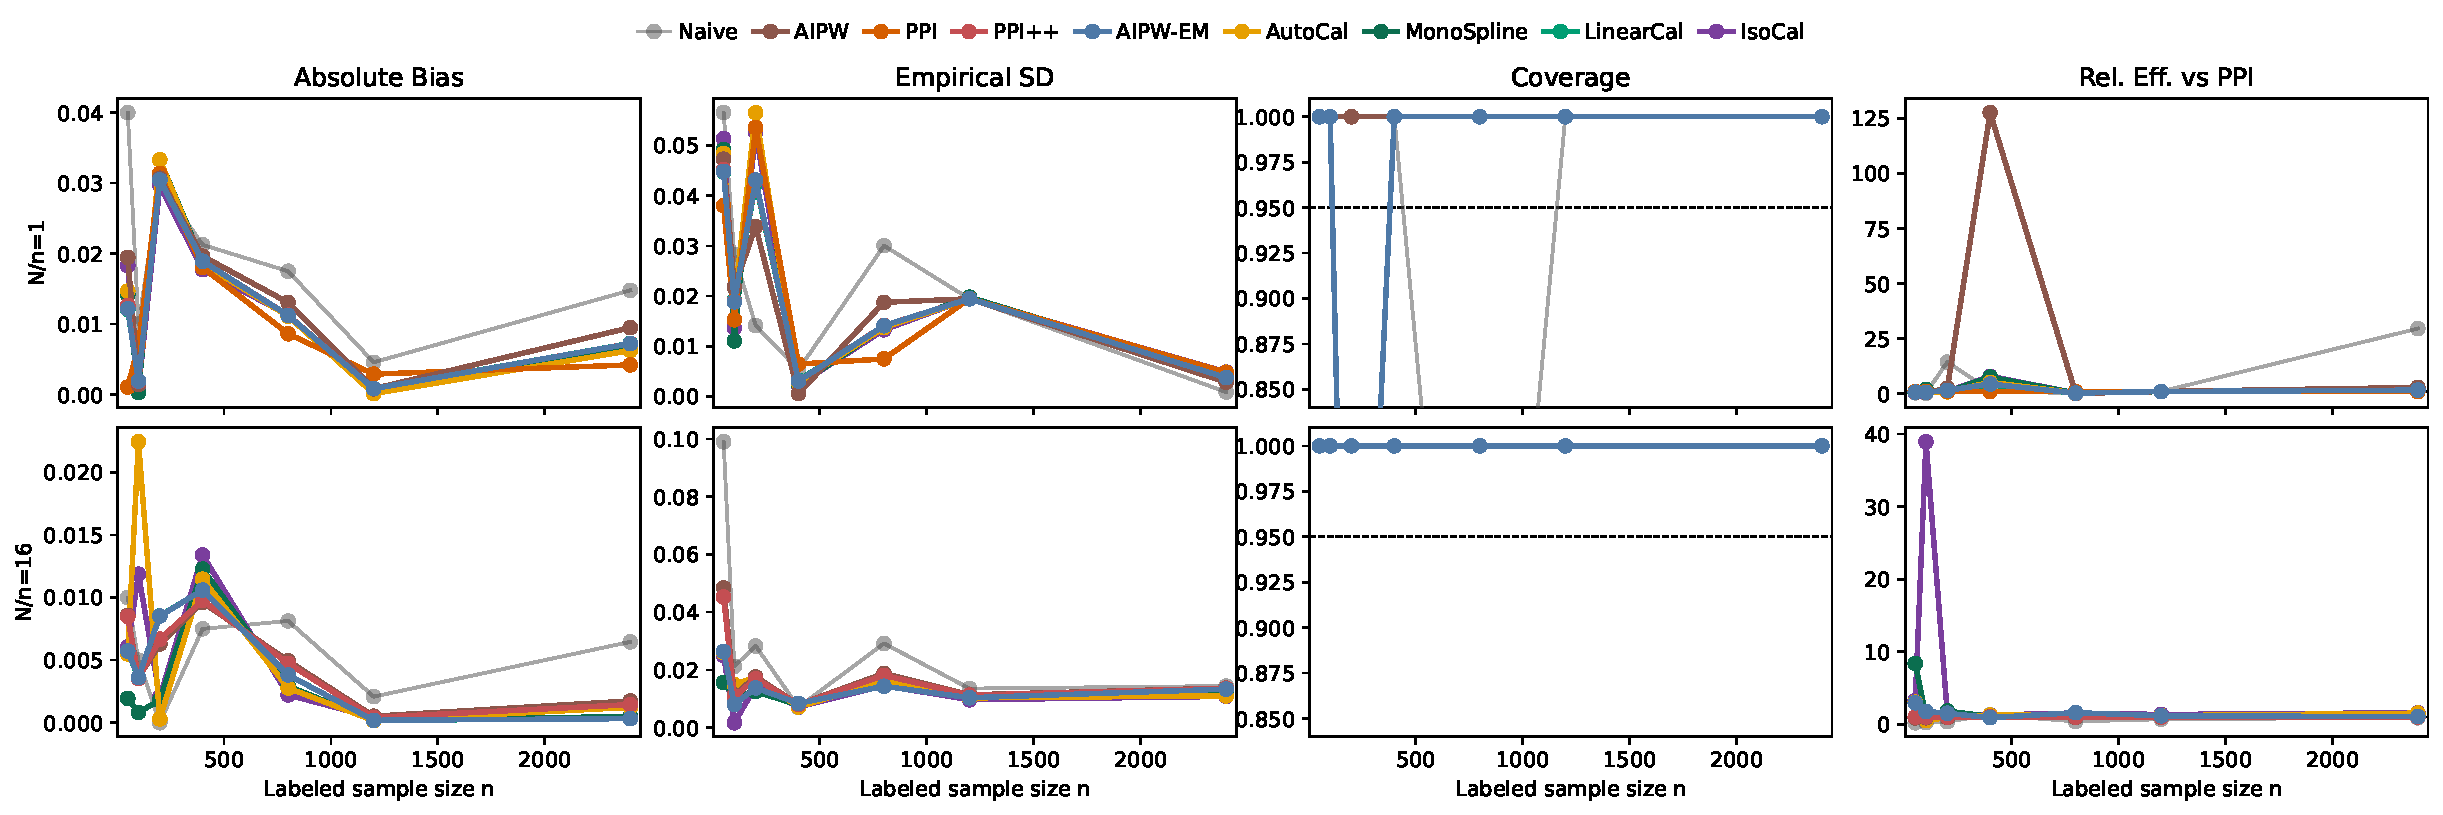
\includegraphics[width=\textwidth]{assets/sim_fig_main.pdf}
\caption{Synthetic simulation study with a poorly calibrated score. The top row shows the balanced case \(N/n=1\), and the bottom row shows the large-unlabeled case \(N/n=16\). All estimators had negligible bias relative to their standard errors, so we omit the bias panel. The three columns report empirical Monte Carlo standard deviation, coverage, and relative efficiency versus PPI. Lower standard deviation is better, coverage closer to the nominal \(0.95\) is better, and relative efficiency above \(1\) indicates an estimator is more efficient than PPI (so higher is better).}
\label{fig:simulation-rmse}
\end{figure}


Figure \ref{fig:simulation-rmse} isolates the main mechanism. All score-based AIPW-type estimators are essentially unbiased, so the key comparison is efficiency: AIPW improves on PPI, and calibration helps when the score is genuinely miscalibrated. At \(n=400\) and \(N/n=16\), the calibrated methods reduce RMSE from about \(0.0172\) for PPI to about \(0.0164\); by \(n=1200\) in the same regime, RMSE is about \(0.0087\) for \textsc{AutoCal}, \textsc{MonoSpline}, and \textsc{IsoCal}, compared with \(0.0092\) for PPI. The PPI++ comparison is most revealing when the unlabeled sample is large: \textsc{AIPW-EM} remains essentially indistinguishable from \texttt{LinearCal}, whereas clipped PPI++ falls back toward plain PPI. Averaging over the poorly calibrated designs with \(N/n=16\), RMSE is about \(0.0196\) for \textsc{AIPW-EM} and \texttt{LinearCal}, versus \(0.0208\) for PPI++, reflecting the fact that the official \texttt{ppi\_py} implementation clips the optimized scaling coefficient to \([0,1]\), whereas \textsc{AIPW-EM} does not. \textsc{AutoCal} remains close to the best fixed score-based option, and \texttt{MonoSpline} provides a smooth monotone alternative that is usually close to isotonic calibration.


\subsection{Empirical Illustration}
\label{sec:empirical}

We evaluate the proposed calibration-based estimators on the mean-estimation benchmarks used in the original experiments of \citet{ppi2023,angelopoulos2023ppi}, as provided in the \texttt{ppi\_py} package. We use the same \texttt{ppi\_py} datasets and labeled-sample-size grids, repeatedly split each fully labeled benchmark into labeled and unlabeled subsets, evaluate all estimators on the same split, and treat the full-sample mean as ground truth.\footnote{Because repeated sample splits of a fixed finite benchmark dataset are not i.i.d.\ draws from a superpopulation, asymptotic Wald confidence intervals can exhibit either undercoverage or overcoverage. This is not specific to our calibration extensions, but is a feature of evaluating Wald-type intervals under finite-population resampling.} The current draft summaries average over 500 random splits at each \(n\). We report the official \texttt{forest}, \texttt{galaxies}, and \texttt{census\_income} benchmarks and focus the main text on the primary comparator set already shown in the figure: PPI, AIPW, PPI++, \textsc{AIPW-EM}, \texttt{LinearCal}, and \texttt{AutoCal}. Appendix~\ref{app:empirical} gives the fuller method inventory, calibration-specific comparisons, and dataset-by-regime summary.


\begin{figure}[htb]
\centering
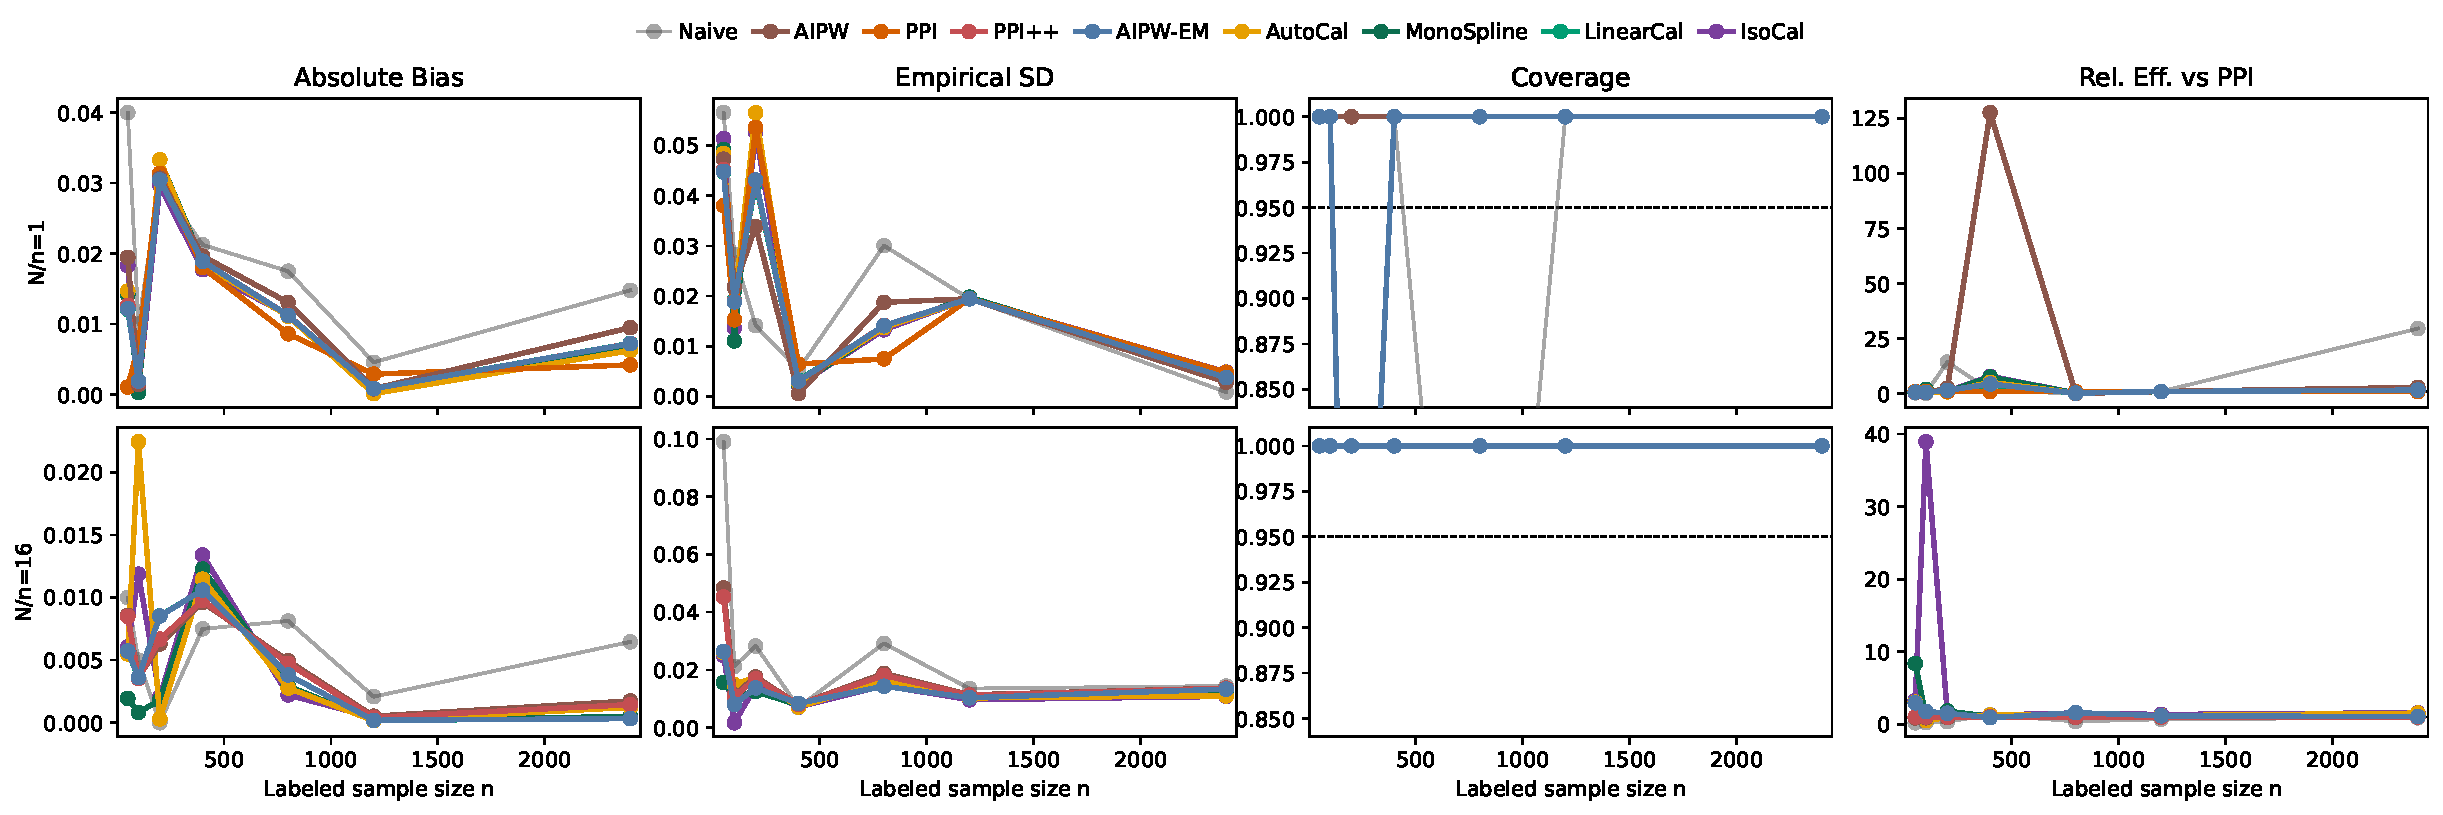
\includegraphics[width=\textwidth]{assets/sim_fig_main.pdf}
\caption{Main-text benchmark summary for the reproduced \texttt{ppi\_py} datasets. Panels report normalized MSE relative to PPI, relative efficiency versus PPI, and coverage for the main comparator set.}
\label{fig:ppi-main}
\end{figure}

Figure~\ref{fig:ppi-main} shows the same pattern on the reproduced benchmarks. AIPW is the stronger raw-score baseline, with PPI competitive only when the unlabeled sample is extremely large. The clearest calibration gain appears in \texttt{census\_income}, where \texttt{LinearCal} performs best on average, and the appendix comparison in \cref{fig:ppi-calibration-appendix} shows that \texttt{IsoCal} and \texttt{MonoSpline} remain broadly competitive without changing the main ranking. The added efficiency-maximization baseline also sharpens the comparison with PPI++: across the 30 dataset-size cells in \cref{fig:ppi-main}, \textsc{AIPW-EM} has lower MSE than clipped PPI++ in 29 and is nearly tied with \texttt{LinearCal}. Averaged across all cells, the mean MSE is about \(4.75\times 10^6\) for \textsc{AIPW-EM}, \(4.75\times 10^6\) for \texttt{LinearCal}, and \(5.03\times 10^6\) for PPI++, with essentially identical coverage near \(0.919\). This mirrors the simulations: once the empirical efficiency-maximization step is left unclipped, its finite-sample behavior moves much closer to \texttt{LinearCal}. \texttt{AutoCal} serves as a practical hedge that tends to remain close to the best fixed score-based method. Appendix~\ref{app:empirical} provides a fuller summary by dataset and regime.

\subsection{LLM evaluation benchmark}
\label{sec:llm-benchmark}

We now turn to a practical LLM-evaluation setting in which we apply the same comparison hierarchy to real public model outputs, public evaluator scores, and public labels. The first track uses PPE Human Preference V1 \citep{frick2025evaluate}, where the estimand for each target model is its human win rate across prompt--response comparisons, counting ties as half-wins. The second track uses a PPE correctness suite \citep{frick2025evaluate} built from MMLU-Pro \citep{wang2024mmlupro}, MATH \citep{hendrycksmath2021}, GPQA \citep{rein2024gpqa}, IFEval \citep{zhou2023instructionfollowing}, and MBPP+ \citep{liu2023evalplus}, where each unit consists of a sampled conflict pair from the same generator model and the estimand is the correctness probability of the first answer in the pair. In both tracks, the prompts, outputs, judgments, and evaluator scores are real; only the labeled/unlabeled split is rerandomized. Across 200 repeated splits, we compare labeled-only estimation with raw PPI and AIPW, their efficiency-maximized variants, and the calibration-based estimators from our main experiments.




\IfFileExists{assets/fig_llm_eval_main.pdf}{
\begin{figure}[htb]
\centering
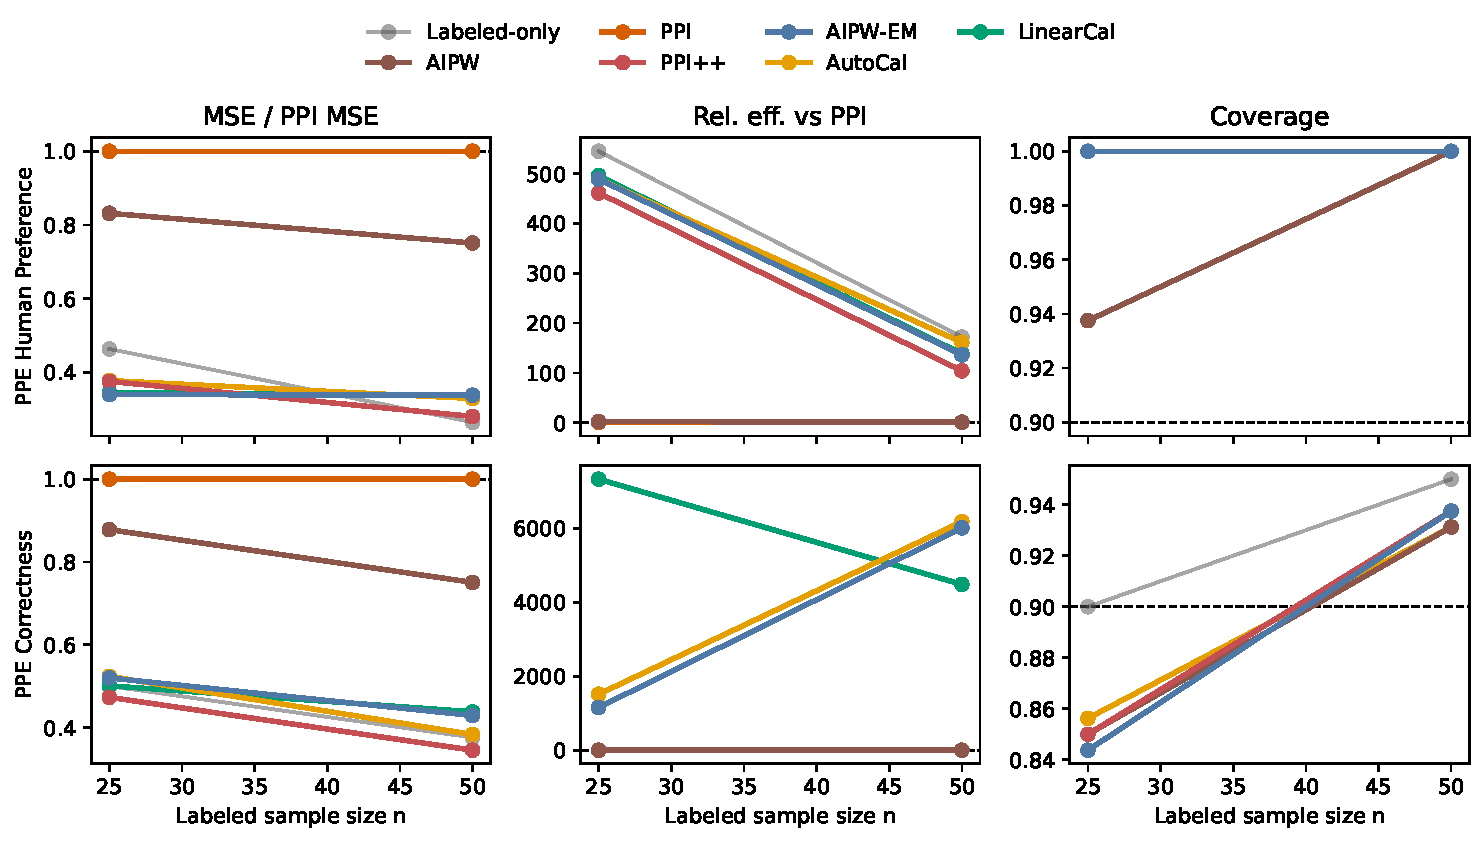
\includegraphics[width=\textwidth]{assets/fig_llm_eval_main.pdf}
\caption{PPE-centered LLM-evaluation benchmark. Panels report normalized MSE relative to PPI, relative efficiency versus labeled-only, and coverage after macro-averaging across the public PPE evaluator models. We omit RewardBench from the main-text figure until its separate robustness run completes cleanly.}
\label{fig:llm-eval-main}
\end{figure}
}{}

\IfFileExists{assets/table_llm_summary.tex}{
\begin{table}[htb]
\centering
\small
\resizebox{\textwidth}{!}{\begin{tabular}{lllrccc}
\toprule
Track & $n$ & Estimator & MSE / PPI & RelEff / PPI & Coverage & Label savings \\
\midrule
PPE Correctness & 25 & AIPW & 0.878 & 1.367 & 0.850 & 0.113 \\
PPE Correctness & 25 & AIPW-EM & 0.520 & 1157.062 & 0.844 & 0.202 \\
PPE Correctness & 25 & AutoCal & 0.524 & 1515.978 & 0.856 & 0.210 \\
PPE Correctness & 25 & Labeled-only & 0.500 & inf & 0.900 & 0.000 \\
PPE Correctness & 25 & IsoCal & 0.452 & 11575.686 & 0.875 & 0.194 \\
PPE Correctness & 25 & LinearCal & 0.501 & 7335.829 & 0.850 & 0.208 \\
PPE Correctness & 25 & MonoSpline & 0.481 & 1041.054 & 0.844 & 0.228 \\
PPE Correctness & 25 & Platt & 0.498 & 12288.149 & 0.863 & 0.241 \\
PPE Correctness & 25 & PPI & 1.000 & 1.000 & 0.850 & 0.110 \\
PPE Correctness & 25 & PPI++ & 0.473 & inf & 0.850 & 0.132 \\
PPE Correctness & 50 & AIPW & 0.751 & 1.769 & 0.931 & 0.112 \\
PPE Correctness & 50 & AIPW-EM & 0.429 & 6018.106 & 0.938 & 0.220 \\
PPE Correctness & 50 & AutoCal & 0.383 & 6184.299 & 0.931 & 0.205 \\
PPE Correctness & 50 & Labeled-only & 0.376 & inf & 0.950 & 0.000 \\
PPE Correctness & 50 & IsoCal & 0.408 & inf & 0.925 & 0.240 \\
PPE Correctness & 50 & LinearCal & 0.438 & 4487.608 & 0.938 & 0.217 \\
PPE Correctness & 50 & MonoSpline & 0.425 & 148597065531295156473430016.000 & 0.919 & 0.239 \\
PPE Correctness & 50 & Platt & 0.426 & 7455.383 & 0.931 & 0.225 \\
PPE Correctness & 50 & PPI & 1.000 & 1.000 & 0.938 & 0.102 \\
PPE Correctness & 50 & PPI++ & 0.345 & inf & 0.938 & 0.192 \\
PPE Human Preference & 25 & AIPW & 0.832 & 2.390 & 0.938 & 0.141 \\
PPE Human Preference & 25 & AIPW-EM & 0.340 & 489.182 & 1.000 & 0.177 \\
PPE Human Preference & 25 & AutoCal & 0.378 & 488.899 & 1.000 & 0.176 \\
PPE Human Preference & 25 & Labeled-only & 0.464 & 545.093 & 1.000 & 0.000 \\
PPE Human Preference & 25 & IsoCal & 0.369 & 427.847 & 1.000 & 0.172 \\
PPE Human Preference & 25 & LinearCal & 0.345 & 495.939 & 1.000 & 0.173 \\
PPE Human Preference & 25 & MonoSpline & 0.338 & 293.144 & 1.000 & 0.228 \\
PPE Human Preference & 25 & PPI & 1.000 & 1.000 & 0.938 & 0.140 \\
PPE Human Preference & 25 & PPI++ & 0.376 & 461.364 & 1.000 & 0.145 \\
PPE Human Preference & 50 & AIPW & 0.751 & 1.378 & 1.000 & 0.010 \\
PPE Human Preference & 50 & AIPW-EM & 0.338 & 136.356 & 1.000 & 0.138 \\
PPE Human Preference & 50 & AutoCal & 0.329 & 161.658 & 1.000 & 0.148 \\
PPE Human Preference & 50 & Labeled-only & 0.265 & 172.214 & 1.000 & 0.000 \\
PPE Human Preference & 50 & IsoCal & 0.446 & 152.657 & 1.000 & 0.087 \\
PPE Human Preference & 50 & LinearCal & 0.335 & 138.599 & 1.000 & 0.140 \\
PPE Human Preference & 50 & MonoSpline & 0.350 & 153.849 & 1.000 & 0.042 \\
PPE Human Preference & 50 & PPI & 1.000 & 1.000 & 1.000 & 0.012 \\
PPE Human Preference & 50 & PPI++ & 0.280 & 104.304 & 1.000 & 0.037 \\
\bottomrule
\end{tabular}
}
\caption{Compact PPE-only numerical summary at \(n\in\{100,400\}\), restricted to the headline estimators from the main-text discussion. Each row reports normalized MSE relative to PPI, implied label savings relative to labeled-only, and coverage for one estimator-track pair. The fuller estimator comparison appears in Appendix~\ref{tab:llm-eval-summary-full}.}
\label{tab:llm-eval-summary}
\end{table}
}{}

Two messages stand out. First, naive use of the proxy can fail badly. Raw AIPW is again the stronger raw-score baseline, but even AIPW can perform dramatically worse than labeled-only estimation when the reward-model margin is poorly scaled. On PPE Human at \(n=100\), raw PPI and raw AIPW have MSE \(0.495\) and \(0.440\), compared with \(0.001425\) for labeled-only and \(0.001391\) for \texttt{LinearCal}. On PPE Correctness at \(n=100\), the corresponding MSEs are \(0.534\), \(0.353\), \(0.002010\), and \(0.001813\). These estimators remain valid first-order corrections, but the additional proxy term can inflate variance enough that labeled-only estimation is much safer.

Second, calibration makes the same evaluator scores practically useful. \texttt{LinearCal} is the strongest and most stable method overall, with \texttt{AutoCal} close behind. On PPE Human, \texttt{LinearCal} is best from \(n=50\) onward, improving on labeled-only from \(0.001425\) to \(0.001391\) at \(n=100\) and from \(0.000286\) to \(0.000278\) at \(n=400\), corresponding to modest label savings of about \(2.5\%\) to \(3.1\%\). On PPE Correctness, the gains are clearer: \texttt{LinearCal} is best at every budget, improving from \(0.002010\) to \(0.001813\) at \(n=100\) and from \(0.000248\) to \(0.000222\) at \(n=400\), corresponding to about \(7.5\%\) to \(10.5\%\) label savings. The more flexible calibration rules are also competitive once the labeled sample is moderately large. On PPE Human, \texttt{AutoCal} and \texttt{MonoSpline} remain in the \(2.5\%\) to \(2.8\%\) label-savings range from \(n=100\) to \(n=400\); on PPE Correctness, they remain in roughly the \(9\%\) to \(10\%\) range over the same budgets. \texttt{MonoSpline} therefore substantially improves on raw PPI and raw AIPW and is usually competitive with PPI++ and \textsc{AIPW-EM}, though it remains slightly less stable than \texttt{LinearCal}. The evaluator-specific appendix breakdown (\Cref{fig:llm-eval-by-evaluator}) shows that the most extreme raw-proxy failures are driven by evaluators such as Skywork and Athene, whereas ArmoRM is much more benign. Calibration also improves the downstream ranking task induced by PPE Human. Raw PPI and raw AIPW recover the model ordering poorly, whereas calibrated and efficiency-maximized methods recover it well. At \(n=200\), \texttt{AutoCal} attains the highest average Spearman correlation, about \(0.905\); at \(n=400\), \texttt{LinearCal} achieves the best overall ranking quality, with Spearman correlation about \(0.941\) and top-1 identification rate about \(0.646\). We therefore view calibration not as a marginal efficiency tweak, but as the step that makes cheap public LLM evaluators safe enough to use in practice; see Appendix~\ref{app:llm-ranking}.

\section{Conclusion and closing remarks}

We introduced \emph{Calibrated Prediction-Powered Inference}, a simple framework for semisupervised mean estimation based on three steps: fit a prediction score, calibrate it on the labeled sample, and average the calibrated predictions over the pooled covariate sample. This simple plug-in procedure fits naturally within the broader literature on semiparametric debiasing and can be viewed as a semisupervised specialization of calibrated debiased machine learning \citep{van2024automatic}.

Our results highlight a simple message. Calibration can improve semisupervised efficiency without retraining the original model, and isotonic calibration can \emph{calibeat} the original score and simpler post-processing rules at first order. At the same time, once the score has been isotonicly calibrated, further post-processing of that fitted score brings no additional first-order gain. Empirically, this suggests a transparent and practical workflow: when the original score is already well calibrated, calibration changes little, whereas under meaningful miscalibration, even simple linear or monotone calibration can improve efficiency while preserving a transparent plug-in form.


\textbf{Positioning PPI within existing semiparametric methods.}
More broadly, our results clarify that recent prediction-powered inference methods can be understood within the standard semiparametric, debiased machine-learning, and flexible covariate-adjustment toolkit for randomized trials and missing-at-random settings. In particular, we show that PPI++ is an AIPW estimator with empirical efficiency maximization \citep{rubin2008empirical} and is first-order equivalent to linear calibration and classical prognostic-score regression adjustment \citep{hansen2008prognostic,lin2013agnostic,schuler2022increasing}. It is therefore closely related to randomized-trial approaches that learn prognostic scores from larger historical, external-control, or auxiliary data sets and then use them for regression adjustment in smaller trials \citep{hansen2008prognostic,moore2009covariate,rosenblum2009using,benkeser2021improving,hojbjerre2025powering}. This perspective suggests that semisupervised inference may benefit from closer integration with the broader missing-data, causal-inference, and debiased machine-learning literatures. These lines of work study closely related versions of the same core problem: how to use flexible regression adjustment learned from auxiliary data while retaining valid inference for the target parameter. Further progress may therefore come from translational work across them, especially by adapting tools developed for randomized trials and missing-at-random settings to semisupervised problems \citep{petersen2014causal,dang2023causal,ho2023current,smith2023application,ho2024examples}.

 


\textbf{Beyond mean estimation.}
These connections extend well beyond the semisupervised mean-estimation setting considered here. For example, when missingness affects both outcomes and covariates and may depend on observed covariates and outcomes, as well as in extensions to right-censored time-to-event outcomes and longitudinal settings, existing semiparametric methods often provide natural starting points and can frequently be adapted to these settings \citep{robins1994estimation,vanderlaanunified,bang2005doubly,moore2009increasing,rose2011targeted,van2018targeted}. More generally, M-estimation and estimating-equation approaches for missing-at-random problems are well developed \citep{robins1994estimation,vanderlaanunified,DoubleML}. When missingness depends on unobserved outcomes even after conditioning on observed data, however, naively pooling labeled and unlabeled data can bias estimation. There is substantial work on combining gold-standard and potentially biased auxiliary data more safely using semiparametric and machine-learning tools \citep{kallus2018removing,rosenman2025methods,dang2025experiment,van2026adaptive}. Similarly, when the unlabeled sample is selected in a data-dependent way, the problem becomes closely related to adaptive and selectively sampled designs, including two-phase and informative sampling \citep{van2008construction,chow2008adaptive,rose2011targeted,malenica2021adaptive,zrnic2024active,zhang2025efficient,liu2025robust}. Extending these broader missing-data and adaptive-sampling ideas to modern semisupervised inference is therefore a natural direction for future work.

  
 
 

\textbf{Towards conditional prediction-powered inference} There is already a well-developed literature on machine-learning-assisted estimation of local and conditional regression targets, including regression functions, dose-response curves, and conditional average treatment effects, which can be used to extend inference beyond marginal mean estimation \citep{rubin2006doubly,diaz2013targeted,kennedy2017non,bibaut2017data,van2018cv,westling2020causal,chernozhukov2022debiased,kennedy2023towards,foster2023orthogonal,chernozhukov2023simple,luedtke2024one,chernozhukov2024conditional,butzin2024highly,zhang2025constructing,gu2024local,sui2026prediction}. In particular, kernel-regression-based \citep{bibaut2017data} and isotonic-regression-based \citep{westling2020unified} inference can be used for conditional PPI with AIPW-score-based pseudo-outcomes, as in \citet{van2003unified,rubin2006doubly,kennedy2017non}, or more generally through influence functions and Neyman-orthogonal losses \citep{bibaut2017data,chernozhukov2024conditional}. The key idea is that locally smoothed conditional targets are amenable to influence-function-based bias correction, after which inference follows from a triangular-array central limit theorem applied to estimators of a sequence of approximating parameters \citep{bibaut2017data,chernozhukov2022debiased,luedtke2024one,chernozhukov2024conditional}. In the prediction-powered setting, a natural approach is to apply kernel regression to AIPW-style pseudo-outcomes for missing-data problems, following \citet{rubin2006doubly}, \citet{takatsu2025debiased}, and \citet{bibaut2017data,kennedy2017non,chernozhukov2024conditional}.
 
 
 

 


\textbf{Calibration for general loss functions.} While we focus on calibration of regression functions and inference on means, the ideas here may extend to broader supervised learning problems defined through loss minimization, such as median and quantile regression \citep{rosenblum2009using,noarov2023statistical,jung2021moment,roth2022uncertain,whitehouse2024orthogonal}. They also extend to continuous linear functionals of a regression function or M-estimand through calibrated DML \citep{van2024automatic,van2025automatic}. More generally, when the target parameter is defined by a moment equation, as in M-estimation, one could debias or calibrate the associated augmented moment equation \citep{vanderlaanunified,DoubleML}; see Appendix~\ref{appendix::momentgeneral} and \citet{ji2025predictions}. A practical challenge in this setting is that the augmented loss may be nonconvex or may require separate debiasing at each parameter value, which can complicate optimization. In such cases, a more practical alternative may be a multiaccuracy-style adjustment rather than explicit augmentation or calibration, as in the Efficient Plug-in Learning framework of \citet{van2024combining}, which addresses this issue for nonconvex Neyman-orthogonal loss functions \citep{foster2023orthogonal}.

\bibliographystyle{plainnat}
\bibliography{references}

 


 


\appendix


\tableofcontents

 \section{Additional background on semiparametric statistics}
  \label{section::plugin}




The next result shows that the efficient choice in  Proposition \ref{prop:aipw-class}  is not merely optimal within the AIPW class. In fact, every regular estimator\footnote{Informally, a regular estimator is one whose large-sample behavior remains stable under small changes in the data-generating distribution \citep{van2000asymptotic}.} in the unrestricted two-sample model is asymptotically equivalent to \(\widehat\psi(f)\) for some score function \(f\). Thus, the AIPW family characterizes the full class of regular estimators at first order in this model.

\begin{proposition}[Characterization of regular estimators]
\label{prop:if-class}
Under \cref{assump:design}, a mean-zero pair \((D^L,D^U)\) is the influence pair of a regular estimator of \(\psi_0\) in the unrestricted two-sample model if and only if there exists a function \(f_0:\mathcal X\to\R\) with finite second moment, potentially depending on \(P_0\), such that
\[
(D^L,D^U)=(D_{f_0}^L,D_{f_0}^U),
\]
where \(D_f^L\) and \(D_f^U\) are given in Proposition \ref{prop:aipw-class}. Equivalently, for every regular estimator \(\widehat\psi^\dagger\), there exists such an \(f_0\) for which
\[
\widehat\psi^\dagger-\widehat\psi(f_0)=o_p(M^{-1/2}).
\]
\end{proposition}
 

This characterization shows that the AIPW class is the relevant first-order benchmark in this model. The next remark illustrates that several estimators not always written in AIPW form---including regression adjustment, balancing-weight adjustment, and TMLE---can nonetheless be viewed as finite-sample or asymptotic equivalents of AIPW estimators \citep{rotnitzky2025note,van2006targeted}, while sometimes offering better finite-sample performance \citep{porter2011relative,jin2026prognostic,van2025automatic}.

 


\begin{remark}[Plug-in approaches to bias correction and TMLE]
    
 
 
  \textbf{Regression plug-in estimators.} A particularly simple member of this first-order class is obtained through plug-in regression adjustment \citep{scharfstein1999adjusting,van2006targeted,rosenblum2009using,rotnitzky2025note}. Let
\[
m_n(X)=\hat a_{\mathrm{lin}}\,m(X)+\hat b_{\mathrm{lin}},
\qquad
(\hat a_{\mathrm{lin}},\hat b_{\mathrm{lin}})
=
\arg\min_{a,b}\sum_{i=1}^n \{Y_i-a\,m(X_i)-b\}^2.
\]
The corresponding plug-in estimator is
\[
\rho_n \Pl\{m_n(X)\} + (1-\rho_n)\Pu\{m_n(\widetilde X)\}.
\]
For any \(\lambda\in\mathbb{R}\), this estimator also admits the AIPW representation
\[
\rho_n \Pl\{m_n(X)\}
+
(1-\rho_n)\Pu\{m_n(\widetilde X)\}
+
\lambda \Pl\bigl[Y-m_n(X)\bigr],
\]
because the augmentation term \(\Pl\{Y-m_n(X)\}\) is zero by the least-squares normal equations. Thus, when \(m_n\) converges to the best linear predictor of \(Y\) given \(m(X)\), this plug-in estimator is typically at least as efficient as \(\widehat{\psi}_{\mathrm{AIPW}}\) and \(\widehat{\psi}_{\mathrm{PPI}}\), since it corresponds to an influence function with smaller or equal variance.

\textbf{Balancing-weight estimators.} The same estimator can also be written in terms of balancing weights. Let \(w_n(X)=\hat a_{\mathrm{bal}}+\hat b_{\mathrm{bal}}\,m(X)\) be affine weights that balance \((1,m(X))\), in the sense that
\[
\Pl\{w_n(X)\}=1
\quad\text{and}\quad
\Pl\bigl[m(X)w_n(X)\bigr]
=
\rho_n \Pl\{m(X)\}+(1-\rho_n)\Pu\{m(\widetilde X)\}.
\]
Then the corresponding balancing-weight estimator satisfies
\[
\Pl\bigl\{w_n(X)Y\bigr\}
=
\rho_n \Pl\{m(X)\}
+
(1-\rho_n)\Pu\{m(\widetilde X)\}
+
\Pl\bigl[w_n(X)\{Y-m(X)\}\bigr].
\]
In fact, the plug-in and balancing-weight estimators are algebraically equivalent \citep{chattopadhyay2023implied,bruns2025augmented}:
\[
\Pl\bigl\{w_n(X)Y\bigr\}
=
\rho_n \Pl\{m_n(X)\}
+
(1-\rho_n)\Pu\{m_n(\widetilde X)\}.
\]

\textbf{TMLE.} More broadly, such debiased plug-in estimators can be viewed as instances of TMLE \citep{van2006targeted,vanderLaanRose2011,hojbjerre2026within}, a general framework for constructing plug-in estimators that are debiased and, in many cases, efficient by updating nuisance components to remove first-order bias. In the present setting, either the weights or the regression model are updated so that the corresponding augmentation term vanishes. In weighting-based TMLE, the update balances on the prediction model \(m(X)\) (e.g., \citealt{hejazi2023revisiting}); one may either include the known weight \(1/\rho_n\) as an offset or balance on the intercept as well. In regression-based TMLE, the prediction model \(m(X)\) may be included either as a covariate or as an offset (e.g., \citealt{lendle2015balancing}), and the intercept adjustment accounts for the known inverse missingness-probability weight \(1/\rho_n\). The specific targeting step is ultimately a practical choice, provided it solves the relevant estimating equation and removes the augmentation term; different choices may also yield additional benefits, such as further bias reduction or doubly robust inference \citep{van2014targeted,carone2014higher,diaz2017doubly,benkeser2017doubly,van2021higher, van2024automatic}.
 \end{remark}


\section{Constructing confidence intervals via the bootstrap}

 

Confidence intervals may be constructed using the standard Wald approximation from Corollary \ref{cor:normal}, namely
\[
\widehat{\psi}_{\mathrm{iso}}
\pm
z_{1-\alpha/2}\,\frac{\hat\sigma}{\sqrt{n+N}}.
\]
As an alternative, one may use the nonparametric bootstrap and refit the isotonic calibration step within each bootstrap replicate, as proposed and theoretically studied by \citet{van2024automatic}; see also \citet{tang2024consistency}. This avoids direct estimation of the influence-function variance and automatically propagates uncertainty from estimation of the calibration map.  


For each bootstrap replicate \(b=1,\dots,B\), we sample with replacement from the labeled observations \(\{(X_i,Y_i)\}_{i=1}^n\) and, independently, from the unlabeled observations \(\{\widetilde X_j\}_{j=1}^N\), obtaining bootstrap samples
\[
\{(X_i^{*(b)},Y_i^{*(b)})\}_{i=1}^n,
\qquad
\{\widetilde X_j^{*(b)}\}_{j=1}^N.
\]
We then refit the isotonic calibrator on the bootstrap labeled sample:
\begin{align*}
\hat f^{*(b)}
\in
\arg\min_{f \in \mathcal F_{\mathrm{iso}}}
\sum_{i=1}^n
\bigl\{Y_i^{*(b)} - f(\mhat(X_i^{*(b)}))\bigr\}^2,
\end{align*}
and define
\[
m_{\mathrm{iso}}^{*(b)}(X):=\hat f^{*(b)}\{\mhat(X)\}.
\]
The corresponding bootstrap replicate of the estimator is
\[
\widehat{\psi}_{\mathrm{iso}}^{*(b)}
:=
\frac{1}{n+N}\left\{
\sum_{i=1}^n m_{\mathrm{iso}}^{*(b)}(X_i^{*(b)})
+
\sum_{j=1}^N m_{\mathrm{iso}}^{*(b)}(\widetilde X_j^{*(b)})
\right\}.
\]

After computing \(B\) bootstrap replicates, one may form a percentile interval using the empirical \(\alpha/2\) and \(1-\alpha/2\) quantiles of
\[
\bigl\{\widehat{\psi}_{\mathrm{iso}}^{*(b)}\bigr\}_{b=1}^B.
\]
Alternatively, one may use the bootstrap standard error
\[
\widehat{\sigma}_{\mathrm{boot}}^2
:=
\frac{1}{B-1}\sum_{b=1}^B
\left(\widehat{\psi}_{\mathrm{iso}}^{*(b)}-\bar{\psi}_{\mathrm{iso}}^\star\right)^2,
\qquad
\bar{\psi}_{\mathrm{iso}}^\star
:=
\frac{1}{B}\sum_{b=1}^B \widehat{\psi}_{\mathrm{iso}}^{*(b)},
\]
and report the normal-approximation interval
\[
\widehat{\psi}_{\mathrm{iso}}
\pm
z_{1-\alpha/2}\,\widehat{\sigma}_{\mathrm{boot}}.
\]

The key implementation detail is that the isotonic regression step must be refit within each bootstrap replicate rather than held fixed. Otherwise, the resulting interval does not reflect uncertainty from estimation of the calibration map.




\section{Additional remarks}

\label{appendix:remarks}


\begin{remark}[Empirical efficiency maximization as a learning objective]
We  review \cite{rubin2008empirical}. The empirical variance criterion from Section~\ref{sec:effreview},
\[
\sigma_n^2(f)
:=
\rho_n \Pl\left[\left\{f(X)-\widehat{\psi}(f)+\rho_n^{-1}(Y-f(X))\right\}^2\right]
+
(1-\rho_n)\Pu\left[\left\{f(\widetilde X)-\widehat{\psi}(f)\right\}^2\right],
\]
is not tied to the one-dimensional scaling class \(\{\lambda m(X):\lambda\in\R\}\). For any candidate class \(\mathcal G\subset L^2(\Px)\), one may instead define
\[
\hat f \in \arg\min_{f\in\mathcal G}\sigma_n^2(f),
\qquad
\widehat\psi_{\mathrm{eem}}:=\widehat\psi(\hat f),
\]
so empirical efficiency maximization learns the augmentation \(f(X)\) directly.

At the population level, let
\[
V(f):=\rhozero\Var[D_f^L(X,Y)]+(1-\rhozero)\Var[D_f^U(\widetilde X)]
\]
denote the asymptotic variance of \(\widehat\psi(f)\). Using Proposition \ref{prop:aipw-class},
\[
V(f)
=
\Var[Y]+\frac{1-\rhozero}{\rhozero}\Var[Y-f(X)].
\]
Equivalently, with \(\tilde f(X):=f(X)-\E_{\Px}[f(X)]+\psi_0\),
\[
V(f)
=
\Var[Y]+\frac{1-\rhozero}{\rhozero}\E\bigl[(Y-\tilde f(X))^2\bigr].
\]
Thus the efficiency-optimal choice is the \(L^2(\Px)\)-projection of \(\mu_0\) onto the normalized class \(\{\tilde f:f\in\mathcal G\}\). If \(\mathcal G\) is closed under additive constants, then minimizing \(V(f)\) is equivalent to ordinary least-squares regression of \(Y\) on \(X\) over \(\mathcal G\). In particular, rather than optimizing the empirical efficiency criterion \(\sigma_n^2(f)\) directly, one can equivalently optimize the usual empirical mean-squared-error objective on the labeled sample.


This makes richer efficiency-maximizing classes immediate. For example, if \(\mathcal G=\{b+h:h\in\mathcal H,\ b\in\R\}\) for an RKHS \(\mathcal H\) with kernel \(K\), then a penalized version of empirical efficiency maximization is
\[
(\hat b_\lambda,\hat h_\lambda)
\in
\arg\min_{b\in\R,\ h\in\mathcal H}
\left\{
\Pl\bigl[(Y-b-h(X))^2\bigr]+\lambda\|h\|_{\mathcal H}^2
\right\},
\]
which is just kernel ridge regression on the labeled sample, up to the irrelevant additive constant in the variance criterion. By the representer theorem,
\[
\hat h_\lambda(\cdot)=\sum_{i=1}^n \hat\alpha_i K(X_i,\cdot),
\]
and, after centering the kernel or including the intercept explicitly,
\[
\hat\alpha=(K_n+n\lambda I_n)^{-1}(Y-\hat b_\lambda \mathbf 1_n).
\]
Plugging \(\hat f_\lambda=\hat b_\lambda+\hat h_\lambda\) into \(\widehat\psi(\hat f_\lambda)\) yields the corresponding efficiency-maximized AIPW estimator.

For tuning and class selection, it is preferable to evaluate the same criterion out of fold. One may split the labeled sample into folds, fit \(f^{-k}\) on the training part of fold \(k\), compute the held-out criterion \(\sigma_{n,k}^2(f^{-k})\), and average over folds. The selected class or tuning parameter can then be used in a cross-fitted or cross-averaged AIPW estimator. This gives a direct cross-validated empirical efficiency objective for choosing among classes such as linear, spline, isotonic, or RKHS-based regressors while preserving the usual sample-splitting protection against in-sample overfitting.
\end{remark}



\begin{remark}[Shrinkage via Venn--Abers]
When the labeled sample is small, isotonic calibration may be unstable. A natural alternative is Venn--Abers calibration, originally introduced for binary classification \citep{vovk2012venn}; see \cite{van2024self, van2025venn} for generalized versions beyond the binary setting. Assume \(Y \in [0,1]\), or rescale otherwise. For each \(x\), augment the labeled calibration sample with the hypothetical point \((\mhat(x),y)\) for \(y \in \{0,1\}\), fit the resulting isotonic calibrators \(f_n^{(x,0)}\) and \(f_n^{(x,1)}\), and form the interval-valued prediction
\[
\bigl[f_n^{(x,0)}\{\mhat(x)\},\, f_n^{(x,1)}\{\mhat(x)\}\bigr].
\]
Following \cite{vovk2012venn}, one may convert this interval to a point prediction by shrinking its midpoint toward the (unadjusted) AIPW estimator:
\[
m_{n,\mathrm{VA}}^\star(x)
:=
m_{n,\mathrm{mid}}^\star(x)
+
\bigl\{f_n^{(x,1)}\{\mhat(x)\}-f_n^{(x,0)}\{\mhat(x)\}\bigr\}
\bigl\{\widehat\psi_{AIPW}-m_{n,\mathrm{mid}}^\star(x)\bigr\},
\]
where
\[
\begin{aligned}
m_{n,\mathrm{mid}}^\star(x)
&:=
\frac{f_n^{(x,1)}\{\mhat(x)\}+f_n^{(x,0)}\{\mhat(x)\}}{2}.
\end{aligned}
\]
Since the shrinkage magnitude is proportional to the width of the Venn--Abers interval, this construction can be more stable than plain isotonic calibration in small samples.
\end{remark}
 

\begin{remark}[Relation between linear calibration, PPI, and prognostic-score adjustment]
Linear calibration can be viewed as prognostic-score regression adjustment, a classical approach to improving precision through flexible covariate adjustment in small-sample settings \citep{hansen2008prognostic,rosenblum2009using,lin2013agnostic,schuler2022increasing,balzer2024adaptive,hojbjerre2025powering}. Proposition~\ref{prop:ppi++-linear} shows that the PPI++ estimator admits the same first-order interpretation. Likewise, the PPI estimator \(\widehat{\psi}_{\mathrm{PPI}}\) is algebraically equivalent to the unlabeled-sample plug-in estimator \(\Pu\{m_{n,\mathrm{const}}^\star(\widetilde X)\}\) based on the intercept-only adjustment
\begin{equation}
\label{eq:const-cal}
\hat a_{\mathrm{const}} \in \arg\min_{a\in\R}\sum_{i=1}^n \{Y_i-a-\mhat(X_i)\}^2,
\qquad
m_{n,\mathrm{const}}^\star(X):=\hat a_{\mathrm{const}}+\mhat(X),
\end{equation}
which calibrates only the mean. By contrast, the standard AIPW estimator \(\widehat{\psi}_{\mathrm{AIPW}}\) is equivalent to the pooled-sample mean \(\rho_n \Pl\{m_{n,\mathrm{const}}^\star(X)\} + (1-\rho_n)\Pu\{m_{n,\mathrm{const}}^\star(\widetilde X)\}\).
\end{remark}


\section{Prediction-Powered Causal Inference via Calibration (i.e., Calibrated DML)}
\label{app:causal}
This appendix records the direct translation of the two-sample missing-outcome setup to randomized experiments. The central point is that the semisupervised problem studied in the main text and two-arm causal inference in a randomized trial are the same statistical problem once the unobserved potential outcome in one arm is interpreted as the missing outcome. We then illustrate how our calibrated PPI estimators apply in this setting, where they arise as special cases of calibrated DML \citep{van2024automatic}.

We use the standard potential-outcomes notation. Each unit has two potential outcomes, \(Y(1)\) under treatment and \(Y(0)\) under control, and the observed outcome satisfies
\[
Y=AY(1)+(1-A)Y(0),
\]
where \(A\in\{0,1\}\) is the treatment assignment. The mean potential outcomes are
\[
\mu_1:=\E\{Y(1)\},
\qquad
\mu_0:=\E\{Y(0)\},
\]
and the average treatment effect is \(\tau:=\mu_1-\mu_0\). In a randomized trial, identification follows from the usual causal conditions: consistency and no interference, exchangeability induced by randomization,
\[
A\perp (X,Y(1),Y(0)),
\]
and positivity, so that each arm has positive assignment probability.

Now partition the observed data into the two arm-specific samples
\[
\mathcal D_{n,1}:=\{(X_i,Y_i):A_i=1\},
\qquad
\mathcal D_{n,0}:=\{(\widetilde X_j,\widetilde Y_j):A_j=0\},
\]
with sample sizes \(n_1:=|\mathcal D_{n,1}|\), \(n_0:=|\mathcal D_{n,0}|\), and \(n=n_1+n_0\). Let \(\mathbb P_{n,a}\) denote the empirical mean over arm \(a\), and let \(\hat\pi_a:=n_a/n\). To estimate \(\mu_1\), one treats \(\mathcal D_{n,1}\) as the labeled sample for \(Y(1)\) and uses the covariates in \(\mathcal D_{n,0}\) as the unlabeled sample. To estimate \(\mu_0\), one reverses the roles of the two arms. Thus each mean potential outcome is a two-sample missing-outcome estimand of exactly the form analyzed in the main text.

For \(a\in\{0,1\}\), let \(m_a(X)\) be an arm-specific prediction score fit using only observations in arm \(a\). The standard arm-specific AIPW estimator is
\[
\hat\mu_a^{\mathrm{AIPW}}
:=
\mathbb P_n\{m_a(X)\}
+
\mathbb P_n\left[
\frac{\1(A=a)}{\hat\pi_a}\{Y-m_a(X)\}
\right].
\]


For \(a\in\{0,1\}\), let \(m_{n,a}^\star(X)\) denote the calibrated version of the score \(m_a(X)\). The calibrated estimator of \(\mu_a\) is then
\begin{equation}
\label{eq:rct-mua-plugin}
\hat\mu_a^{\mathrm{cal}}
:=
\mathbb P_n\{m_{n,a}^\star(X)\}
=
\hat\pi_a\,\mathbb P_{n,a}\{m_{n,a}^\star(X)\}
+
(1-\hat\pi_a)\,\mathbb P_{n,1-a}\{m_{n,a}^\star(X)\}.
\end{equation}
This is exactly the pooled plug-in estimator from the two-sample formulation, with one arm contributing outcomes and the other contributing only covariates. The same estimator also has the exact AIPW form
\begin{equation}
\label{eq:rct-mua-aipw}
\hat\mu_a^{\mathrm{cal}}
=
\mathbb P_n\{m_{n,a}^\star(X)\}
+
\mathbb P_n\left[
\frac{\1(A=a)}{\hat\pi_a}\{Y-m_{n,a}^\star(X)\}
\right].
\end{equation}
Because
\[
\mathbb P_n\left[
\frac{\1(A=a)}{\hat\pi_a}\{Y-m_{n,a}^\star(X)\}
\right]
=
\mathbb P_{n,a}\{Y-m_{n,a}^\star(X)\},
\]
the residual correction vanishes exactly whenever the calibrator includes the constant score and therefore enforces mean calibration within arm \(a\). This is the randomized-trial analogue of the exact augmented representation in \cref{thm:repr}.


The average treatment effect is then estimated by
\begin{equation}
\label{eq:rct-ate}
\hat\tau^{\mathrm{cal}}
:=
\hat\mu_1^{\mathrm{cal}}-\hat\mu_0^{\mathrm{cal}}.
\end{equation}
Equivalently,
\[
\hat\tau^{\mathrm{cal}}
=
\mathbb P_n\{\tilde m_1(X)-\tilde m_0(X)\}
+
\mathbb P_n\left[
\frac{A}{\hat\pi_1}\{Y-\tilde m_1(X)\}
-
\frac{1-A}{\hat\pi_0}\{Y-\tilde m_0(X)\}
\right].
\]
Its influence function is the difference of the two arm-specific AIPW influences,
\[
D_\tau(O)
=
\left\{\tilde m_1(X)-\mu_1+\frac{A}{\pi_1}\bigl(Y-\tilde m_1(X)\bigr)\right\}
-
\left\{\tilde m_0(X)-\mu_0+\frac{1-A}{\pi_0}\bigl(Y-\tilde m_0(X)\bigr)\right\}.
\]
Accordingly, Wald inference for the ATE may be based on the empirical variance of the estimated influence values divided by \(n\), or on the nonparametric bootstrap refitting the calibration step within each bootstrap sample.

The practical implementation is therefore immediate. One splits the trial into \(\mathcal D_{n,1}\) and \(\mathcal D_{n,0}\), treats one arm as labeled and the other as unlabeled when estimating a given mean potential outcome, fits and calibrates an arm-specific score, averages the calibrated predictions over the pooled covariate sample, and finally subtracts the two arm-specific estimates to obtain the ATE. In this way, the semisupervised mean estimators in the main text become direct estimators of mean potential outcomes and treatment effects in randomized experiments.  

\section{General Moment Equations Under Missing at Random}
\label{appendix::momentgeneral}
We briefly review the general AIPW class for moment-equation targets under missing at random, following \citet{robins1994estimation,robins1995analysis,robins1995semiparametric,vanderlaanunified}. Let
\[
O=(X,R,RY),
\]
where \(R\in\{0,1\}\) indicates whether \(Y\) is observed, and suppose
\[
R \perp Y \mid X,
\qquad
\pi_0(X):=\Prob(R=1\mid X)>0 \ \text{a.s.}
\]
Let the target \(\theta_0\in\Theta\subseteq\R^d\) be identified by
\[
\E_{P_0}[\varphi(Y,\theta_0)]=0,
\]
where \(\varphi:\mathcal Y\times\Theta\to\R^d\) is a known identifying function. Define
\[
A_0:=\partial_\theta \E_{P_0}[\varphi(Y,\theta)]\big|_{\theta=\theta_0},
\]
and assume that \(A_0\) is nonsingular.

\begin{theorem}[AIPW class for general moment equations under MAR]
\label{thm:general-moment-aipw}
For any square-integrable function \(m:\mathcal X\times\Theta\to\R^d\), define
\begin{equation}
\label{eq:general-aipw-eq}
\psi(O;\theta,m,\pi_0)
:=
m(X,\theta)+\frac{R}{\pi_0(X)}\{\varphi(Y,\theta)-m(X,\theta)\}.
\end{equation}
Then
\[
\E_{P_0}[\psi(O;\theta_0,m,\pi_0)]=0.
\]
Hence \(\psi(O;\theta,m,\pi_0)\) defines an unbiased AIPW estimating function for \(\theta_0\), and \(\hat\theta\) is obtained by solving
\[
\mathbb P_n \psi(O;\hat\theta,m,\pi_0)=0.
\]

Moreover, let \(\hat\theta\) be a regular \(\sqrt n\)-consistent solution to this equation, and assume that \(\theta\mapsto\E_{P_0}[\psi(O;\theta,m,\pi_0)]\) is differentiable at \(\theta_0\) with derivative \(A_0\), and that
\[
(\mathbb P_n-P_0)\bigl[\psi(O;\hat\theta,m,\pi_0)-\psi(O;\theta_0,m,\pi_0)\bigr]
=
o_p\!\bigl(n^{-1/2}+\|\hat\theta-\theta_0\|\bigr).
\]
Then \(\hat\theta\) has influence function
\begin{equation}
\label{eq:general-if}
D_m(O)
=
-A_0^{-1}\psi(O;\theta_0,m,\pi_0)
=
-A_0^{-1}\left[
m(X,\theta_0)+\frac{R}{\pi_0(X)}\{\varphi(Y,\theta_0)-m(X,\theta_0)\}
\right].
\end{equation}
Thus, the class of regular Z-estimators arising from \eqref{eq:general-aipw-eq} is indexed by the choice of augmentation function \(m\).

The efficient choice in the full MAR model is
\begin{equation}
\label{eq:general-efficient-m}
m_0(X,\theta_0):=\E_{P_0}[\varphi(Y,\theta_0)\mid X],
\end{equation}
which yields the efficient influence function
\begin{equation}
\label{eq:general-eif}
D_{\mathrm{eff}}(O)
=
-A_0^{-1}\left[
m_0(X,\theta_0)+\frac{R}{\pi_0(X)}\{\varphi(Y,\theta_0)-m_0(X,\theta_0)\}
\right].
\end{equation}
\end{theorem}

\begin{proof}[Proof of \cref{thm:general-moment-aipw}]
For any \(\theta\in\Theta\),
\[
\begin{aligned}
\E_{P_0}[\psi(O;\theta,m,\pi_0)]
&=
\E_{P_0}\left[
m(X,\theta)+\frac{R}{\pi_0(X)}\{\varphi(Y,\theta)-m(X,\theta)\}
\right]\\
&=
\E_{P_0}\left[
m(X,\theta)+\frac{\E_{P_0}[R\mid X,Y]}{\pi_0(X)}\{\varphi(Y,\theta)-m(X,\theta)\}
\right]\\
&=
\E_{P_0}\left[
m(X,\theta)+\frac{\E_{P_0}[R\mid X]}{\pi_0(X)}\{\varphi(Y,\theta)-m(X,\theta)\}
\right]\\
&=
\E_{P_0}\bigl[\varphi(Y,\theta)\bigr],
\end{aligned}
\]
where the third line uses \(R\perp Y\mid X\). Evaluating at \(\theta=\theta_0\) gives
\[
\E_{P_0}[\psi(O;\theta_0,m,\pi_0)]
=
\E_{P_0}\bigl[\varphi(Y,\theta_0)\bigr]
=
0.
\]

Let
\[
\Psi_m(\theta):=\E_{P_0}[\psi(O;\theta,m,\pi_0)].
\]
The previous calculation shows that \(\Psi_m(\theta)=\E_{P_0}[\varphi(Y,\theta)]\) for every \(\theta\), so
\[
\partial_\theta \Psi_m(\theta)\big|_{\theta=\theta_0}=A_0.
\]
Because \(\hat\theta\) solves the empirical estimating equation,
\[
0
=
\mathbb P_n \psi(O;\hat\theta,m,\pi_0)
=
(\mathbb P_n-P_0)\psi(O;\theta_0,m,\pi_0)
+
\{\Psi_m(\hat\theta)-\Psi_m(\theta_0)\}
+
(\mathbb P_n-P_0)\bigl[\psi(O;\hat\theta,m,\pi_0)-\psi(O;\theta_0,m,\pi_0)\bigr].
\]
By differentiability of \(\Psi_m\) at \(\theta_0\),
\[
\Psi_m(\hat\theta)-\Psi_m(\theta_0)
=
A_0(\hat\theta-\theta_0)+o(\|\hat\theta-\theta_0\|).
\]
Since \(\hat\theta\) is \(\sqrt n\)-consistent, the previous display and the stated remainder condition imply
\[
A_0(\hat\theta-\theta_0)
=
-(\mathbb P_n-P_0)\psi(O;\theta_0,m,\pi_0)+o_p(n^{-1/2}).
\]
Multiplying by \(-A_0^{-1}\) gives
\[
\hat\theta-\theta_0
=
(\mathbb P_n-P_0)D_m(O)+o_p(n^{-1/2}),
\]
with \(D_m\) given in \cref{eq:general-if}. This proves the influence-function representation.

Now define
\[
m_0(X,\theta_0):=\E_{P_0}[\varphi(Y,\theta_0)\mid X],
\qquad
\delta_m(X):=m(X,\theta_0)-m_0(X,\theta_0).
\]
Then
\[
D_m(O)
=
D_{\mathrm{eff}}(O)-A_0^{-1}\left(1-\frac{R}{\pi_0(X)}\right)\delta_m(X).
\]
Fix any \(u\in\R^d\). Because \(\delta_m(X)\) is measurable with respect to \(X\),
\[
\E_{P_0}\!\left[\left(1-\frac{R}{\pi_0(X)}\right)\delta_m(X)\,\middle|\,X\right]=0.
\]
Also, using \(R\perp Y\mid X\) and \(\E_{P_0}[\varphi(Y,\theta_0)-m_0(X,\theta_0)\mid X]=0\),
\[
\E_{P_0}\!\left[
\left.
\frac{R}{\pi_0(X)}
\left(1-\frac{R}{\pi_0(X)}\right)
\{\varphi(Y,\theta_0)-m_0(X,\theta_0)\}
\right|X
\right]
=
0.
\]
Therefore, the cross-term vanishes:
\[
\E_{P_0}\!\left[
\bigl\{u^\top D_{\mathrm{eff}}(O)\bigr\}
\left(1-\frac{R}{\pi_0(X)}\right)
\bigl\{u^\top A_0^{-1}\delta_m(X)\bigr\}
\right]
=
0.
\]
Moreover,
\[
\E_{P_0}\!\left[
\left.
\left(1-\frac{R}{\pi_0(X)}\right)^2
\right|X
\right]
=
\frac{1-\pi_0(X)}{\pi_0(X)}.
\]
Expanding the variance of \(u^\top D_m(O)\) therefore yields
\[
\Var[u^\top D_m(O)]
=
\Var[u^\top D_{\mathrm{eff}}(O)]
+
\E_{P_0}\!\left[
\frac{1-\pi_0(X)}{\pi_0(X)}
\bigl\{u^\top A_0^{-1}\delta_m(X)\bigr\}^2
\right].
\]
The second term is nonnegative and equals zero if and only if \(\delta_m(X)=0\) almost surely. Hence \(m_0(X,\theta_0)\) minimizes the asymptotic variance of every linear contrast, so \(D_{\mathrm{eff}}\) is the efficient influence function within this class. The missing-data efficiency results of \citet{robins1994estimation,robins1995analysis,robins1995semiparametric,vanderlaanunified} identify this same influence function as the semiparametric efficient influence function in the full MAR model.
\end{proof}



\begin{corollary}[Two-sample/PPI form]
Suppose the labeled and unlabeled samples arise from the semisupervised model with constant labeling probability \(\rho_0\), and let \(S=f(X)\) be a chosen score. Applying \cref{thm:general-moment-aipw} with covariate \(S=f(X)\) yields the reduced AIPW class
\[
\psi(O;\theta,m,\rho_0)
=
m(S,\theta)+\frac{R}{\rho_0}\{\varphi(Y,\theta)-m(S,\theta)\}.
\]
In the two-sample notation used in the main text, the empirical estimating equation based on the known labeled fraction \(\rho_n=n/(n+N)\) can be written as
\[
0=
\rho_n \Pl\{m(S,\theta)\}
+
(1-\rho_n)\Pu\{m(S,\theta)\}
+
\Pl\{\varphi(Y,\theta)-m(S,\theta)\}.
\]
The efficient choice within the reduced score model is
\[
m_0(S,\theta_0)=\E[\varphi(Y,\theta_0)\mid S].
\]
\end{corollary}

\begin{proof}
Because the semisupervised design has constant labeling probability, \(R\) is independent of \((X,Y)\), hence also independent of \(Y\) given \(S=f(X)\), and
\[
\Prob(R=1\mid S)=\rho_0.
\]
Applying \cref{thm:general-moment-aipw} with covariate \(S=f(X)\) and observation probability \(\pi_0(S)\equiv\rho_0\) yields the displayed reduced AIPW class and the efficient choice
\[
m_0(S,\theta_0)=\E[\varphi(Y,\theta_0)\mid S].
\]

At the sample level, the two-sample implementation uses the known design fraction \(\rho_n=n/(n+N)\). To rewrite the empirical equation in the two-sample notation, note that
\[
\mathbb P_M\{m(S,\theta)\}
=
\rho_n \Pl\{m(S,\theta)\}
+
(1-\rho_n)\Pu\{m(S,\theta)\},
\]
where \(\mathbb P_M\) denotes the empirical mean over the pooled sample. Also,
\[
\mathbb P_M\!\left[\frac{R}{\rho_n}\{\varphi(Y,\theta)-m(S,\theta)\}\right]
=
\Pl\{\varphi(Y,\theta)-m(S,\theta)\},
\]
because \(R=1\) on labeled observations and \(R=0\) on unlabeled observations. Adding the two displays yields exactly
\[
0=
\rho_n \Pl\{m(S,\theta)\}
+
(1-\rho_n)\Pu\{m(S,\theta)\}
+
\Pl\{\varphi(Y,\theta)-m(S,\theta)\}.
\]
\end{proof}





\section{Proof of Theorem \ref{thm:repr}}
\label{app:repr}

\begin{proof}[Proof of Theorem \ref{thm:repr}]
Because \(\mathcal F\) is linear and contains the constant functions, \cref{eq:cal-score} implies that \(m_n^\star\) is empirically calibrated over \(\mathcal F\), and in particular
\[
\Pl\!\left\{Y-m_n^\star(X)\right\}=0.
\]
Hence, by the exact AIPW representation established in \eqref{eqn::aipwcal},
\begin{equation}
\label{eq:repr-pop-proof-start}
\psihat
=
\rhon \Pl\!\left\{m_n^\star(X)\right\}
+ (1-\rhon)\Pu\!\left\{m_n^\star(\widetilde X)\right\}
+ \Pl\!\left\{Y-m_n^\star(X)\right\}.
\end{equation}

Now add and subtract \(m_{0,\mathcal F}^\dagger\) inside each empirical mean:
\begin{align*}
\psihat
&=
\rhon \Pl\!\left\{m_{0,\mathcal F}^\dagger(X)\right\}
+ (1-\rhon)\Pu\!\left\{m_{0,\mathcal F}^\dagger(\widetilde X)\right\}
+ \Pl\!\left\{Y-m_{0,\mathcal F}^\dagger(X)\right\} \\
&\qquad
+ \rho_n \Pl\!\left\{m_n^\star(X)-m_{0,\mathcal F}^\dagger(X)\right\}
+ (1-\rho_n)\Pu\!\left\{m_n^\star(\widetilde X)-m_{0,\mathcal F}^\dagger(\widetilde X)\right\} \\
&\qquad
- \Pl\!\left\{m_n^\star(X)-m_{0,\mathcal F}^\dagger(X)\right\}.
\end{align*}
Combining the last three terms gives
\begin{align*}
\psihat
&=
\rhon \Pl\!\left\{m_{0,\mathcal F}^\dagger(X)\right\}
+ (1-\rhon)\Pu\!\left\{m_{0,\mathcal F}^\dagger(\widetilde X)\right\}
+ \Pl\!\left\{Y-m_{0,\mathcal F}^\dagger(X)\right\} \\
&\qquad
+ (1-\rhon)\Pu\!\left\{m_n^\star(\widetilde X)-m_{0,\mathcal F}^\dagger(\widetilde X)\right\}
- (1-\rhon)\Pl\!\left\{m_n^\star(X)-m_{0,\mathcal F}^\dagger(X)\right\}.
\end{align*}
Therefore,
\begin{align*}
\psihat
&=
\rhon \Pl\!\left\{m_{0,\mathcal F}^\dagger(X)\right\}
+ (1-\rhon)\Pu\!\left\{m_{0,\mathcal F}^\dagger(\widetilde X)\right\}
+ \Pl\!\left\{Y-m_{0,\mathcal F}^\dagger(X)\right\} \\
&\qquad
+ (1-\rhon)(\Pu-\Pl)\{m_n^\star-m_{0,\mathcal F}^\dagger\},
\end{align*}
which is the claimed representation.
\end{proof}


 

 \begin{theorem}[Exact AIPW representation under empirical calibration]
\label{thm:repr2}
Suppose the calibrated predictions satisfy \cref{eq:cal-score}, where \(\mathcal F\) contains all affine maps. Then, for any \(\what\in\mathcal F\),
\begin{equation}
\label{eq:abw-general}
\psihat
=
\rhon \Pl\{\mtilde(X)\}+(1-\rhon)\Pu\{\mtilde(\widetilde X)\}
+
\Pl\bigl[\what(\mtilde(X))\{Y-\mtilde(X)\}\bigr].
\end{equation}
In particular, taking \(\what\equiv 1\) yields the exact AIPW representation
\[
\psihat
=
\rhon \Pl\{\mtilde(X)\}+(1-\rhon)\Pu\{\mtilde(\widetilde X)\}
+
\Pl\{Y-\mtilde(X)\}.
\]
If, in addition, \(\what_n^\star\in\mathcal F\) satisfies
\begin{equation}
\label{eq:F-balance}
\Pl\bigl[\what_n^\star(\mtilde(X))\,f(\mtilde(X))\bigr]
=
\rhon \Pl\{f(\mtilde(X))\}
+
(1-\rhon)\Pu\{f(\mtilde(\widetilde X))\},
\qquad
f\in\mathcal F,
\end{equation}
then
\begin{equation}
\label{eq:abw-general-balance}
\psihat
=
\Pl\bigl[\what_n^\star(\mtilde(X))Y\bigr].
\end{equation}
\end{theorem}

Theorem~\ref{thm:repr} gives two useful exact representations of the calibrated PPI estimator. First, \(\psihat\) is exactly an AIPW estimator with regression adjustment \(\mtilde\). In particular, when \(\what\equiv 1\), the residual correction is exactly \(\Pl\{Y-\mtilde(X)\}\), so the plug-in estimator can be written in standard debiased form. Second, under \eqref{eq:F-balance}, the same estimator admits an equivalent balancing-weight representation, $\psihat = \Pl\bigl[\what_n^\star(\mtilde(X))Y\bigr],$
so it can also be viewed as a weighted average of the labeled outcomes, with the unlabeled sample affecting the estimator only through the weights.



\begin{proof}[Proof of \cref{thm:repr2}]
Because \cref{eq:cal-score} holds for every \(h\in\mathcal F\), any empirical balancing weight \(\what(\mtilde(X))\in\mathcal F\) satisfies
\[
\Pl\bigl[\what(\mtilde(X))\{Y-\mtilde(X)\}\bigr]=0.
\]
Adding this zero term to the plug-in estimator \cref{eq:plugin} yields \cref{eq:abw-general}.

For the second claim, since the identity map belongs to \(\mathcal F\), taking \(f(t)=t\) in \cref{eq:F-balance} gives
\[
\Pl\bigl[\what_n^\star(\mtilde(X))\,\mtilde(X)\bigr]
=
\rhon \Pl\{\mtilde(X)\}
+
(1-\rhon)\Pu\{\mtilde(\widetilde X)\}
=
\psihat.
\]
Since \(\what_n^\star\in\mathcal F\), \cref{eq:cal-score} also gives
\[
\Pl\bigl[\what_n^\star(\mtilde(X))\{Y-\mtilde(X)\}\bigr]=0.
\]
Therefore,
\[
\Pl\bigl[\what_n^\star(\mtilde(X))Y\bigr]
=
\Pl\bigl[\what_n^\star(\mtilde(X))\,\mtilde(X)\bigr]
+
\Pl\bigl[\what_n^\star(\mtilde(X))\{Y-\mtilde(X)\}\bigr]
=
\psihat,
\]
which is \cref{eq:abw-general-balance}.
\end{proof}


\begin{lemma}[Blockwise residual orthogonality]
\label{lem:block}
Let \(B_1,\dots,B_J\) be the pooled adjacent violator blocks of the isotonic fit, and let \(m_{n,\mathrm{iso}}^\star(X_i)=c_j\) for \(i \in B_j\). Then
\[
\sum_{i \in B_j}(Y_i-c_j)=0,
\qquad j=1,\dots,J.
\]
Consequently, for every measurable function \(h:\R \to \R\) such that \(h(m_{n,\mathrm{iso}}^\star(X_i))\) is finite for all \(i\),
\[
\sum_{i=1}^n h(m_{n,\mathrm{iso}}^\star(X_i))\{Y_i-m_{n,\mathrm{iso}}^\star(X_i)\}=0.
\]
\end{lemma}

\begin{proof}
The fitted values from isotonic regression are constant on pooled adjacent violator blocks. The KKT conditions imply that residuals sum to zero on each block. Since \(h(m_{n,\mathrm{iso}}^\star(X_i))=h(c_j)\) for all \(i \in B_j\),
\[
\sum_{i=1}^n h(m_{n,\mathrm{iso}}^\star(X_i))\{Y_i-m_{n,\mathrm{iso}}^\star(X_i)\}
=
\sum_{j=1}^J h(c_j)\sum_{i \in B_j}(Y_i-c_j)
=
0.
\]
\end{proof}

\begin{proof}[Proof of \cref{prop:iso-repr}]
The orthogonality claim \cref{eq:orth} is exactly the conclusion of Lemma~\ref{lem:block}. For the risk comparison, note that the identity map belongs to \(\mathcal F_{\mathrm{iso}}\). Since \(\hat f\) minimizes the empirical squared loss over \(\mathcal F_{\mathrm{iso}}\),
\[
\Pl\bigl[(Y-m_{n,\mathrm{iso}}^\star(X))^2\bigr]
\le
\Pl\bigl[(Y-\hat f_{\mathrm{id}}(\mhat(X)))^2\bigr]
=
\Pl\bigl[(Y-\mhat(X))^2\bigr],
\]
where \(\hat f_{\mathrm{id}}(t)=t\).
\end{proof}

\begin{proof}[Proof of \cref{prop:linear}]
The normal equations for \cref{eq:linear-cal} are
\[
\Pl\{Y-m_{n,\mathrm{lin}}^\star(X)\}=0
\qquad\text{and}\qquad
\Pl\bigl[\mhat(X)\{Y-m_{n,\mathrm{lin}}^\star(X)\}\bigr]=0.
\]
Because \(m_{n,\mathrm{lin}}^\star(X)=\hat a_{\mathrm{lin}}\mhat(X)+\hat b_{\mathrm{lin}}\), these imply
\[
\Pl\bigl[m_{n,\mathrm{lin}}^\star(X)\{Y-m_{n,\mathrm{lin}}^\star(X)\}\bigr]=0.
\]
Hence, for any \(\hat w(X)=a+b\,m_{n,\mathrm{lin}}^\star(X)\),
\[
\Pl\bigl[\hat w(X)\{Y-m_{n,\mathrm{lin}}^\star(X)\}\bigr]
=
a\,\Pl\{Y-m_{n,\mathrm{lin}}^\star(X)\}
+
b\,\Pl\bigl[m_{n,\mathrm{lin}}^\star(X)\{Y-m_{n,\mathrm{lin}}^\star(X)\}\bigr]
=
0.
\]
Adding this zero term to \cref{eq:linear-plugin} yields \cref{eq:linear-ppi}.
\end{proof}



\section{Proofs of first-order equivalence between PPI++ and linear calibration}
\label{sec:ppi++}

Recall that
\[
(\hat a_{\mathrm{lin}},\hat b_{\mathrm{lin}})
\in
\arg\min_{a,b\in\R}\sum_{i=1}^n \{Y_i-a\,m(X_i)-b\}^2,
\]
and define the corresponding linear-calibration estimator by
\[
\widehat\psi_{\mathrm{lin}}
=
\rho_n \Pl\{\hat a_{\mathrm{lin}}m(X)+\hat b_{\mathrm{lin}}\}
+
(1-\rho_n)\Pu\{\hat a_{\mathrm{lin}}m(\widetilde X)+\hat b_{\mathrm{lin}}\}.
\]
Also let \(\widehat\psi_{++}\) denote the PPI++ estimator obtained by minimizing the empirical influence-function variance over the scaling class \(\{\lambda m(X):\lambda\in\R\}\), and let \(\hat\lambda_{++}\) be the resulting selected coefficient. Define
\[
\Delta_n:=\Pu\{m(\widetilde X)\}-\Pl\{m(X)\},
\]
and
\[
a_0:=\frac{\Cov(Y,m(X))}{\Var[m(X)]}.
\]

\begin{proof}[Proof of Proposition \ref{prop:ppi++-linear}]
The normal equations for the linear regression fit are
\[
\Pl\{Y-\hat a_{\mathrm{lin}}m(X)-\hat b_{\mathrm{lin}}\}=0
\]
and
\[
\Pl\bigl[m(X)\{Y-\hat a_{\mathrm{lin}}m(X)-\hat b_{\mathrm{lin}}\}\bigr]=0.
\]
The first equation gives
\[
\hat b_{\mathrm{lin}}=\Pl\{Y\}-\hat a_{\mathrm{lin}}\Pl\{m(X)\}.
\]
Substituting this into the second equation yields
\[
\hat a_{\mathrm{lin}}
=
\frac{\Pl\bigl[(m(X)-\Pl\{m(X)\})(Y-\Pl\{Y\})\bigr]}
{\Pl\bigl[(m(X)-\Pl\{m(X)\})^2\bigr]}.
\]
Hence \(\hat a_{\mathrm{lin}}\) is the ordinary least-squares slope, and under finite second moments,
\[
\hat a_{\mathrm{lin}}=a_0+O_p(n^{-1/2}).
\]

Using
\[
\hat b_{\mathrm{lin}}=\Pl\{Y\}-\hat a_{\mathrm{lin}}\Pl\{m(X)\},
\]
we obtain
\begin{align*}
\widehat\psi_{\mathrm{lin}}
&=
\rho_n \Pl\{\hat a_{\mathrm{lin}}m(X)+\hat b_{\mathrm{lin}}\}
+
(1-\rho_n)\Pu\{\hat a_{\mathrm{lin}}m(\widetilde X)+\hat b_{\mathrm{lin}}\}\\
&=
\hat b_{\mathrm{lin}}
+
\hat a_{\mathrm{lin}}
\Bigl[
\rho_n \Pl\{m(X)\}+(1-\rho_n)\Pu\{m(\widetilde X)\}
\Bigr]\\
&=
\Pl\{Y\}-\hat a_{\mathrm{lin}}\Pl\{m(X)\}
+
\hat a_{\mathrm{lin}}
\Bigl[
\rho_n \Pl\{m(X)\}+(1-\rho_n)\Pu\{m(\widetilde X)\}
\Bigr]\\
&=
\Pl\{Y\}
+
(1-\rho_n)\hat a_{\mathrm{lin}}
\bigl\{\Pu\{m(\widetilde X)\}-\Pl\{m(X)\}\bigr\}\\
&=
\Pl\{Y\} + (1-\rho_n)\hat a_{\mathrm{lin}}\Delta_n.
\end{align*}

On the other hand,
\begin{align*}
\widehat\psi_{++}(\hat\lambda_{++})
&=
\rho_n \Pl\{\hat\lambda_{++} m(X)\}
+
(1-\rho_n)\Pu\{\hat\lambda_{++} m(\widetilde X)\}
+
\Pl\{Y-\hat\lambda_{++} m(X)\}\\
&=
\Pl\{Y\}
+
(1-\rho_n)\hat\lambda_{++}
\bigl\{\Pu\{m(\widetilde X)\}-\Pl\{m(X)\}\bigr\}\\
&=
\Pl\{Y\} + (1-\rho_n)\hat\lambda_{++}\Delta_n.
\end{align*}
Therefore,
\[
\widehat\psi_{++}(\hat\lambda_{++})-\widehat\psi_{\mathrm{lin}}
=
(1-\rho_n)\bigl(\hat\lambda_{++}-\hat a_{\mathrm{lin}}\bigr)\Delta_n.
\]

Under the empirical PPI++ variance criterion over the class \(\{\lambda m(X):\lambda\in\R\}\), the selected coefficient satisfies
\[
\hat\lambda_{++}
=
\frac{
\Pl\bigl[(Y-\Pl\{Y\})(m(X)-\Pl\{m(X)\})\bigr]
}{
(1-\rho_n)\Pl\bigl[(m(X)-\Pl\{m(X)\})^2\bigr]
+
\rho_n\Pu\bigl[(m(\widetilde X)-\Pu\{m(\widetilde X)\})^2\bigr]
}.
\]
Its population limit is
\[
\lambda_0=\frac{\Cov(Y,m(X))}{\Var[m(X)]}=a_0,
\]
so standard \(M\)-estimation arguments yield
\[
\hat\lambda_{++}=a_0+O_p(n^{-1/2}).
\]
Combining this with \(\hat a_{\mathrm{lin}}=a_0+O_p(n^{-1/2})\) gives
\[
\hat\lambda_{++}-\hat a_{\mathrm{lin}}=O_p(n^{-1/2}).
\]

Next, since \(\Pl\{m(X)\}\) and \(\Pu\{m(\widetilde X)\}\) are sample means under the same marginal law of \(X\),
\[
\Delta_n
=
O_p(n^{-1/2}+N^{-1/2}).
\]
Under the standing assumption \(\rho_n=n/(n+N)\to\rho_0\in(0,1)\), we may write
\[
n^{-1/2}=\rho_n^{-1/2}(n+N)^{-1/2},
\qquad
N^{-1/2}=(1-\rho_n)^{-1/2}(n+N)^{-1/2},
\]
and hence
\[
\Delta_n
=
O_p\!\left(\left\{\rho_n^{-1/2}+(1-\rho_n)^{-1/2}\right\}(n+N)^{-1/2}\right).
\]
Therefore,
\begin{align*}
\widehat\psi_{++}(\hat\lambda_{++})-\widehat\psi_{\mathrm{lin}}
&=
(1-\rho_n)\bigl(\hat\lambda_{++}-\hat a_{\mathrm{lin}}\bigr)\Delta_n\\
&=
(1-\rho_n)\,O_p(n^{-1/2})\,
O_p\!\left(\left\{\rho_n^{-1/2}+(1-\rho_n)^{-1/2}\right\}(n+N)^{-1/2}\right)\\
&=
O_p\!\left(
(1-\rho_n)\rho_n^{-1/2}
\left\{\rho_n^{-1/2}+(1-\rho_n)^{-1/2}\right\}
(n+N)^{-1}
\right).
\end{align*}
Since
\[
(1-\rho_n)\rho_n^{-1/2}
\left\{\rho_n^{-1/2}+(1-\rho_n)^{-1/2}\right\}
=
\frac{1-\rho_n}{\rho_n}
+
\sqrt{\frac{1-\rho_n}{\rho_n}},
\]
It follows that
\[
\widehat\psi_{++}(\hat\lambda_{++})-\widehat\psi_{\mathrm{lin}}
=
O_p\!\left(
\left\{
\frac{1-\rho_n}{\rho_n}
+
\sqrt{\frac{1-\rho_n}{\rho_n}}
\right\}
(n+N)^{-1}
\right).
\]
In particular, this implies the simpler bound
\[
\widehat\psi_{++}(\hat\lambda_{++})-\widehat\psi_{\mathrm{lin}}
=
O_p\!\left(
\frac{1-\rho_n}{\rho_n}\,(n+N)^{-1}
\right).
\]
Therefore, under \(\rho_n\to\rho_0\in(0,1)\),
\[
\widehat\psi_{++}(\hat\lambda_{++})-\widehat\psi_{\mathrm{lin}}
=
O_p\bigl((n+N)^{-1}\bigr)
=
o_p\bigl((n+N)^{-1/2}\bigr).
\]
This proves the claim.
\end{proof}


\begin{proposition}[PPI and AIPW as intercept-only calibration]
\label{prop:ppi-aipw-const}
Let
\[
\hat a_{\mathrm{const}}
\in
\arg\min_{a\in\R}\sum_{i=1}^n \{Y_i-a-\mhat(X_i)\}^2,
\qquad
m_{n,\mathrm{const}}^\star(X):=\hat a_{\mathrm{const}}+\mhat(X).
\]
Then
\[
\hat a_{\mathrm{const}}=\Pl\{Y-\mhat(X)\}.
\]
Consequently, the PPI estimator
\[
\widehat{\psi}_{\mathrm{PPI}}
:=
\Pu\{\mhat(\widetilde X)\}+\Pl\{Y-\mhat(X)\}
\]
satisfies
\[
\widehat{\psi}_{\mathrm{PPI}}
=
\Pu\{m_{n,\mathrm{const}}^\star(\widetilde X)\},
\]
while the standard AIPW estimator
\[
\widehat{\psi}_{\mathrm{AIPW}}
:=
\rho_n \Pl\{\mhat(X)\}
+
(1-\rho_n)\Pu\{\mhat(\widetilde X)\}
+
\Pl\{Y-\mhat(X)\}
\]
satisfies
\[
\widehat{\psi}_{\mathrm{AIPW}}
=
\rho_n \Pl\{m_{n,\mathrm{const}}^\star(X)\}
+
(1-\rho_n)\Pu\{m_{n,\mathrm{const}}^\star(\widetilde X)\}.
\]
Hence PPI is the unlabeled-only plug-in estimator based on the mean-calibrated score \(m_{n,\mathrm{const}}^\star\), whereas AIPW is the corresponding pooled plug-in estimator.
\end{proposition}

\begin{proof}
The objective in the definition of \(\hat a_{\mathrm{const}}\) is quadratic in \(a\), and its first-order condition is
\[
0
=
\Pl\{Y-a-\mhat(X)\}.
\]
Therefore
\[
\hat a_{\mathrm{const}}=\Pl\{Y-\mhat(X)\}.
\]

Using \(m_{n,\mathrm{const}}^\star(\widetilde X)=\mhat(\widetilde X)+\hat a_{\mathrm{const}}\), we obtain
\[
\Pu\{m_{n,\mathrm{const}}^\star(\widetilde X)\}
=
\Pu\{\mhat(\widetilde X)\}+\hat a_{\mathrm{const}}
=
\Pu\{\mhat(\widetilde X)\}+\Pl\{Y-\mhat(X)\}
=
\widehat{\psi}_{\mathrm{PPI}}.
\]

Likewise,
\begin{align*}
\rho_n \Pl\{m_{n,\mathrm{const}}^\star(X)\}
+(1-\rho_n)\Pu\{m_{n,\mathrm{const}}^\star(\widetilde X)\}
&=
\rho_n \Pl\{\mhat(X)+\hat a_{\mathrm{const}}\}
+(1-\rho_n)\Pu\{\mhat(\widetilde X)+\hat a_{\mathrm{const}}\}\\
&=
\rho_n \Pl\{\mhat(X)\}
+(1-\rho_n)\Pu\{\mhat(\widetilde X)\}
+\hat a_{\mathrm{const}}\\
&=
\rho_n \Pl\{\mhat(X)\}
+(1-\rho_n)\Pu\{\mhat(\widetilde X)\}
+\Pl\{Y-\mhat(X)\}\\
&=
\widehat{\psi}_{\mathrm{AIPW}}.
\end{align*}
This proves the claim.
\end{proof}



\section{Proof of Proposition~\ref{prop:aipw-class}}
\label{app:eif}

\begin{proof}[Proof of \cref{prop:aipw-class}]
Let
\[
c:=\psi_0-\E_{\Px}[f(X)].
\]
Because \(c\) is constant,
\[
\widehat\psi(f+c)
=
\widehat\psi(f)+\rho_n c+(1-\rho_n)c-c
=
\widehat\psi(f).
\]
Therefore \(\widehat\psi(f)=\widehat\psi(\tilde f)\), where
\[
\tilde f(X)=f(X)+c=f(X)-\E_{\Px}[f(X)]+\psi_0.
\]
By construction,
\[
\E_{\Px}[\tilde f(X)]=\psi_0.
\]

Using \(\E_{P_0}[Y]=\psi_0\) and \(\E_{P_0}[\tilde f(X)]=\E_{\Px}[\tilde f(X)]=\psi_0\), we obtain
\[
\begin{aligned}
\widehat\psi(f)-\psi_0
&=
\widehat\psi(\tilde f)-\psi_0\\
&=
\rho_n(\Pl-P_0)\{\tilde f(X)\}
+
(1-\rho_n)(\Pu-\Px)\{\tilde f(\widetilde X)\}
+
(\Pl-P_0)\{Y-\tilde f(X)\}\\
&=
\rho_n(\Pl-P_0)\Bigl\{\tilde f(X)-\psi_0+\rho_n^{-1}\bigl(Y-\tilde f(X)\bigr)\Bigr\}\\
&\quad+
(1-\rho_n)(\Pu-\Px)\bigl\{\tilde f(\widetilde X)-\psi_0\bigr\}.
\end{aligned}
\]
Define
\[
D_{f,n}^L(X,Y)
:=
\tilde f(X)-\psi_0+\rho_n^{-1}\{Y-\tilde f(X)\},
\qquad
D_f^U(\widetilde X)
:=
\tilde f(\widetilde X)-\psi_0.
\]
Then
\[
\widehat\psi(f)-\psi_0
=
\frac{1}{M}\sum_{i=1}^n D_{f,n}^L(X_i,Y_i)
+
\frac{1}{M}\sum_{j=1}^N D_f^U(\widetilde X_j).
\]

Next,
\[
D_{f,n}^L(X,Y)-D_f^L(X,Y)
=
(\rho_n^{-1}-\rhozero^{-1})\{Y-\tilde f(X)\}.
\]
Since \(\E_{P_0}[Y-\tilde f(X)]=0\), it follows that
\[
\begin{aligned}
\frac{1}{M}\sum_{i=1}^n \{D_{f,n}^L(X_i,Y_i)-D_f^L(X_i,Y_i)\}
&=
\rho_n(\Pl-P_0)\Bigl[(\rho_n^{-1}-\rhozero^{-1})\{Y-\tilde f(X)\}\Bigr]\\
&=
\left(1-\frac{\rho_n}{\rhozero}\right)(\Pl-P_0)\{Y-\tilde f(X)\}.
\end{aligned}
\]
Because \(Y\) and \(f(X)\) have finite second moments, \(\tilde f(X)\) also has finite second moment, so
\[
(\Pl-P_0)\{Y-\tilde f(X)\}=O_p(n^{-1/2})=O_p(M^{-1/2}).
\]
Since \(\rho_n\to\rhozero\in(0,1)\) by \cref{assump:design},
\[
\frac{1}{M}\sum_{i=1}^n \{D_{f,n}^L(X_i,Y_i)-D_f^L(X_i,Y_i)\}
=
o_p(M^{-1/2}).
\]
Therefore
\[
\widehat\psi(f)-\psi_0
=
\frac{1}{M}\sum_{i=1}^n D_f^L(X_i,Y_i)
+
\frac{1}{M}\sum_{j=1}^N D_f^U(\widetilde X_j)
+
o_p(M^{-1/2}),
\]
which proves the stated asymptotic linearity. The mean-zero property of \(D_f^L\) and \(D_f^U\) follows from
\[
\E_{P_0}[Y]=\E_{P_0}[\tilde f(X)]=\psi_0.
\]

For the asymptotic variance, write
\[
\delta(X):=\tilde f(X)-\mu_0(X),
\qquad
\varepsilon:=Y-\mu_0(X).
\]
Then
\[
\E_{P_0}[\delta(X)]=0,
\qquad
\E_{P_0}[\varepsilon\mid X]=0,
\qquad
\E_{P_0}[\varepsilon^2]=\E_{P_0}\!\bigl[\Var[Y\mid X]\bigr].
\]
Also,
\[
D_f^U(\widetilde X)
=
\mu_0(\widetilde X)-\psi_0+\delta(\widetilde X),
\]
and, since \(Y-\tilde f(X)=\varepsilon-\delta(X)\),
\[
\begin{aligned}
D_f^L(X,Y)
&=
\tilde f(X)-\psi_0+\rhozero^{-1}\{Y-\tilde f(X)\}\\
&=
\mu_0(X)-\psi_0+\delta(X)+\rhozero^{-1}\{\varepsilon-\delta(X)\}\\
&=
\mu_0(X)-\psi_0+\rhozero^{-1}\varepsilon+\bigl(1-\rhozero^{-1}\bigr)\delta(X).
\end{aligned}
\]
Set
\[
A(X):=\mu_0(X)-\psi_0,
\qquad
B(X):=\delta(X),
\qquad
C(X,Y):=\rhozero^{-1}\varepsilon.
\]
Then \(\E_{P_0}[C(X,Y)\mid X]=0\), so \(C(X,Y)\) is uncorrelated with both \(A(X)\) and \(B(X)\). Hence
\[
\Var[D_f^L(X,Y)]
=
\Var\!\left\{A(X)+\bigl(1-\rhozero^{-1}\bigr)B(X)\right\}
+
\Var[C(X,Y)],
\]
while
\[
\Var[D_f^U(\widetilde X)]
=
\Var[A(\widetilde X)+B(\widetilde X)].
\]
Therefore
\[
\begin{aligned}
&\rhozero \Var[D_f^L(X,Y)]+(1-\rhozero)\Var[D_f^U(\widetilde X)]\\
&=
\rhozero \Var\!\left\{A+\bigl(1-\rhozero^{-1}\bigr)B\right\}
+
(1-\rhozero)\Var[A+B]
+
\rhozero \Var[C].
\end{aligned}
\]
Expanding the two variances involving \(A\) and \(B\) gives
\[
\begin{aligned}
&\rhozero \Var\!\left\{A+\bigl(1-\rhozero^{-1}\bigr)B\right\}
+
(1-\rhozero)\Var[A+B]\\
&=
\{\rhozero+(1-\rhozero)\}\Var[A]\\
&\quad+
\left\{\rhozero\bigl(1-\rhozero^{-1}\bigr)^2+(1-\rhozero)\right\}\Var[B]\\
&\quad+
2\left\{\rhozero\bigl(1-\rhozero^{-1}\bigr)+(1-\rhozero)\right\}\Cov(A,B).
\end{aligned}
\]
Now
\[
1-\rhozero^{-1}=-\frac{1-\rhozero}{\rhozero},
\]
so
\[
\rhozero\bigl(1-\rhozero^{-1}\bigr)^2+(1-\rhozero)
=
\frac{(1-\rhozero)^2}{\rhozero}+(1-\rhozero)
=
\frac{1-\rhozero}{\rhozero},
\]
and
\[
\rhozero\bigl(1-\rhozero^{-1}\bigr)+(1-\rhozero)
=
-(1-\rhozero)+(1-\rhozero)
=
0.
\]
Thus
\[
\rhozero \Var\!\left\{A+\bigl(1-\rhozero^{-1}\bigr)B\right\}
+
(1-\rhozero)\Var[A+B]
=
\Var[A]+\frac{1-\rhozero}{\rhozero}\Var[B].
\]
Also,
\[
\rhozero \Var[C]
=
\rhozero\cdot \rhozero^{-2}\E_{P_0}[\varepsilon^2]
=
\rhozero^{-1}\E_{P_0}\!\bigl[\Var[Y\mid X]\bigr].
\]
Since \(\E_{P_0}[B(X)]=0\),
\[
\Var[B]=\E_{P_0}\!\bigl[(\tilde f(X)-\mu_0(X))^2\bigr].
\]
Combining the preceding displays yields
\[
\rhozero \Var[D_f^L(X,Y)]+(1-\rhozero)\Var[D_f^U(\widetilde X)]
=
\Var[\mu_0(X)]
+
\rhozero^{-1}\E_{P_0}\!\bigl[\Var[Y\mid X]\bigr]
+
\frac{1-\rhozero}{\rhozero}\E_{P_0}\!\bigl[(\tilde f(X)-\mu_0(X))^2\bigr].
\]
This expression is minimized when \(\tilde f(X)=\mu_0(X)\) almost surely, in particular at \(f=\mu_0\). Standard semiparametric characterization results for missing-data models imply that this minimum is the semiparametric efficiency bound in the unrestricted two-sample model; see, for example, \citet{bickel1993efficient,robins1995analysis,robins1995semiparametric,vanderlaanunified,tsiatis2006semiparametric}. This completes the proof.
\end{proof}

\begin{lemma}[Bounded variation after isotonic post-processing]
\label{lem:bv-post}
Suppose \cref{assump:eff-bv} holds. Let \(T:=\mhat(X)\) and \(S_n:=m_{n,\mathrm{iso}}^\star(X)\). Define
\[
\eta(t):=\E_{P_0}[Y\mid T=t],
\qquad
\eta_n(s):=\E_{P_0}[Y\mid S_n=s].
\]
If \(t\mapsto \eta(t)\) has total variation at most \(V\), then, conditional on the labeled sample, the map \(s\mapsto \eta_n(s)\) has total variation at most \(V\). Moreover, \(|\eta_n(s)|\le C_0\) on the support of \(S_n\).
\end{lemma}
\begin{proof}
We adapt the proof of Lemma 6 in \cite{van2023causal}. Let \(S_n=f_n(T)\), where \(f_n\) is the fitted isotonic map. Conditional on the labeled sample, \(f_n\) is nondecreasing and piecewise constant. Hence, for each \(s\) in the support of \(S_n\), there exists an interval \(B_s\subset \mathbb R\) such that
\[
\{S_n=s\}=\{T\in B_s\}.
\]
Therefore
\[
\eta_n(s)
=
\E_{P_0}[Y\mid S_n=s]
=
\E_{P_0}[\eta(T)\mid T\in B_s].
\]

Let \(\eta=\eta^+-\eta^-\) be the Jordan decomposition of \(\eta\), where \(\eta^+\) and \(\eta^-\) are nondecreasing and
\[
\|\eta\|_{TV}=\|\eta^+\|_{TV}+\|\eta^-\|_{TV}\le V.
\]
Then
\[
\eta_n(s)
=
\E_{P_0}[\eta^+(T)\mid T\in B_s]
-
\E_{P_0}[\eta^-(T)\mid T\in B_s].
\]

If \(s_1<s_2\), then monotonicity of \(f_n\) implies every point of \(B_{s_1}\) is no larger than every point of \(B_{s_2}\). Hence the conditional distribution of \(T\mid T\in B_{s_2}\) first-order stochastically dominates that of \(T\mid T\in B_{s_1}\). Therefore, for any nondecreasing function \(g\),
\[
\E_{P_0}[g(T)\mid T\in B_{s_1}]
\le
\E_{P_0}[g(T)\mid T\in B_{s_2}].
\]
Applying this with \(g=\eta^+\) and \(g=\eta^-\), both maps
\[
s\mapsto \E_{P_0}[\eta^+(T)\mid T\in B_s]
\qquad\text{and}\qquad
s\mapsto \E_{P_0}[\eta^-(T)\mid T\in B_s]
\]
are nondecreasing.

Moreover, each of these conditional expectations takes values in the range of the corresponding function, so
\[
\left\|s\mapsto \E_{P_0}[\eta^+(T)\mid T\in B_s]\right\|_{TV}
\le
\|\eta^+\|_{TV},
\qquad
\left\|s\mapsto \E_{P_0}[\eta^-(T)\mid T\in B_s]\right\|_{TV}
\le
\|\eta^-\|_{TV}.
\]
Hence
\[
\|\eta_n\|_{TV}
\le
\|\eta^+\|_{TV}+\|\eta^-\|_{TV}
=
\|\eta\|_{TV}
\le V.
\]

Finally, if \(|\eta(t)|\le C_0\) on the support of \(T\), then
\[
|\eta_n(s)|
=
\left|\E_{P_0}[\eta(T)\mid T\in B_s]\right|
\le C_0
\]
for all \(s\) in the support of \(S_n\).
\end{proof}

\begin{lemma}[Empirical calibration centers the limit]
\label{lem:center}
Suppose \cref{assump:design,assump:isoreg} hold and the calibration score equations contain the constant score \(h\equiv 1\). Then
\[
\E_{\Px}[m_0(X)]=\psi_0.
\]
\end{lemma}
\begin{proof}
Let \(T:=\mhat(X)\), and write \(m_0=f_0(T)\), where
\[
f_0\in\arg\min_{f\in\mathcal F_{\mathrm{iso}}}
\E_{P_0}\bigl[(Y-f(T))^2\bigr].
\]
Because \(\mathcal F_{\mathrm{iso}}\) is closed under addition of constants, for every
\(c\in\mathbb R\) the function \(f_0+c\) also belongs to \(\mathcal F_{\mathrm{iso}}\).
Hence the function
\[
g(c):=\E_{P_0}\bigl[(Y-f_0(T)-c)^2\bigr]
\]
is minimized at \(c=0\). Since \(g\) is differentiable,
\[
0=g'(0)=-2\,\E_{P_0}[Y-f_0(T)].
\]
Therefore
\[
\E_{P_0}[Y]=\E_{P_0}[f_0(T)].
\]
Recalling that \(m_0(X)=f_0(\mhat(X))=f_0(T)\) and \(\psi_0=\E_{P_0}[Y]\), we conclude
\[
\E_{\Px}[m_0(X)]=\psi_0.
\]
\end{proof}


\textbf{Proof convention.} In the following proofs, fix \(\delta>0\). By \(\sup_x |m_{n,\mathrm{iso}}^\star(x)|=O_p(1)\), there exist a deterministic constant \(C=C_\delta\ge C_0\) and \(n_0<\infty\) such that the event
\[
A_{n,C}:=\Bigl\{\sup_x |m_{n,\mathrm{iso}}^\star(x)|\le C\Bigr\}
\]
satisfies \(P_0(A_{n,C})\ge 1-\delta\) for all \(n\ge n_0\). We carry out the deterministic bounded-class arguments on \(A_{n,C}\), where all implicit constants may depend on \(C\) but not on \(n\). Since \(\delta\) is arbitrary, the resulting rates and distributional statements hold unconditionally.


\begin{lemma}[Isotonic \(L^2\) rate]
\label{lem:isorate}
Suppose \cref{assump:design,assump:isoreg} holds. Then
\[
\|m_{n,\mathrm{iso}}^\star-m_0\|_{2,\Px}^2=O_p(n^{-2/3}).
\]
\end{lemma}



\begin{proof}[Proof of \cref{lem:isorate}]
 


Let \(T:=\mhat(X)\) and let
\[
\mathcal M_C:=\{f(T):f\in\mathcal F_{\mathrm{iso}},\ \|f(T)\|_\infty\le C\}.
\]
By \cref{assump:isoreg}, \(g_0(T)\) is bounded by \(C_0\le C\), and on \(A_{n,C}\) we have \(m_{n,\mathrm{iso}}^\star\in\mathcal M_C\). Since clipping any monotone candidate to \([-C,C]\) preserves monotonicity and can only decrease squared risk against \(g_0(T)\), the population isotonic projection \(m_0\) also belongs to \(\mathcal M_C\). Thus the problem is a one-dimensional isotonic least-squares regression of \(Y\) on the score \(T\). Let
\[
g_0(T):=\E_{P_0}[Y\mid T].
\]
Then, for every \(m\in\mathcal M_C\),
\[
\E_{P_0}[(Y-m)^2]
=
\E_{P_0}[(Y-g_0)^2]+\E_{P_0}[(g_0-m)^2],
\]
which shows that \(m_0\) is the \(L^2(P_T)\)-projection of \(g_0\) onto the closed convex set \(\mathcal M_C\).

Now define the centered class
\[
\mathcal F_0:=\{g=m-m_0:\ m\in\mathcal M_C\}.
\]
For \(g\in\mathcal F_0\), let \(\ell_g(Z):=(Y-m_0(T)-g(T))^2-(Y-m_0(T))^2\), where \(Z=(X,Y)\). Since \(m_{n,\mathrm{iso}}^\star\) minimizes the empirical squared risk over \(\mathcal F_{\mathrm{iso}}\), on \(A_{n,C}\) the random element \(\hat g:=m_{n,\mathrm{iso}}^\star-m_0\) belongs to \(\mathcal F_0\) and satisfies
\[
\Pl\{\ell_{\hat g}\}\le 0=\Pl\{\ell_0\}.
\]
Moreover,
\[
\E_{P_0}[\ell_g]
=
\|g\|_{2,\Px}^2-2\E_{P_0}[(Y-m_0)g].
\]
Because \(g\) is measurable with respect to \(T\), the tower property gives
\[
=\E_{P_0}[(Y-m_0)g]
=
\E_{P_0}[(g_0-m_0)g].
\]
Since \(m_0\) is the \(L^2(P_T)\)-projection of \(g_0\) onto the convex set \(\mathcal M_C\), the Hilbert-space projection inequality yields
\[
\E_{P_0}[(g_0-m_0)(m-m_0)]\le 0
\qquad\text{for every }m\in\mathcal M_C.
\]
Hence
\[
\E_{P_0}[\ell_g] \ge \|g\|_{2,\Px}^2,
\]
so squared loss has the required quadratic margin around \(m_0\).

We next bound the modulus of continuity of the empirical process indexed by the localized classes
\[
\mathcal F_\delta:=\{g\in\mathcal F_0:\|g\|_{2,\Px}\le \delta\}.
\]
Because every \(m\in\mathcal M_C\) is bounded by \(C\), every \(g\in\mathcal F_\delta\) is uniformly bounded, and the standard bracketing bound for one-dimensional monotone classes gives
\[
\log N_{[]}(\varepsilon,\mathcal F_\delta,L_2(\Px))
\lesssim
\delta/\varepsilon,
\qquad 0<\varepsilon<\delta.
\]
Therefore
\[
J_{[]}(\delta,\mathcal F_\delta,L_2(\Px))\lesssim \delta^{1/2};
\]
see, e.g., \citet{vdvwellner1996}.

Write \(\xi:=Y-m_0(T)\), so that \(\ell_g=g^2-2\xi g\). The class \(\{g^2:g\in\mathcal F_\delta\}\) is a bounded Lipschitz image of \(\mathcal F_\delta\), so by Lemma 3.4.2 of \citet{vdvwellner1996} and the same entropy bound,
\[
E^\star\sup_{g\in\mathcal F_\delta}\sqrt{n}\,|(\Pl-P_0)\{g^2\}|
\lesssim
\delta^{1/2}.
\]
For the multiplier term, \cref{assump:isoreg} implies that \(Y-g_0(T)\) is sub-Gaussian or subexponential. Since both \(g_0(T)\) and \(m_0(T)\) are bounded by \(C\), the difference \(g_0(T)-m_0(T)\) is bounded, and therefore \(\xi=Y-m_0(T)\) is also sub-Gaussian or subexponential. Thus the product class \(\xi\mathcal F_\delta:=\{\xi g:g\in\mathcal F_\delta\}\) satisfies the same localized bracketing bound in the Bernstein-type norm used in the subexponential least-squares proof of \citet{Bibaut2019}, yielding
\[
E^\star\sup_{g\in\mathcal F_\delta}\sqrt{n}\,|(\Pl-P_0)\{\xi g\}|
\lesssim
\delta^{1/2}.
\]
Combining the previous two displays,
\[
E^\star\sup_{g\in\mathcal F_\delta}\sqrt{n}\,|(\Pl-P_0)\{\ell_g\}|
\lesssim
\delta^{1/2}.
\]
We may therefore apply Theorem 3.4.1 of \citet{vdvwellner1996} with \(d(g)=\|g\|_{2,\Px}\), quadratic margin \(P_0\ell_g\gtrsim d^2(g)\), and modulus \(\phi_n(\delta)\asymp\delta^{1/2}\). The fixed-point condition \(r_n^2\phi_n(r_n^{-1})\lesssim \sqrt n\) gives \(r_n\asymp n^{1/3}\), and hence
\[
\|m_{n,\mathrm{iso}}^\star-m_0\|_{2,\Px}=O_p(n^{-1/3}),
\qquad
\|m_{n,\mathrm{iso}}^\star-m_0\|_{2,\Px}^2=O_p(n^{-2/3}).
\]
The preceding display is obtained on \(A_{n,C}\). Since \(P_0(A_{n,C}^c)\le \delta\) for all large \(n\), and \(\delta>0\) was arbitrary, the same rate holds unconditionally. This is the classical one-dimensional isotonic rate, stated directly in the random-design \(L^2(\Px)\) norm relevant for the theorem.
\end{proof}

\begin{theorem}[Calibration error of isotonic post-processing]
\label{thm:iso-postcal}
Suppose \cref{assump:design,assump:isoreg,assump:eff-bv} hold. Let
\[
\widehat{m}_0(X):=\E_{P_0}[Y\mid m_{n,\mathrm{iso}}^\star(X)].
\]
Then
\[
\|\widehat{m}_0-m_{n,\mathrm{iso}}^\star\|_{2,\Px}^2=O_p(n^{-2/3}).
\]
\end{theorem}

\begin{proof}
The proof follows that of Theorem 1 in \cite{van2023causal}; see also \cite{van2025venn}. Let
\[
T:=\mhat(X),\qquad S_n:=m_{n,\mathrm{iso}}^\star(X),\qquad \eta_n(s):=\E_{P_0}[Y\mid S_n=s],
\]
and define
\[
\Delta_n(X):=\widehat{m}_0(X)-m_{n,\mathrm{iso}}^\star(X)=\eta_n(S_n)-S_n.
\]

Conditional on the labeled sample, \(h_n(s):=\eta_n(s)-s\) is a measurable function of \(s\). Applying \cref{prop:iso-repr} pathwise with \(h=h_n\) yields
\[
\Pl\{\Delta_n(X)\{Y-S_n\}\}=0.
\]
Also,
\[
\E_{P_0}[\Delta_n(X)\{Y-S_n\}]
=
\E_{P_0}[\Delta_n(X)\,\E_{P_0}[Y-S_n\mid S_n]]
=
\E_{P_0}[\Delta_n^2]
=
\|\Delta_n\|_{2,\Px}^2.
\]
Hence
\[
\|\Delta_n\|_{2,\Px}^2
=
(\E_{P_0}-\Pl)\{\Delta_n(X)\{Y-S_n\}\}.
\]

Fix \(\delta>0\), and work on the event \(A_{n,C}\) from the proof convention. On this event, \(S_n\) is uniformly bounded by \(C\). By \cref{lem:bv-post}, the function \(\eta_n\) belongs to the bounded-variation class
\[
\mathcal F_{\mathrm{TV},C}
:=
\{f:\R\to\R:\|f\|_\infty\le C,\ \|f\|_{TV}\le V\},
\]
where \(V<\infty\) is the variation bound in \cref{assump:eff-bv}. Let
\[
\mathcal F_{\mathrm{iso},C}
:=
\{f:\R\to\R:\text{$f$ nondecreasing and }\|f\|_\infty\le C\}.
\]
Since \(S_n=f_n(T)\) for a nondecreasing fitted isotonic map \(f_n\), and composition with a monotone map preserves bounded variation, the function
\[
t\mapsto \eta_n\{f_n(t)\}
\]
also belongs to \(\mathcal F_{\mathrm{TV},C}\), after enlarging \(C\) if necessary. Thus \(\eta_n(S_n)=h_1(T)\) for some \(h_1=f_1\circ T\) with \(f_1\in\mathcal F_{\mathrm{TV},C}\), while \(S_n=h_2(T)\) for \(h_2=f_2\circ T\) with \(f_2=f_n\in\mathcal F_{\mathrm{iso},C}\).

Define the localized product class
\[
\mathcal G_{n,C,\delta}
:=
\Bigl\{
(h_1-h_2)(Y-h_2):
h_1=f_1\circ T,\ h_2=f_2\circ T,\ 
f_1\in\mathcal F_{\mathrm{TV},C},\ 
f_2\in\mathcal F_{\mathrm{iso},C},\ 
\|h_1-h_2\|_{2,\Px}\le \delta
\Bigr\}.
\]
Then
\[
\Delta_n(X)\{Y-S_n\}\in\mathcal G_{n,C,\delta_n},
\qquad
\delta_n:=\|\Delta_n\|_{2,\Px}.
\]

Because bounded-variation functions are differences of bounded monotone functions, standard entropy-preservation results for Lipschitz transformations imply that the localized entropy integral of \(\mathcal G_{n,C,\delta}\) satisfies
\[
J_{[]}(\delta,\mathcal G_{n,C,\delta},L_2(P_0))
\lesssim
\delta^{1/2}.
\]
Moreover, \cref{assump:isoreg} implies that \(Y-\eta(T)\) is sub-Gaussian or subexponential, and on \(A_{n,C}\) the difference \(\eta(T)-S_n\) is bounded. Therefore \(Y-S_n\) has the same tail type, up to constants. The same localized multiplier empirical-process argument used in the proof of \cref{lem:isorate} then gives
\[
E^\star\sup_{g\in\mathcal G_{n,C,\delta}}|(\Pl-P_0)\{g\}|
\lesssim
n^{-1/2}\delta^{1/2}.
\]

Set \(\varepsilon_n:=n^{-1/3}\). For \(s\ge 0\), let
\[
B_s:=\{2^s\varepsilon_n\le \delta_n<2^{s+1}\varepsilon_n\}.
\]
On \(B_s\cap A_{n,C}\),
\[
2^{2s}\varepsilon_n^2
\le
\delta_n^2
\le
\sup_{g\in\mathcal G_{n,C,2^{s+1}\varepsilon_n}}|(\Pl-P_0)\{g\}|.
\]
Therefore, by Markov's inequality,
\[
P_0(B_s\cap A_{n,C})
\lesssim
\frac{E^\star\sup_{g\in\mathcal G_{n,C,2^{s+1}\varepsilon_n}}|(\Pl-P_0)\{g\}|}{2^{2s}\varepsilon_n^2}
\lesssim
\frac{n^{-1/2}(2^{s+1}\varepsilon_n)^{1/2}}{2^{2s}\varepsilon_n^2}
\lesssim
2^{-3s/2},
\]
since \(n^{-1/2}\varepsilon_n^{-3/2}=1\). Summing over \(s\ge S\) yields
\[
P_0(\delta_n\ge 2^S\varepsilon_n,\ A_{n,C})
\lesssim
\sum_{s=S}^\infty 2^{-3s/2}
\xrightarrow[S\to\infty]{} 0.
\]
Because \(P_0(A_{n,C}^c)\le \delta\) for all large \(n\), and \(\delta>0\) is arbitrary, it follows that
\[
\|\Delta_n\|_{2,\Px}=O_p(n^{-1/3}),
\qquad
\|\Delta_n\|_{2,\Px}^2=O_p(n^{-2/3}).
\]
This is exactly the claimed calibration-error rate.
\end{proof}

\begin{proof}[Proof of \cref{lem:center}]
Because \(h\equiv 1\) belongs to the calibration score class, \cref{eq:cal-score} gives
\[
\Pl\{Y-m_{n,\mathrm{iso}}^\star(X)\}=0.
\]
Hence
\[
\Pl\{Y\}-\Pl\{m_0(X)\}=\Pl\{m_{n,\mathrm{iso}}^\star(X)-m_0(X)\}.
\]
By Cauchy--Schwarz and \cref{lem:isorate},
\[
\E_{\Px}\bigl[|m_{n,\mathrm{iso}}^\star-m_0|\bigr]
\le
\|m_{n,\mathrm{iso}}^\star-m_0\|_{2,\Px}
=
O_p(n^{-1/3}),
\]
and \cref{lem:eprate} gives
\[
(\Pl-\Px)\{m_{n,\mathrm{iso}}^\star-m_0\}=O_p(n^{-2/3}).
\]
Therefore
\[
\Pl\{m_{n,\mathrm{iso}}^\star(X)-m_0(X)\}
=
\E_{\Px}[m_{n,\mathrm{iso}}^\star-m_0]
+
(\Pl-\Px)\{m_{n,\mathrm{iso}}^\star-m_0\}
=
o_p(1).
\]
By \cref{assump:design}, the law of large numbers yields \(\Pl\{Y\}\to_p \psi_0\) and \(\Pl\{m_0(X)\}\to_p \E_{\Px}[m_0(X)]\). Therefore \(\E_{\Px}[m_0(X)]=\psi_0\).
\end{proof}

\begin{lemma}[Centered empirical-process bounds for isotonic calibration]
\label{lem:eprate}
Suppose \cref{assump:design,assump:isoreg} holds. Then
\[
(\Pl-\Px)\{m_{n,\mathrm{iso}}^\star(X)-m_0(X)\}=O_p(n^{-2/3}),
\qquad
(\Pu-\Px)\{m_{n,\mathrm{iso}}^\star(\widetilde X)-m_0(\widetilde X)\}=O_p\bigl(n^{-1/3}N^{-1/2}\bigr).
\]
\end{lemma}

\begin{proof}[Proof of \cref{lem:eprate}]
By \cref{lem:isorate},
\[
\|m_{n,\mathrm{iso}}^\star-m_0\|_{2,\Px}^2=O_p(n^{-2/3}).
\]
To control the centered empirical-process term, work on the event \(A_{n,C}\) from the proof convention and consider the localized class
\[
\mathcal F_{n,C}
:=
\{g=f\circ\mhat-m_0:\ f\in\mathcal F_{\mathrm{iso}},\ \|f\circ\mhat\|_\infty\le C,\ \|g\|_{2,\Px}\lesssim n^{-1/3}\}.
\]
On \(A_{n,C}\), the function \(m_{n,\mathrm{iso}}^\star-m_0\) belongs to \(\mathcal F_{n,C}\). Because \(\mhat\) is fixed, this is a localized class of bounded monotone functions of a one-dimensional score. Standard bracketing entropy bounds for monotone classes imply
\[
J_{[]}\!\left(r,\mathcal F_{n,C},L_2(P_0)\right)\lesssim r^{1/2}.
\]
Applying a local maximal inequality for empirical processes, such as Lemma 3.4.2 of \citet{vdvwellner1996}, at radius \(r_n\asymp n^{-1/3}\) yields
\[
\sup_{g\in\mathcal F_{n,C}} |(\Pl-\Px)\{g\}|
=
O_p\!\left(n^{-1/2} r_n^{1/2}\right)
=
O_p(n^{-2/3}).
\]
In particular,
\[
(\Pl-\Px)\{m_{n,\mathrm{iso}}^\star-m_0\}=O_p(n^{-2/3}).
\]
Since \(P_0(A_{n,C}^c)\le \delta\) for all large \(n\), and \(\delta>0\) is arbitrary, the same bound holds unconditionally.

For the unlabeled sample, conditional on the labeled data, \(m_{n,\mathrm{iso}}^\star-m_0\) is fixed and the unlabeled sample is independent, so
\[
(\Pu-\Px)\{m_{n,\mathrm{iso}}^\star-m_0\}
=
O_p\left(N^{-1/2}\|m_{n,\mathrm{iso}}^\star-m_0\|_{2,\Px}\right)
=
O_p\bigl(n^{-1/3}N^{-1/2}\bigr)
\]
by \cref{lem:isorate}.
\end{proof}

\begin{lemma}[Centered empirical-process bounds for isotonic post-processing]
\label{lem:post-eprate}
Suppose \cref{assump:design,assump:isoreg,assump:eff-bv} hold. Let
\[
\Delta_n(X):=\widehat{m}_0(X)-m_{n,\mathrm{iso}}^\star(X).
\]
Then
\[
\bigl(\Pl-\Px\bigr)\{\Delta_n(X)\}=O_p(n^{-2/3}),
\qquad
\bigl(\Pu-\Px\bigr)\{\Delta_n(\widetilde X)\}=O_p\bigl(n^{-1/3}N^{-1/2}\bigr).
\]
\end{lemma}

\begin{proof}
By \cref{thm:iso-postcal},
\[
\|\Delta_n\|_{2,\Px}^2=O_p(n^{-2/3}).
\]
Let \(V<\infty\) be the variation bound in \cref{assump:eff-bv}. Fix \(\delta>0\), and work on the event \(A_{n,C}\). On this event, \(m_{n,\mathrm{iso}}^\star\) is uniformly bounded by \(C\). By \cref{lem:bv-post}, the function
\[
s\mapsto \eta_n(s):=\E_{P_0}[Y\mid m_{n,\mathrm{iso}}^\star(X)=s]
\]
has total variation at most \(V\) and is bounded by \(C\) on the support of \(m_{n,\mathrm{iso}}^\star(X)\). Since \(m_{n,\mathrm{iso}}^\star(X)=f_n(T)\) with \(T=\mhat(X)\) and \(f_n\) nondecreasing, it follows that
\[
\widehat m_0(X)=\eta_n\{f_n(T)\}
\]
is a bounded-variation transform of \(T\), while \(m_{n,\mathrm{iso}}^\star(X)\) is a bounded monotone transform of \(T\).

Consider the classes
\[
\mathcal F_{\mathrm{TV},C}
:=
\{f:\R\to\R:\|f\|_\infty\le C,\ \|f\|_{TV}\le V\},
\]
\[
\mathcal F_{\mathrm{iso},C}
:=
\{f:\R\to\R:\text{$f$ nondecreasing and }\|f\|_\infty\le C\},
\]
and define
\[
\mathcal H_{n,C}
:=
\Bigl\{
h_1-h_2:
h_1=f_1\circ T,\ h_2=f_2\circ T,\ 
f_1\in\mathcal F_{\mathrm{TV},C},\ 
f_2\in\mathcal F_{\mathrm{iso},C},\ 
\|h_1-h_2\|_{2,\Px}^2\lesssim n^{-2/3}
\Bigr\}.
\]
On \(A_{n,C}\), the random function \(\Delta_n\) belongs to \(\mathcal H_{n,C}\).

Because bounded-variation functions are differences of bounded monotone functions, the localized bracketing entropy of \(\mathcal H_{n,C}\) obeys the same bound as in the proof of \cref{thm:iso-postcal}, namely
\[
J_{[]}(\delta,\mathcal H_{n,C},L_2(P_0))\lesssim \delta^{1/2}.
\]
Applying the same local maximal inequality at localization radius \(n^{-1/3}\) therefore gives, on \(A_{n,C}\),
\[
\bigl|(\Pl-\Px)\{\Delta_n(X)\}\bigr|=O_p(n^{-2/3}).
\]
Since \(P_0(A_{n,C}^c)\le \delta\) for all large \(n\), and \(\delta>0\) was arbitrary, the same bound holds unconditionally.

For the unlabeled sample, conditional on the labeled data, \(\Delta_n\) is fixed and the unlabeled sample is independent. Hence
\[
\bigl(\Pu-\Px\bigr)\{\Delta_n(\widetilde X)\}
=
O_p\left(N^{-1/2}\|\Delta_n\|_{2,\Px}\right)
=
O_p\bigl(n^{-1/3}N^{-1/2}\bigr)
\]
by \cref{thm:iso-postcal}.
\end{proof}
\section{Proof of asymptotic linearity}
\label{app:al}

\begin{proof}[Proof of \cref{thm:al}]
The proof combines the exact AIPW representation from Theorem~\ref{thm:repr} with a localized empirical-process bound for the isotonic calibrator class. The latter controls the remainder generated by estimating the monotone post-processing map and yields the \(n^{-2/3}\) remainder rate. The overall argument is closely related to the calibrated DML framework of \citet{van2024automatic}; see also \citet{kennedy2024semiparametric} for background on semiparametric influence-function arguments.


By \cref{lem:center}, \(\E_{\Px}[m_0]=\psi_0\). Using \cref{thm:repr} with \(\what \equiv 1\),
\[
\widehat{\psi}_{\mathrm{iso}}
=
\rhon \Pl\{m_{n,\mathrm{iso}}^\star(X)\}+(1-\rhon)\Pu\{m_{n,\mathrm{iso}}^\star(\widetilde X)\}+\rhon \Pl\{Y-m_{n,\mathrm{iso}}^\star(X)\}.
\]
Add and subtract the AIPW form built from \(m_0\):
\[
\widehat{\psi}_{\mathrm{iso}}
=
\rhon \Pl\left\{m_0+\rhon^{-1}(Y-m_0)\right\}
+
(1-\rhon)\Pu\{m_0(\widetilde X)\}
+
(1-\rhon)(\Pu-\Pl)\{m_{n,\mathrm{iso}}^\star-m_0\}.
\]
Subtracting \(\psi_0\) gives
\[
\begin{aligned}
\widehat{\psi}_{\mathrm{iso}}-\psi_0
&=
\rhon(\Pl-P_0)\Bigl\{m_0-\psi_0+\rhon^{-1}(Y-m_0)\Bigr\}\\
&\quad +
(1-\rhon)(\Pu-\Px)\{m_0-\psi_0\}\\
&\quad +
(1-\rhon)(\Pu-\Pl)\{m_{n,\mathrm{iso}}^\star-m_0\}.
\end{aligned}
\]
To replace \(\rhon^{-1}\) by \(\rhozero^{-1}\), note that
\[
\rhon(\Pl-P_0)\Bigl\{(\rhon^{-1}-\rhozero^{-1})(Y-m_0)\Bigr\}
=
\Bigl(1-\frac{\rhon}{\rhozero}\Bigr)(\Pl-P_0)\{Y-m_0\}.
\]
The right-hand side is \(o_p(M^{-1/2})\) because \(\rhon\to\rhozero\) and
\[
(\Pl-P_0)\{Y-m_0\}=O_p(n^{-1/2})=O_p(M^{-1/2}).
\]
Also,
\[
(1-\rhon)(\Pu-\Pl)\{m_{n,\mathrm{iso}}^\star-m_0\}
=
(1-\rhon)(\Pu-\Px)\{m_{n,\mathrm{iso}}^\star-m_0\}
-
(1-\rhon)(\Pl-\Px)\{m_{n,\mathrm{iso}}^\star-m_0\}.
\]
By \cref{lem:eprate}, the labeled term is \(O_p(n^{-2/3})\) and the unlabeled term is \(O_p(n^{-1/3}N^{-1/2})\). Thus the remainder \(R_{n,N}\), defined as the difference between \(\widehat{\psi}_{\mathrm{iso}}-\psi_0\) and the leading empirical-process terms in \cref{eq:al}, satisfies the bound stated in \cref{thm:al}. Since \(n^{-2/3}=o(M^{-1/2})\) and \(n^{-1/3}N^{-1/2}=o(M^{-1/2})\), this yields \cref{eq:al}.
\end{proof}

\begin{proof}[Proof of \cref{cor:normal}]
By \cref{thm:al},
\[
\sqrt{M}\,(\widehat{\psi}_{\mathrm{iso}}-\psi_0)
=
\frac{1}{\sqrt{M}}\sum_{i=1}^n D_{m_0}^L(X_i,Y_i)
+
\frac{1}{\sqrt{M}}\sum_{j=1}^N D_{m_0}^U(\widetilde X_j)
+
o_p(1).
\]
The labeled and unlabeled samples are independent, each summand has mean zero, and \(\rhon\to\rhozero\in(0,1)\) by \cref{assump:design}. A standard triangular-array central limit theorem therefore yields the stated asymptotic normal law with variance \(\sigma_0^2\).

For the variance estimator, let \(g_n:=m_{n,\mathrm{iso}}^\star-m_0\). By \cref{lem:isorate},
\[
\E_{\Px}[g_n^2]=\|g_n\|_{2,\Px}^2=O_p(n^{-2/3}).
\]
Moreover, the proof of \cref{lem:isorate} already established the localized empirical-process bound
\[
\sup_{g\in\mathcal F_\delta}|(\Pl-\Px)\{g^2\}|=O_p(n^{-1/2}\delta^{1/2}),
\]
for the squared class \(\{g^2:g\in\mathcal F_\delta\}\). Taking \(\delta\asymp n^{-1/3}\), which matches the localization radius of \(g_n\), gives
\[
(\Pl-\Px)\{g_n^2\}=O_p(n^{-2/3}).
\]
Hence
\[
\Pl(g_n^2)=O_p(n^{-2/3})=o_p(1).
\]

On the boundedness event \(A_{n,C}\), conditional on the labeled data, \(g_n\) is fixed and \(|g_n|\le 2C\), so
\[
(\Pu-\Px)\{g_n^2\}
=
O_p\left(N^{-1/2}\|g_n^2\|_{2,\Px}\right)
=
O_p\left(C\,N^{-1/2}\|g_n\|_{2,\Px}\right)
=
O_p\bigl(n^{-1/3}N^{-1/2}\bigr).
\]
Therefore
\[
\Pu(g_n^2)=O_p(n^{-2/3})+O_p\bigl(n^{-1/3}N^{-1/2}\bigr)=o_p(1).
\]
Since \(P_0(A_{n,C}^c)\le \delta\) for all large \(n\) and arbitrary \(\delta>0\), these bounds hold unconditionally. Also, \(\widehat{\psi}_{\mathrm{iso}}\to_p\psi_0\) follows from \cref{thm:al}.

Finally,
\[
\widehat D^L-D_{m_0}^L
=
(1-\rhon^{-1})g_n-(\widehat{\psi}_{\mathrm{iso}}-\psi_0)+(\rhon^{-1}-\rhozero^{-1})(Y-m_0),
\]
and
\[
\widehat D^U-D_{m_0}^U
=
g_n(\widetilde X)-(\widehat{\psi}_{\mathrm{iso}}-\psi_0).
\]
Because \(\rhon\to\rhozero\), \(Y-m_0\) has finite second moment, and \(\Pl(g_n^2),\Pu(g_n^2)=o_p(1)\), it follows that
\[
\Pl\!\left[\{\widehat D^L-D_{m_0}^L\}^2\right]=o_p(1),
\qquad
\Pu\!\left[\{\widehat D^U-D_{m_0}^U\}^2\right]=o_p(1).
\]
Therefore \(\widehat\sigma^2\to_p \sigma_0^2\). The Wald interval claim then follows by Slutsky's theorem.
\end{proof}

\section{Proof of post-processing equivalence and reduced-model efficiency}
\label{app:eff}

\begin{proof}[Proof of \cref{prop:eif-red}]
Let
\[
\Delta_n(X):=\widehat{m}_0(X)-m_{n,\mathrm{iso}}^\star(X).
\]
Using the definition of the AIPW class together with \(\Pl\{Y-m_{n,\mathrm{iso}}^\star(X)\}=0\), we have
\begin{align*}
\widehat{\psi}_{\mathrm{eff}}-\widehat{\psi}_{\mathrm{iso}}
&=
\rho_n \Pl\{\Delta_n(X)\}
+
(1-\rho_n)\Pu\{\Delta_n(\widetilde X)\}
+
\Pl\{Y-\widehat{m}_0(X)\}
-\Pl\{Y-m_{n,\mathrm{iso}}^\star(X)\}\\
&=
\rho_n \Pl\{\Delta_n(X)\}
+
(1-\rho_n)\Pu\{\Delta_n(\widetilde X)\}
-\Pl\{\Delta_n(X)\}\\
&=
(1-\rhon)(\Pu-\Pl)\{\Delta_n\}.
\end{align*}
Now decompose
\[
=(1-\rhon)(\Pu-\Pl)\{\Delta_n\}
=
(1-\rhon)(\Pu-\Px)\{\Delta_n\}
-
(1-\rhon)(\Pl-\Px)\{\Delta_n\}.
\]
By \cref{lem:post-eprate}, the labeled term is \(O_p(n^{-2/3})\) and the unlabeled term is \(O_p(n^{-1/3}N^{-1/2})\). Since \(\rhon\to\rhozero\in(0,1)\) by \cref{assump:design}, both rates are \(o_p(M^{-1/2})\). Therefore
\[
\widehat{\psi}_{\mathrm{eff}}-\widehat{\psi}_{\mathrm{iso}}
=
(1-\rhon)(\Pu-\Pl)\{\Delta_n\}
=
o_p(M^{-1/2}).
\]
This proves the claimed first-order equivalence. In particular, \(\widehat{\psi}_{\mathrm{eff}}\) and \(\widehat{\psi}_{\mathrm{iso}}\) have the same asymptotic variance.
\end{proof}

\begin{proof}[Proof of \cref{cor:efficiency}]
For part (i), if \(m_0=\muzero\) almost surely, then the asymptotic influence pair in \cref{thm:al} is
\[
D_{\mu_0}^L(X,Y)=\mu_0(X)-\psi_0+\rhozero^{-1}\{Y-\mu_0(X)\},
\qquad
D_{\mu_0}^U(\widetilde X)=\mu_0(\widetilde X)-\psi_0.
\]
By \cref{prop:aipw-class}, this is the efficient influence pair in the unrestricted two-sample model. Therefore \(\widehat{\psi}_{\mathrm{iso}}\) is efficient for \(\psi_0\) in the full two-sample experiment.

For part (ii), let \(g=\theta\circ \mhat\), where \(\theta\) is monotone nondecreasing. Since \(m_0\) is the population isotonic regression of \(Y\) on \(\mhat(X)\), it minimizes
\[
\E_{P_0}\bigl[\{Y-h(\mhat(X))\}^2\bigr]
\]
over all monotone nondecreasing functions \(h\). In particular,
\[
\E_{P_0}\bigl[\{Y-m_0(X)\}^2\bigr]
\le
\E_{P_0}\bigl[\{Y-g(X)\}^2\bigr].
\]
By the Pythagorean identity for conditional means,
\[
\E_{P_0}\bigl[\{Y-g(X)\}^2\bigr]
=
\E_{P_0}\bigl[\{Y-\mu_0(X)\}^2\bigr]
+
\E_{P_0}\bigl[\{\mu_0(X)-g(X)\}^2\bigr],
\]
and likewise
\[
\E_{P_0}\bigl[\{Y-m_0(X)\}^2\bigr]
=
\E_{P_0}\bigl[\{Y-\mu_0(X)\}^2\bigr]
+
\E_{P_0}\bigl[\{\mu_0(X)-m_0(X)\}^2\bigr].
\]
Hence
\[
\E_{P_0}\bigl[\{\mu_0(X)-m_0(X)\}^2\bigr]
\le
\E_{P_0}\bigl[\{\mu_0(X)-g(X)\}^2\bigr].
\]
By \cref{prop:aipw-class}, the asymptotic variance of an AIPW estimator based on score \(f\) exceeds the efficiency bound by a constant multiple of
\[
\E_{P_0}\bigl[\{\mu_0(X)-f(X)\}^2\bigr].
\]
Applying this with \(f=m_0\) and \(f=g=\theta\circ\mhat\) shows that \(\widehat{\psi}_{\mathrm{iso}}\) has asymptotic variance no larger than that of \(\widehat{\psi}(\theta\circ\mhat)\). Therefore \(\widehat{\psi}_{\mathrm{iso}}\) is asymptotically at least as efficient, to first order, as any AIPW estimator of the form \(\widehat{\psi}(\theta\circ\mhat)\) for a monotone nondecreasing transformation \(\theta\).

For part (iii), let
\[
S:=\mhat(X),
\qquad
\eta_0(s):=\E_{P_0}[Y\mid S=s].
\]
\cref{prop:aipw-class} applied to the reduced two-sample experiment with scalar covariate \(S\) shows that the efficient influence pair in that reduced experiment is
\[
D_{\eta_0}^L(S,Y)
=
\eta_0(S)-\psi_0+\rhozero^{-1}\{Y-\eta_0(S)\},
\qquad
D_{\eta_0}^U(\widetilde S)
=
\eta_0(\widetilde S)-\psi_0.
\]
If \(\eta_0\) is monotone increasing, then \(\eta_0\) belongs to the isotonic class and
\[
\E_{P_0}\bigl[\{Y-g(S)\}^2\bigr]
=
\E_{P_0}\bigl[\{Y-\eta_0(S)\}^2\bigr]
+
\E_{P_0}\bigl[\{\eta_0(S)-g(S)\}^2\bigr]
\]
for every measurable \(g\). Hence the population isotonic regression of \(Y\) on the score \(S=\mhat(X)\) is exactly \(\eta_0(S)\), so
\[
m_0(X)=\eta_0\{\mhat(X)\}
\qquad\text{almost surely.}
\]
Therefore, the influence pair in \cref{thm:al} coincides with the reduced-model efficient influence pair above, so \(\widehat{\psi}_{\mathrm{iso}}\) is efficient for \(\psi_0\) in the reduced experiment indexed by \(\mhat(X)\).
\end{proof}

\section{Pooled i.i.d.\ Missing-Data Formulation}
\label{app:iid}

The joint two-sample setup can be embedded into a pooled i.i.d.\ model by introducing a sample-membership indicator \(R \in \{0,1\}\), where \(R=1\) denotes labeled observations and \(R=0\) denotes unlabeled observations. In that formulation one observes i.i.d.\ data \(O=(X,R,RY)\) with \(\Prob(R=1)=\rhozero\), and the calibrated estimator becomes
\[
\psihat = \mathbb P_M(\mtilde) + \mathbb P_M\left[\frac{R}{\rhozero}\{Y-\mtilde\}\right]
\]
up to the same calibration identity as in the main text. The corresponding observed-data efficient influence function is
\[
m_0(X)-\psi_0+\frac{R}{\rhozero}\{Y-m_0(X)\},
\]
which is the single-sample analogue of the efficient influence pair obtained by applying \cref{prop:aipw-class} to the reduced model with scalar covariate \(\mhat(X)\). Thus the usual i.i.d.\ missing-data formulation is a convenient special case, but the main text keeps the two-dataset structure explicit.

 \section{Additional empirical details}
\label{app:empirical}

This appendix records the benchmark construction used in \cref{sec:empirical}. We use the official \texttt{ppi\_py} real-data mean-estimation examples and preserve their labeled-sample-size grids. The \texttt{forest} experiment uses \(n \in \{50,100,\dots,500\}\). The \texttt{galaxies} and semisupervised \texttt{census\_income} benchmarks use \(n \in \{50,155,261,366,472,577,683,788,894,1000\}\). For each \(n\), the remaining observations form the unlabeled sample. In the current draft, we rerandomize this split 500 times at each \(n\), always evaluating all estimators on the same split and taking the full-sample mean as the benchmark target.

The estimator set mirrors the original PPI comparison where possible. In the paper-facing summaries, we report the labeled-only estimator, the imputation benchmark on binary-outcome tasks, PPI computed using the official \texttt{ppi\_py} implementation, the classical AIPW estimator based on the same prediction score, PPI++, and the efficiency-maximized benchmark \textsc{AIPW-EM}. We then add five calibration-oriented comparators: linear calibration, smooth monotone spline calibration, Platt scaling on the binary-outcome benchmarks, isotonic calibration with a fixed minimum bin size of 10, and an adaptive \texttt{AutoCal} selector that chooses among AIPW, linear calibration, monotone spline calibration, and isotonic calibration by cross-validated empirical efficiency. For the binary-outcome benchmarks, we also report Venn--Abers shrinkage. Platt scaling and Venn--Abers are omitted on \texttt{census\_income} because that outcome is not binary. Including both PPI++ and \textsc{AIPW-EM} lets us separate the underlying efficiency-maximization idea from the particular clipping rule used in the official implementation, while \cref{fig:ppi-calibration-appendix} isolates the fixed-calibration comparison among PPI, AIPW, \texttt{LinearCal}, \texttt{MonoSpline}, and \texttt{IsoCal}.

For the fixed calibration-based plug-in estimators, we fit the calibrator on the labeled pairs \(\{(\mhat(X_i),Y_i)\}_{i=1}^n\), transform both the labeled and unlabeled scores, and then compute the pooled plug-in mean together with the same semisupervised Wald interval used throughout the benchmark code. AIPW uses the same score but averages it over the pooled covariate sample before adding the labeled residual correction, whereas PPI uses only the unlabeled score average. Thus PPI discards part of the labeled-sample score information, although in the finite-sample benchmark results the empirical variance gap is often modest and not uniform across datasets. PPI++ and \textsc{AIPW-EM} both apply one-dimensional empirical efficiency maximization to the same score, but PPI++ follows the official implementation, which restricts the tuning coefficient to \([0,1]\), whereas \textsc{AIPW-EM} does not. Linear calibration regresses \(Y\) on an intercept and the score, then clips the fitted values to the range of outcomes observed in the labeled data to avoid extrapolation on the unlabeled sample. \texttt{MonoSpline} instead fits a smooth nondecreasing spline of \(Y\) on the score, using monotonicity constraints together with a mild roughness penalty, and then applies the same clipped pooled plug-in construction. Platt scaling fits a logistic regression of the binary outcome on a stabilized logit transform of the score, while the fixed-bin isotonic estimator fits a stepwise monotone calibration map and also clips to the labeled outcome range. The \texttt{AutoCal} estimator is a selector rather than a new calibrator: in the experiments it compares AIPW, linear calibration, monotone spline calibration, and fixed-bin isotonic calibration using 20-fold cross-validation and estimated influence-function variance as the selection criterion. To keep this step inexpensive when the unlabeled sample is very large, the foldwise criterion is evaluated on an unlabeled subsample of size \(\min(N,10n)\). The reported summaries are Monte Carlo averages of bias, empirical variance, MSE, interval coverage, and relative efficiency versus PPI across the repeated random splits. The complete numerical outputs, including dataset-level tables and per-metric plots, are generated automatically by the accompanying reproduction pipeline.

 
 

\begin{table}[hbt]
\centering
\small
\begin{tabular}{p{0.16\textwidth}p{0.34\textwidth}p{0.34\textwidth}}
\toprule
Dataset & Smaller labeled-sample regime & Larger labeled-sample regime \\
\midrule
\texttt{forest} & AIPW and PPI are already hard to beat at the smallest \(n\); among the efficiency-maximized one-dimensional corrections, \textsc{AIPW-EM} stays closer to \texttt{LinearCal} than clipped PPI++. & At larger \(n\), all of the score-based methods cluster tightly, with only very small differences among AIPW, \texttt{LinearCal}, \textsc{AIPW-EM}, and PPI++. \\
\texttt{galaxies} & AIPW, PPI, and \texttt{AutoCal} are very close at the smallest \(n\), while \textsc{AIPW-EM} and \texttt{LinearCal} are slightly more competitive than PPI++ in this noisier regime. & At larger \(n\), the leading score-based methods remain tightly clustered, with \textsc{AIPW-EM} typically falling between \texttt{LinearCal} and PPI++. \\
\texttt{census\_income} & PPI and AIPW are effectively indistinguishable because the unlabeled sample is enormous; \textsc{AIPW-EM} and \texttt{LinearCal} already offer modest gains at the smallest \(n\), while PPI++ trails both. & \texttt{LinearCal} and \textsc{AIPW-EM} are essentially tied on average and both outperform PPI++ throughout, while PPI and AIPW remain nearly identical. \\
\bottomrule
\end{tabular}
\caption{Compact dataset-by-regime summary for the reproduced PPI benchmarks. This table supplements the main-text benchmark paragraph by collecting the finer-grained patterns across labeled-sample regimes.}
\label{tab:ppi-takeaways}
\end{table}

\begin{table}[hbt]
\centering
\small
\resizebox{0.92\textwidth}{!}{\begin{tabular}{lllrccccc}
\toprule
Dataset & $n$ & $N$ & Estimator & Bias & Variance & MSE & Coverage & RelEff \\
\midrule
census\_income\_semisupervised\_mean & 50 & 380041 & AIPW & 64.1415 & 74530505.1597 & 74534619.2853 & 0.802 & 1.000 \\
census\_income\_semisupervised\_mean & 50 & 380041 & Classical & 174.3296 & 112879690.3397 & 112910081.1357 & 0.841 & 0.660 \\
census\_income\_semisupervised\_mean & 50 & 380041 & IsoCal (min bin 10) & -479.6340 & 75379435.8991 & 75609484.6737 & 0.777 & 0.989 \\
census\_income\_semisupervised\_mean & 50 & 380041 & LinearCal & -22.9713 & 72975497.5814 & 72976025.2610 & 0.784 & 1.021 \\
census\_income\_semisupervised\_mean & 50 & 380041 & PPI & 64.1270 & 74528348.5082 & 74532460.7743 & 0.802 & 1.000 \\
census\_income\_semisupervised\_mean & 50 & 380041 & Semisup. linear & 49.6769 & 106851003.3081 & 106853471.1059 & 0.844 & 0.697 \\
census\_income\_semisupervised\_mean & 577 & 379514 & AIPW & 1.6631 & 6451762.8714 & 6451765.6373 & 0.890 & 1.000 \\
census\_income\_semisupervised\_mean & 577 & 379514 & Classical & -44.6870 & 9708740.7725 & 9710737.7047 & 0.894 & 0.664 \\
census\_income\_semisupervised\_mean & 577 & 379514 & IsoCal (min bin 10) & -23.7251 & 6409823.1141 & 6410385.9947 & 0.880 & 1.006 \\
census\_income\_semisupervised\_mean & 577 & 379514 & LinearCal & 13.6244 & 6307041.6066 & 6307227.2310 & 0.883 & 1.023 \\
census\_income\_semisupervised\_mean & 577 & 379514 & PPI & 1.7336 & 6449769.3295 & 6449772.3348 & 0.890 & 1.000 \\
census\_income\_semisupervised\_mean & 577 & 379514 & Semisup. linear & -19.0374 & 8948168.5056 & 8948530.9279 & 0.894 & 0.721 \\
census\_income\_semisupervised\_mean & 1000 & 379091 & AIPW & -20.5346 & 3817516.0488 & 3817937.7195 & 0.891 & 0.999 \\
census\_income\_semisupervised\_mean & 1000 & 379091 & Classical & -11.5142 & 5706667.9025 & 5706800.4785 & 0.898 & 0.669 \\
census\_income\_semisupervised\_mean & 1000 & 379091 & IsoCal (min bin 10) & -40.5935 & 3746139.4177 & 3747787.2512 & 0.879 & 1.018 \\
census\_income\_semisupervised\_mean & 1000 & 379091 & LinearCal & -27.7615 & 3679849.2001 & 3680619.8996 & 0.890 & 1.037 \\
census\_income\_semisupervised\_mean & 1000 & 379091 & PPI & -20.5584 & 3815435.7633 & 3815858.4117 & 0.891 & 1.000 \\
census\_income\_semisupervised\_mean & 1000 & 379091 & Semisup. linear & -17.5832 & 5259398.9756 & 5259708.1447 & 0.898 & 0.725 \\
forest\_mean & 50 & 1546 & AIPW & -0.0007 & 0.0018 & 0.0018 & 0.934 & 1.003 \\
forest\_mean & 50 & 1546 & Classical & 0.0002 & 0.0025 & 0.0025 & 0.948 & 0.709 \\
forest\_mean & 50 & 1546 & Imputation & -0.0733 & 0.0000 & 0.0054 & 0.000 & inf \\
forest\_mean & 50 & 1546 & IsoCal (min bin 10) & -0.0035 & 0.0020 & 0.0020 & 0.919 & 0.895 \\
forest\_mean & 50 & 1546 & LinearCal & -0.0012 & 0.0018 & 0.0018 & 0.922 & 0.957 \\
forest\_mean & 50 & 1546 & Platt & -0.0002 & 0.0019 & 0.0019 & 0.915 & 0.946 \\
forest\_mean & 50 & 1546 & PPI & -0.0007 & 0.0018 & 0.0018 & 0.935 & 1.000 \\
forest\_mean & 50 & 1546 & Venn-Abers & -0.0026 & 0.0019 & 0.0019 & 0.899 & 0.909 \\
forest\_mean & 300 & 1296 & AIPW & -0.0001 & 0.0002 & 0.0002 & 0.974 & 1.042 \\
forest\_mean & 300 & 1296 & Classical & -0.0003 & 0.0004 & 0.0004 & 0.967 & 0.723 \\
forest\_mean & 300 & 1296 & Imputation & -0.0733 & 0.0000 & 0.0054 & 0.000 & inf \\
forest\_mean & 300 & 1296 & IsoCal (min bin 10) & -0.0002 & 0.0003 & 0.0003 & 0.966 & 1.024 \\
forest\_mean & 300 & 1296 & LinearCal & -0.0002 & 0.0002 & 0.0002 & 0.971 & 1.030 \\
forest\_mean & 300 & 1296 & Platt & -0.0001 & 0.0002 & 0.0002 & 0.971 & 1.033 \\
forest\_mean & 300 & 1296 & PPI & -0.0001 & 0.0003 & 0.0003 & 0.973 & 1.000 \\
forest\_mean & 300 & 1296 & Venn-Abers & -0.0002 & 0.0003 & 0.0003 & 0.966 & 1.024 \\
forest\_mean & 500 & 1096 & AIPW & 0.0000 & 0.0001 & 0.0001 & 0.988 & 1.169 \\
forest\_mean & 500 & 1096 & Classical & 0.0003 & 0.0002 & 0.0002 & 0.984 & 0.849 \\
forest\_mean & 500 & 1096 & Imputation & -0.0733 & 0.0000 & 0.0054 & 0.000 & inf \\
forest\_mean & 500 & 1096 & IsoCal (min bin 10) & 0.0001 & 0.0001 & 0.0001 & 0.987 & 1.171 \\
forest\_mean & 500 & 1096 & LinearCal & 0.0000 & 0.0001 & 0.0001 & 0.988 & 1.173 \\
forest\_mean & 500 & 1096 & Platt & 0.0000 & 0.0001 & 0.0001 & 0.988 & 1.177 \\
forest\_mean & 500 & 1096 & PPI & -0.0001 & 0.0001 & 0.0001 & 0.985 & 1.000 \\
forest\_mean & 500 & 1096 & Venn-Abers & 0.0001 & 0.0001 & 0.0001 & 0.986 & 1.177 \\
galaxies\_mean & 50 & 16693 & AIPW & 0.0003 & 0.0018 & 0.0018 & 0.888 & 1.000 \\
galaxies\_mean & 50 & 16693 & Classical & 0.0004 & 0.0040 & 0.0040 & 0.883 & 0.449 \\
galaxies\_mean & 50 & 16693 & Imputation & -0.0433 & 0.0000 & 0.0019 & 0.000 & inf \\
galaxies\_mean & 50 & 16693 & IsoCal (min bin 10) & -0.0040 & 0.0020 & 0.0020 & 0.847 & 0.897 \\
galaxies\_mean & 50 & 16693 & LinearCal & -0.0001 & 0.0019 & 0.0019 & 0.872 & 0.970 \\
galaxies\_mean & 50 & 16693 & Platt & 0.0002 & 0.0019 & 0.0019 & 0.858 & 0.965 \\
galaxies\_mean & 50 & 16693 & PPI & 0.0003 & 0.0018 & 0.0018 & 0.888 & 1.000 \\
galaxies\_mean & 50 & 16693 & Venn-Abers & -0.0001 & 0.0019 & 0.0019 & 0.832 & 0.933 \\
galaxies\_mean & 577 & 16166 & AIPW & -0.0002 & 0.0001 & 0.0001 & 0.908 & 1.003 \\
galaxies\_mean & 577 & 16166 & Classical & -0.0000 & 0.0003 & 0.0003 & 0.910 & 0.456 \\
galaxies\_mean & 577 & 16166 & Imputation & -0.0433 & 0.0000 & 0.0019 & 0.000 & inf \\
galaxies\_mean & 577 & 16166 & IsoCal (min bin 10) & -0.0002 & 0.0001 & 0.0001 & 0.900 & 0.989 \\
galaxies\_mean & 577 & 16166 & LinearCal & -0.0002 & 0.0001 & 0.0001 & 0.906 & 1.001 \\
galaxies\_mean & 577 & 16166 & Platt & -0.0003 & 0.0001 & 0.0001 & 0.905 & 0.999 \\
galaxies\_mean & 577 & 16166 & PPI & -0.0003 & 0.0001 & 0.0001 & 0.908 & 1.000 \\
galaxies\_mean & 577 & 16166 & Venn-Abers & -0.0002 & 0.0001 & 0.0001 & 0.899 & 0.991 \\
galaxies\_mean & 1000 & 15743 & AIPW & -0.0002 & 0.0001 & 0.0001 & 0.913 & 1.004 \\
galaxies\_mean & 1000 & 15743 & Classical & -0.0001 & 0.0002 & 0.0002 & 0.899 & 0.444 \\
galaxies\_mean & 1000 & 15743 & Imputation & -0.0433 & 0.0000 & 0.0019 & 0.000 & inf \\
galaxies\_mean & 1000 & 15743 & IsoCal (min bin 10) & -0.0002 & 0.0001 & 0.0001 & 0.907 & 0.987 \\
galaxies\_mean & 1000 & 15743 & LinearCal & -0.0002 & 0.0001 & 0.0001 & 0.913 & 1.000 \\
galaxies\_mean & 1000 & 15743 & Platt & -0.0002 & 0.0001 & 0.0001 & 0.910 & 0.996 \\
galaxies\_mean & 1000 & 15743 & PPI & -0.0002 & 0.0001 & 0.0001 & 0.912 & 1.000 \\
galaxies\_mean & 1000 & 15743 & Venn-Abers & -0.0002 & 0.0001 & 0.0001 & 0.905 & 0.984 \\
\bottomrule
\end{tabular}
}
\caption{Representative numerical summary at the smallest, middle, and largest labeled sample sizes for each reproduced benchmark. The reported quantities are Monte Carlo bias, empirical variance of the point estimator, MSE, Wald-interval coverage, and relative efficiency versus PPI for the displayed benchmark set, including PPI++, \textsc{AIPW-EM}, \texttt{AutoCal}, \texttt{MonoSpline}, and \texttt{IsoCal}.}
\label{tab:ppi-benchmarks-full}
\end{table}

\begin{figure}[hbt]
\centering
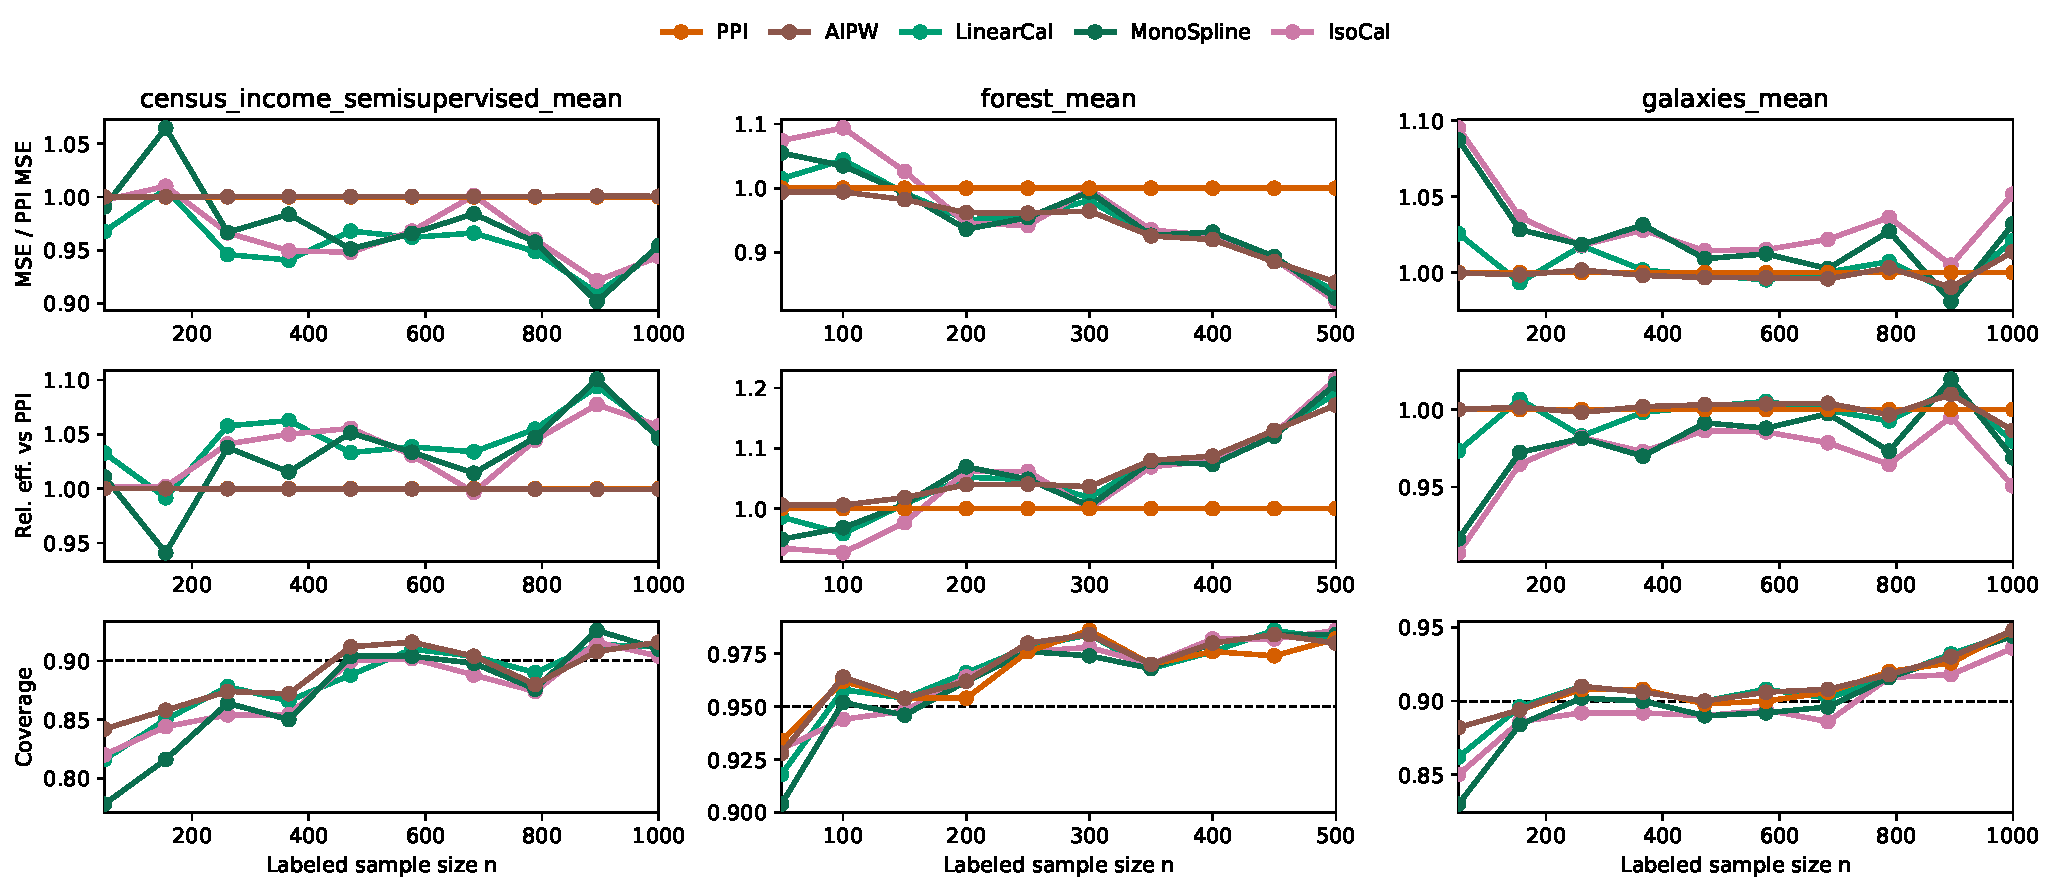
\includegraphics[width=\textwidth]{assets/fig_paper_calibration_grid.pdf}
\caption{Calibration-focused appendix comparison across the reproduced PPI benchmarks, restricted to PPI, AIPW, \texttt{LinearCal}, \texttt{MonoSpline}, and \texttt{IsoCal}. The panels report normalized MSE relative to PPI, relative efficiency versus PPI, and coverage across labeled-sample-size regimes. This figure isolates the fixed-calibration comparison that is omitted from the main-text benchmark figure for readability.}
\label{fig:ppi-calibration-appendix}
\end{figure}

\begin{figure}[hbt]
\centering
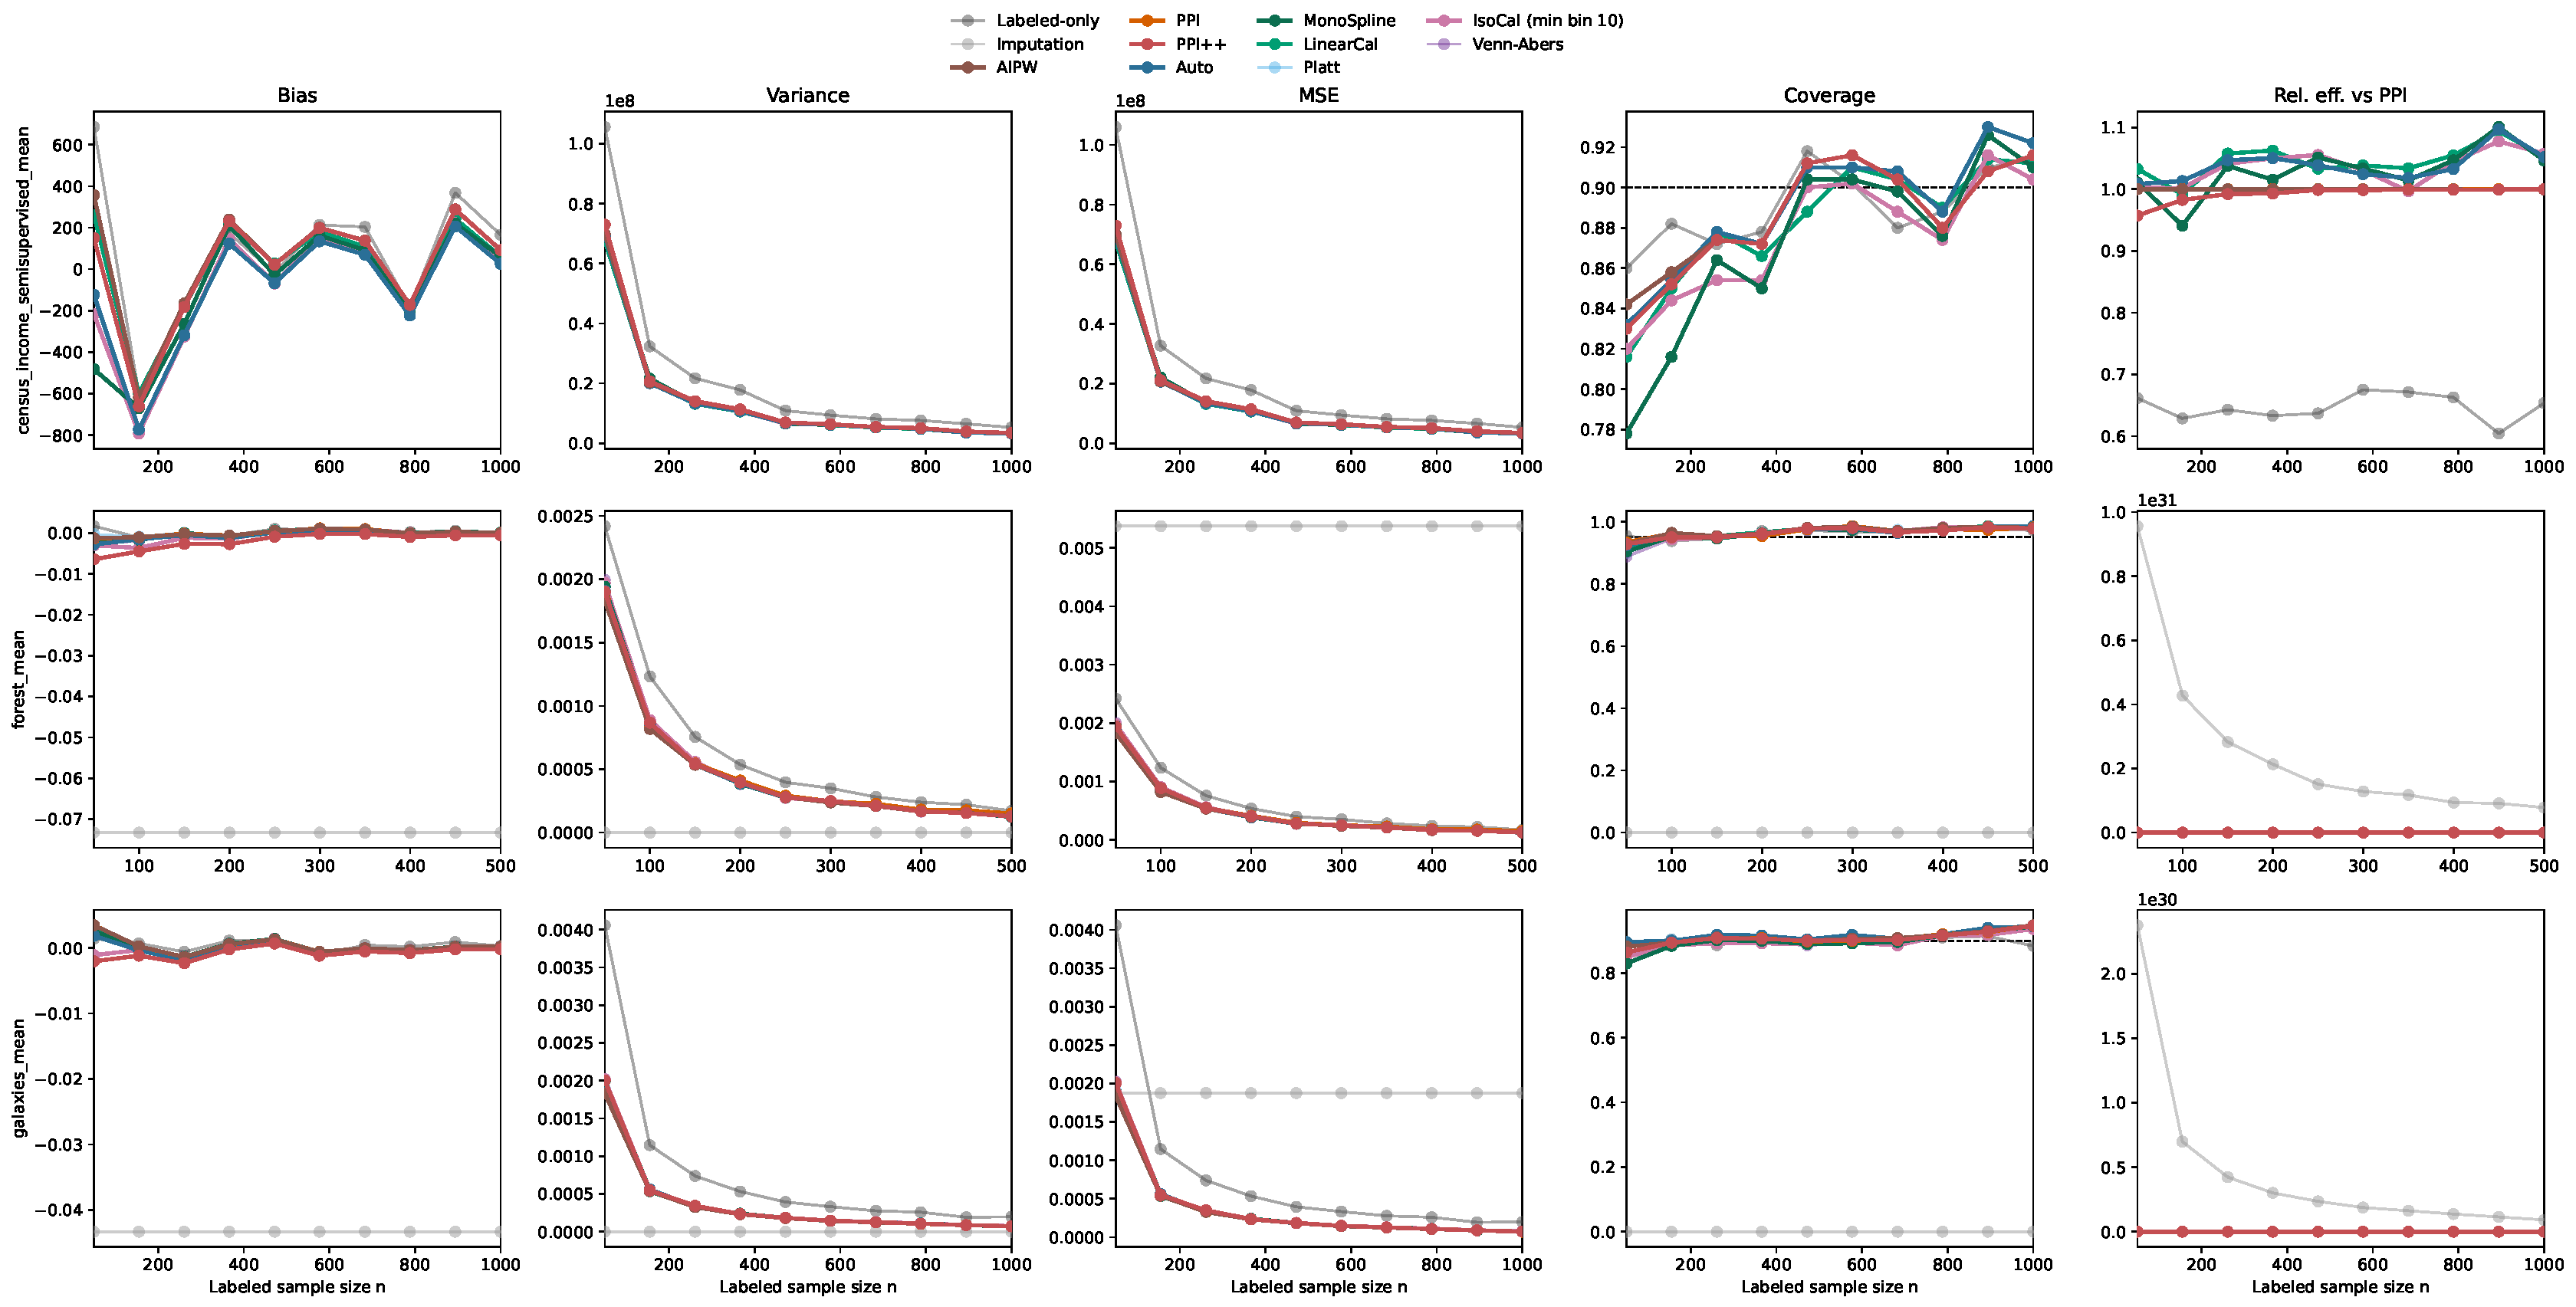
\includegraphics[width=\textwidth]{assets/fig_paper_metric_grid.pdf}
\caption{Full diagnostic grid for the reproduced PPI benchmarks, showing bias, empirical variance, normalized MSE relative to PPI, coverage, and relative efficiency versus PPI across labeled-sample-size regimes. In the normalized-MSE and relative-efficiency panels, the dashed horizontal line marks parity with PPI; in the coverage panels it marks the nominal target coverage \(1-\alpha\). \texttt{AutoCal}, \texttt{MonoSpline}, and \texttt{IsoCal} appear alongside PPI, AIPW, PPI++, \textsc{AIPW-EM}, and the fixed calibration rules, while Platt scaling and Venn--Abers appear only on the binary-outcome datasets where they are well defined.}
\label{fig:ppi-benchmarks-full}
\end{figure}

\subsection{LLM evaluator breakdown}
\label{app:llm-eval-by-evaluator}

The PPE macro-averages in the main text hide substantial evaluator heterogeneity. In particular, the largest raw-proxy failures are driven primarily by Skywork and Athene, while ArmoRM is comparatively benign and leaves all main-text estimators nearly tied. The calibration-based and efficiency-maximized methods are therefore best understood as safeguards against badly scaled reward-model margins, rather than gains that require every evaluator to be severely misaligned.

\IfFileExists{assets/table_llm_summary_appendix.tex}{
\begin{table}[hbt]
\centering
\small
\resizebox{\textwidth}{!}{\begin{tabular}{lllccc}
\toprule
Track & $n$ & Estimator & MSE / PPI & Label savings & Coverage \\
\midrule
PPE Correctness & 100 & Labeled-only & 0.346 & 0.000 & 0.927 \\
PPE Correctness & 100 & PPI & 1.000 & 0.010 & 0.904 \\
PPE Correctness & 100 & AIPW & 0.774 & 0.009 & 0.906 \\
PPE Correctness & 100 & PPI++ & 0.330 & 0.070 & 0.929 \\
PPE Correctness & 100 & AIPW-EM & 0.309 & 0.095 & 0.930 \\
PPE Correctness & 100 & LinearCal & 0.305 & 0.101 & 0.931 \\
PPE Correctness & 100 & AutoCal & 0.310 & 0.094 & 0.929 \\
PPE Correctness & 100 & MonoSpline & 0.309 & 0.092 & 0.926 \\
PPE Correctness & 100 & IsoCal & 0.309 & 0.089 & 0.925 \\
PPE Correctness & 100 & Platt & 0.304 & 0.102 & 0.930 \\
PPE Correctness & 400 & Labeled-only & 0.299 & 0.000 & 0.988 \\
PPE Correctness & 400 & PPI & 1.000 & 0.020 & 0.924 \\
PPE Correctness & 400 & AIPW & 0.405 & 0.009 & 0.941 \\
PPE Correctness & 400 & PPI++ & 0.276 & 0.083 & 0.989 \\
PPE Correctness & 400 & AIPW-EM & 0.262 & 0.103 & 0.989 \\
PPE Correctness & 400 & LinearCal & 0.260 & 0.105 & 0.989 \\
PPE Correctness & 400 & AutoCal & 0.263 & 0.102 & 0.988 \\
PPE Correctness & 400 & MonoSpline & 0.263 & 0.094 & 0.989 \\
PPE Correctness & 400 & IsoCal & 0.265 & 0.089 & 0.989 \\
PPE Correctness & 400 & Platt & 0.260 & 0.105 & 0.989 \\
PPE Human Preference & 100 & Labeled-only & 0.303 & 0.000 & 0.911 \\
PPE Human Preference & 100 & PPI & 1.000 & 0.004 & 0.897 \\
PPE Human Preference & 100 & AIPW & 0.919 & 0.004 & 0.896 \\
PPE Human Preference & 100 & PPI++ & 0.298 & 0.027 & 0.912 \\
PPE Human Preference & 100 & AIPW-EM & 0.295 & 0.031 & 0.909 \\
PPE Human Preference & 100 & LinearCal & 0.295 & 0.031 & 0.909 \\
PPE Human Preference & 100 & AutoCal & 0.297 & 0.028 & 0.908 \\
PPE Human Preference & 100 & MonoSpline & 0.297 & 0.025 & 0.903 \\
PPE Human Preference & 100 & IsoCal & 0.297 & 0.024 & 0.905 \\
PPE Human Preference & 400 & Labeled-only & 0.289 & 0.000 & 0.945 \\
PPE Human Preference & 400 & PPI & 1.000 & 0.005 & 0.915 \\
PPE Human Preference & 400 & AIPW & 0.703 & 0.004 & 0.917 \\
PPE Human Preference & 400 & PPI++ & 0.283 & 0.025 & 0.946 \\
PPE Human Preference & 400 & AIPW-EM & 0.282 & 0.028 & 0.945 \\
PPE Human Preference & 400 & LinearCal & 0.282 & 0.028 & 0.944 \\
PPE Human Preference & 400 & AutoCal & 0.282 & 0.027 & 0.944 \\
PPE Human Preference & 400 & MonoSpline & 0.282 & 0.027 & 0.942 \\
PPE Human Preference & 400 & IsoCal & 0.282 & 0.026 & 0.940 \\
\bottomrule
\end{tabular}
}
\caption{Appendix PPE-only numerical summary at \(n\in\{100,400\}\), expanding the main-text table to include the efficiency-maximized and additional fixed-calibration comparators omitted there for readability.}
\label{tab:llm-eval-summary-full}
\end{table}
}{}

\IfFileExists{assets/fig_llm_eval_by_evaluator.pdf}{
\begin{figure}[hbt]
\centering
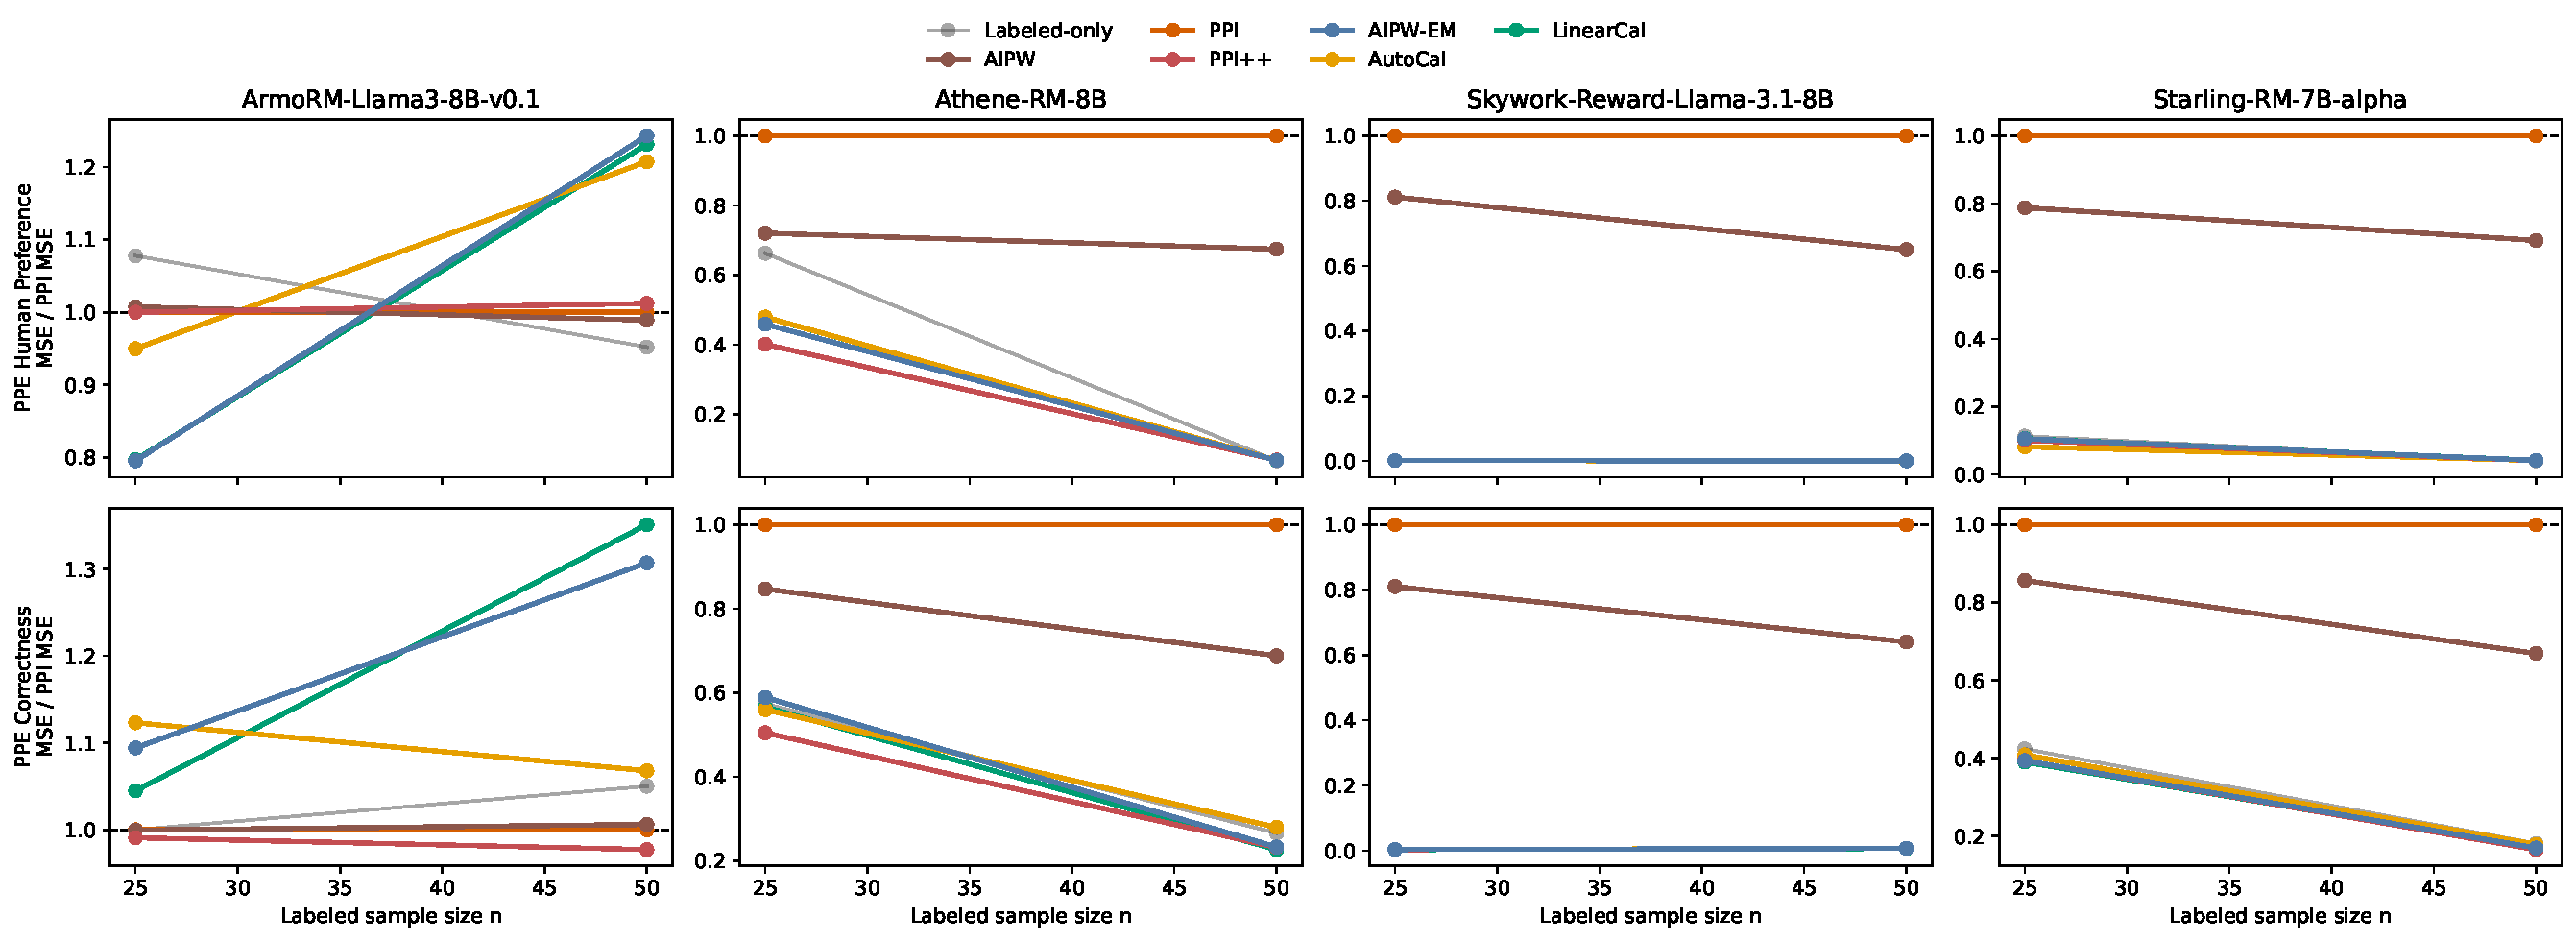
\includegraphics[width=\textwidth]{assets/fig_llm_eval_by_evaluator.pdf}
\caption{Appendix evaluator-specific PPE summary. Each panel repeats the PPE Human and PPE Correctness comparisons for one public evaluator. The large raw-proxy failures are concentrated in Skywork and Athene, while ArmoRM is much more benign.}
\label{fig:llm-eval-by-evaluator}
\end{figure}
}{}

\subsection{LLM ranking supplement}
\label{app:llm-ranking}

The PPE human-preference track also induces a downstream ranking problem across the selected target models. Using the same repeated labeled/unlabeled splits as in \cref{sec:llm-benchmark}, we summarize how well each estimator recovers the target-model ordering induced by the full-data human win shares. For each evaluator, labeled-sample size, replicate, and estimator, we rank the eight selected target models by estimated win share, compare that ordering with the ranking induced by the full-data targets, and then macro-average across evaluators. We report Spearman rank correlation, top-1 identification rate, and top-1 regret, defined as the difference in true win share between the best target model and the model selected by the estimator; see \cref{fig:llm-ppe-ranking,tab:llm-ppe-ranking}. The main pattern mirrors the mean-estimation results: calibrated and efficiency-maximized estimators substantially outperform raw PPI and raw AIPW, while remaining close to labeled-only at small \(n\). As shown in \cref{fig:llm-ppe-ranking}, \texttt{AutoCal} attains the highest average Spearman correlation at \(n=200\), about \(0.905\). By \(n=400\), \texttt{LinearCal} gives the best overall ranking quality, with Spearman correlation about \(0.941\) and top-1 identification rate about \(0.646\); selected numerical summaries are reported in \cref{tab:llm-ppe-ranking}.

\IfFileExists{assets/table_llm_ppe_ranking.tex}{
\begin{table}[hbt]
\centering
\small
\resizebox{0.74\textwidth}{!}{\begin{tabular}{llrrr}
\toprule
$n$ & Estimator & Spearman & Top-1 & Top-1 regret \\
\midrule
25 & AIPW & 0.250 & 0.625 & 0.010 \\
25 & AIPW-EM & 1.000 & 1.000 & 0.000 \\
25 & AutoCal & 1.000 & 1.000 & 0.000 \\
25 & Labeled-only & 1.000 & 1.000 & 0.000 \\
25 & LinearCal & 1.000 & 1.000 & 0.000 \\
25 & PPI & 0.250 & 0.625 & 0.010 \\
25 & PPI++ & 1.000 & 1.000 & 0.000 \\
50 & AIPW & 0.250 & 0.625 & 0.010 \\
50 & AIPW-EM & 0.500 & 0.750 & 0.006 \\
50 & AutoCal & 0.500 & 0.750 & 0.006 \\
50 & Labeled-only & 1.000 & 1.000 & 0.000 \\
50 & LinearCal & 0.500 & 0.750 & 0.006 \\
50 & PPI & 0.000 & 0.500 & 0.013 \\
50 & PPI++ & 0.750 & 0.875 & 0.003 \\
\bottomrule
\end{tabular}
}
\caption{Appendix PPE-ranking summary at selected labeled sample sizes from the LLM benchmark. Spearman and top-1 are larger-is-better, while top-1 regret is smaller-is-better.}
\label{tab:llm-ppe-ranking}
\end{table}
}{}

\IfFileExists{assets/fig_llm_ppe_ranking.pdf}{
\begin{figure}[hbt]
\centering
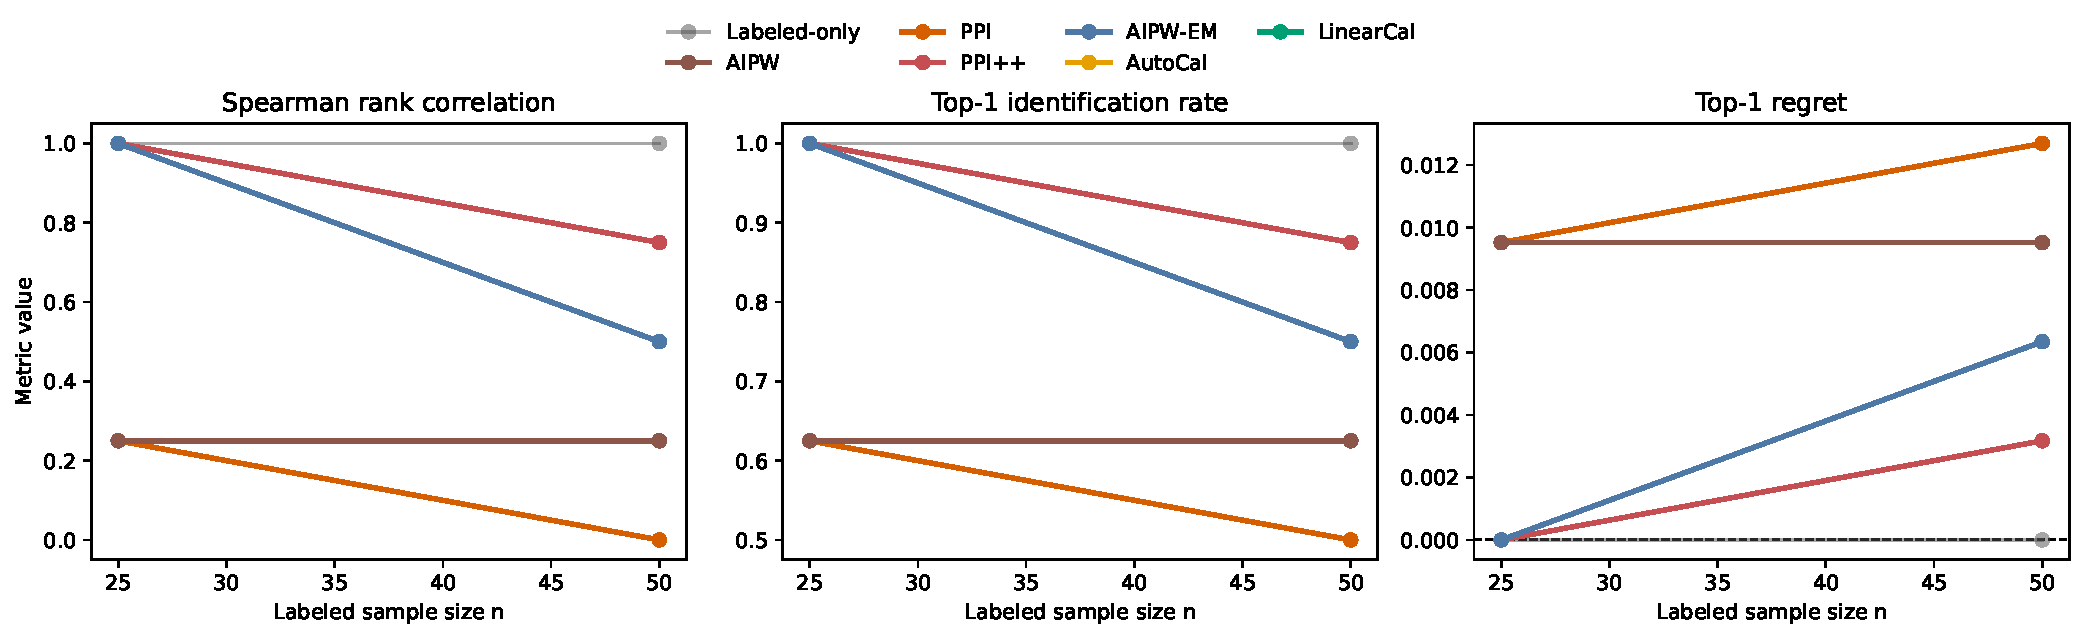
\includegraphics[width=\textwidth]{assets/fig_llm_ppe_ranking.pdf}
\caption{Appendix PPE-ranking supplement from the LLM benchmark, macro-averaged across the public evaluator models. The three panels report Spearman rank correlation, top-1 identification rate, and top-1 regret for recovering the ranking of the eight selected PPE target models from a small labeled sample plus evaluator scores.}
\label{fig:llm-ppe-ranking}
\end{figure}
}{}


\section{\texttt{Python} Code}
\label{appendix:code}

\paragraph{Code availability.}
A public repository containing the \texttt{ppi\_aipw} package, experiment scripts, and paper assets is available at
\href{https://github.com/Larsvanderlaan/ppi-aipw}{github.com/Larsvanderlaan/ppi-aipw}.
Package documentation and worked examples are hosted at
\href{https://larsvanderlaan.github.io/ppi-aipw/}{larsvanderlaan.github.io/ppi-aipw/}.

Below, we provide a minimal, self-contained implementation of the method introduced in this paper.
\subsection{Isotonic regression via XGBoost}
\begin{codeblock}
import numpy as np
import xgboost as xgb

def isoreg_with_xgboost(x, y, max_depth=15, min_child_weight=20, weights=None):
    """
    Fit a monotone calibrator f so that f(x) is nondecreasing in x.

    Parameters
    ----------
    x : array-like, shape (n,) or (n, 1)
        Predictor used for calibration. In the PPI application this is usually
        the score m(X), so x is typically one-dimensional.
    y : array-like, shape (n,)
        Labeled outcomes.
    max_depth : int, default=15
        Maximum depth for the one-round XGBoost fit.
    min_child_weight : float, default=20
        Minimum total weight in a terminal node.
    weights : array-like, optional
        Optional observation weights.

    Returns
    -------
    predict_fn : callable
        Function mapping new x values to calibrated predictions f(x).
    """
    x = np.asarray(x)
    y = np.asarray(y).reshape(-1)
    x = x.reshape(len(y), -1)

    data = xgb.DMatrix(data=x, label=y, weight=weights)
    params = {
        "max_depth": max_depth,
        "min_child_weight": min_child_weight,
        "monotone_constraints": "(" + ",".join(["1"] * x.shape[1]) + ")",
        "eta": 1.0,
        "gamma": 0.0,
        "lambda": 0.0,
        "objective": "reg:squarederror",
        "verbosity": 0,
    }
    iso_fit = xgb.train(params=params, dtrain=data, num_boost_round=1)

    def predict_fn(x_new):
        x_new = np.asarray(x_new)
        if x_new.ndim == 1:
            x_new = x_new.reshape(-1, 1)
        data_pred = xgb.DMatrix(data=x_new)
        return iso_fit.predict(data_pred)

    return predict_fn
\end{codeblock}
\subsection{Isotonic-calibrated plug-in}
\begin{codeblock}
import numpy as np
from statistics import NormalDist


def _resolve_scores(
    Y_labeled,
    X_labeled=None,
    X_unlabeled=None,
    score_fn=None,
    score_labeled=None,
    score_unlabeled=None,
):
    Y_labeled = np.asarray(Y_labeled).reshape(-1)

    if score_fn is not None:
        if X_labeled is None or X_unlabeled is None:
            raise ValueError(
                "If score_fn is provided, then X_labeled and X_unlabeled "
                "must also be provided."
            )
        score_labeled = score_fn(X_labeled)
        score_unlabeled = score_fn(X_unlabeled)
    elif score_labeled is None or score_unlabeled is None:
        raise ValueError(
            "Provide either score_fn together with X_labeled/X_unlabeled, "
            "or provide score_labeled and score_unlabeled."
        )

    score_labeled = np.asarray(score_labeled).reshape(-1)
    score_unlabeled = np.asarray(score_unlabeled).reshape(-1)

    if len(score_labeled) != len(Y_labeled):
        raise ValueError("Y_labeled and score_labeled must have the same length.")

    return Y_labeled, score_labeled, score_unlabeled


def isotonic_calibrated_plugin(
    Y_labeled,
    X_labeled=None,
    X_unlabeled=None,
    score_fn=None,
    score_labeled=None,
    score_unlabeled=None,
    alpha=0.05,
    min_obs=20,
):
    Y_labeled, score_labeled, score_unlabeled = _resolve_scores(
        Y_labeled=Y_labeled,
        X_labeled=X_labeled,
        X_unlabeled=X_unlabeled,
        score_fn=score_fn,
        score_labeled=score_labeled,
        score_unlabeled=score_unlabeled,
    )

    n = len(Y_labeled)
    N = len(score_unlabeled)
    M = n + N
    rho = n / M

    calibrator = isoreg_with_xgboost(
        x=score_labeled,
        y=Y_labeled,
        min_child_weight=min_obs,
    )

    m_labeled = calibrator(score_labeled)
    m_unlabeled = calibrator(score_unlabeled)

    psi_hat = (n * m_labeled.mean() + N * m_unlabeled.mean()) / M

    if_labeled = m_labeled - psi_hat + (Y_labeled - m_labeled) / rho
    if_unlabeled = m_unlabeled - psi_hat
    var_hat = (
        rho * np.var(if_labeled, ddof=1)
        + (1 - rho) * np.var(if_unlabeled, ddof=1)
    )
    se_hat = np.sqrt(var_hat / M)

    z = NormalDist().inv_cdf(1 - alpha / 2)
    ci = (psi_hat - z * se_hat, psi_hat + z * se_hat)

    return {
        "estimate": psi_hat,
        "standard_error": se_hat,
        "confidence_interval": ci,
    }


# Example:
# fit = isotonic_calibrated_plugin(
#     Y_labeled=Y,
#     X_labeled=X,
#     X_unlabeled=X_tilde,
#     score_fn=m,
# )
\end{codeblock}

\subsection{Linear calibration}
\begin{codeblock}
import numpy as np
from statistics import NormalDist


def _resolve_scores(
    Y_labeled,
    X_labeled=None,
    X_unlabeled=None,
    score_fn=None,
    score_labeled=None,
    score_unlabeled=None,
):
    Y_labeled = np.asarray(Y_labeled).reshape(-1)

    if score_fn is not None:
        if X_labeled is None or X_unlabeled is None:
            raise ValueError(
                "If score_fn is provided, then X_labeled and X_unlabeled "
                "must also be provided."
            )
        score_labeled = score_fn(X_labeled)
        score_unlabeled = score_fn(X_unlabeled)
    elif score_labeled is None or score_unlabeled is None:
        raise ValueError(
            "Provide either score_fn together with X_labeled/X_unlabeled, "
            "or provide score_labeled and score_unlabeled."
        )

    score_labeled = np.asarray(score_labeled).reshape(-1)
    score_unlabeled = np.asarray(score_unlabeled).reshape(-1)

    if len(score_labeled) != len(Y_labeled):
        raise ValueError("Y_labeled and score_labeled must have the same length.")

    return Y_labeled, score_labeled, score_unlabeled


def linear_calibrated_plugin(
    Y_labeled,
    X_labeled=None,
    X_unlabeled=None,
    score_fn=None,
    score_labeled=None,
    score_unlabeled=None,
    alpha=0.05,
):
    Y_labeled, score_labeled, score_unlabeled = _resolve_scores(
        Y_labeled=Y_labeled,
        X_labeled=X_labeled,
        X_unlabeled=X_unlabeled,
        score_fn=score_fn,
        score_labeled=score_labeled,
        score_unlabeled=score_unlabeled,
    )

    n = len(Y_labeled)
    N = len(score_unlabeled)
    M = n + N
    rho = n / M

    X_design = np.column_stack([np.ones(n), score_labeled])
    beta_hat, _, _, _ = np.linalg.lstsq(X_design, Y_labeled, rcond=None)

    def calibrator(score):
        score = np.asarray(score).reshape(-1)
        return beta_hat[0] + beta_hat[1] * score

    m_labeled = calibrator(score_labeled)
    m_unlabeled = calibrator(score_unlabeled)

    psi_hat = (n * m_labeled.mean() + N * m_unlabeled.mean()) / M

    if_labeled = m_labeled - psi_hat + (Y_labeled - m_labeled) / rho
    if_unlabeled = m_unlabeled - psi_hat
    var_hat = (
        rho * np.var(if_labeled, ddof=1)
        + (1 - rho) * np.var(if_unlabeled, ddof=1)
    )
    se_hat = np.sqrt(var_hat / M)

    z = NormalDist().inv_cdf(1 - alpha / 2)
    ci = (psi_hat - z * se_hat, psi_hat + z * se_hat)

    return {
        "estimate": psi_hat,
        "standard_error": se_hat,
        "confidence_interval": ci,
    }


# Example:
# fit = linear_calibrated_plugin(
#     Y_labeled=Y,
#     score_labeled=mX,
#     score_unlabeled=mX_tilde,
# )
\end{codeblock}


\end{document}
